\chapter{Repository Information and Notes for Reproduction}
\label{appendix:repository}

All source code for this project is available on GitHub at \url{https://github.com/1592800-ox/ox-dissertation.git}. 

\section{Repository Structure}

For easier identification, the training models stored in `trained-models' directory follows a uniform naming convention: `model-\{data-source\}-\{cell-line\}-\{PE\}-\{fold\}.pth/pkl/json'. 

\section{Notes for Reproduction}

All data in format other than the original CSV files or the standardized format were deleted before submission to meet the file size limit. Therefore, the data preprocessing steps should be run before training the models. The conversion scripts are available in the `models/data/std' folder, and must be run when the working directory is set to the same directory as the script.

The web application used the bagging model to process the input data, as it was the best performing model in the study. However, the PRIDICT model has a substantially longer inference time compared to the sum of all the other models. Therefore, the bagging module was modified to not use the PRIDICT model in the current state of the repository. As a result, before trying to run the bagging model and reproduce the results, the commented out lines corresponding to the PRIDICT model in the \verb|base_learners| dictionary should first be uncommented.


\chapter{Full List of Features Investigated}
\label{appendix:features}

For individual feature such as tm-pbs, $\checkmark$ indicates that the feature was used in the final model and $\times$ indicates that the feature was not used in the final model. At the same time, for a group of features, if at least one feature was used in the final model, a $\circ$ is placed in the last column. 

% table of features and their explanations
\begin{longtable}{|p{0.3\textwidth}|p{0.5\textwidth}|p{0.1\textwidth}|}
    \hline
    \textbf{Feature} & \textbf{Explanation} & \textbf{Top 24} \\ 
    \hline
    \endfirsthead

    \hline
    \textbf{Feature} & \textbf{Explanation} & \textbf{Top 24} \\ 
    \hline
    \endhead

    \hline
    \endfoot

    \hline
    \endlastfoot

    tm-rha & Melting temperature of RHA RNA sequences & $\checkmark$ \\
    \hline
    tm-pbs & Melting temperature of PBS RNA sequences & $\checkmark$ \\
    \hline
    tm-spacer & Melting temperature of spacer RNA sequences & $\times$ \\
    \hline
    tm-extension & Melting temperature of extension RNA sequences & $\times$ \\
    \hline
    max-cas & Maximum number of consecutive A bases in the cDNA of extension as well as protospacer sequence & $\times$ \\
    \hline
    max-cts & Maximum number of consecutive T bases in the cDNA of extension as well as protospacer sequence & $\checkmark$ \\
    \hline
    max-cgs & Maximum number of consecutive G bases in the cDNA of extension as well as protospacer sequence & $\times$ \\
    \hline
    max-ccs & Maximum number of consecutive C bases in the cDNA of extension as well as protospacer sequence & $\times$ \\
    \hline
    mfe-pbs & Minimum free energy of PBS RNA sequences & $\times$ \\
    \hline
    mfe-rt & Minimum free energy of RT primer RNA sequences & $\times$ \\
    \hline
    mfe-spacer & Minimum free energy of spacer RNA sequences & $\times$ \\
    \hline
    mfe-extension & Minimum free energy of extension RNA sequences & $\checkmark$ \\
    \hline
    a-at-protospacer-position-x & Number of A bases at position x in the protospacer sequence & $\circ$ \\
    \hline
    t-at-protospacer-position-x & Number of T bases at position x in the protospacer sequence & $\circ$ \\
    \hline
    g-at-protospacer-position-x & Number of G bases at position x in the protospacer sequence & $\circ$ \\
    \hline
    c-at-protospacer-position-x & Number of C bases at position x in the protospacer sequence & $\circ$ \\
    \hline
    edit-type-replace & Whether the edit type is replace & $\checkmark$ \\
    \hline
    edit-type-insert & Whether the edit type is insert & $\times$ \\
    \hline
    edit-type-delete & Whether the edit type is delete & $\times$ \\
    \hline
    rha-length & Length of the RHA RNA sequence & $\checkmark$ \\
    \hline
    pbs-length & Length of the PBS RNA sequence & $\checkmark$ \\
    \hline
    lha-length & Length of the LHA RNA sequence & $\checkmark$ \\
    \hline
    pam-disrupted & Whether the PAM sequence is disrupted & $\checkmark$ \\
    \hline
    spcas9-score & The prediction score of DeepSpCas9 model on the spacer sequence & $\checkmark$ \\
    \hline
    \caption{List of Features Investigated in the Study}
    \label{table:features}
\end{longtable}


\chapter{Additional Figures}
\label{appendix:additional-figures}

\section{Additional Figures for Error Analysis}
\label{appendix:error-analysis-figures}





The same error analysis conducted on \autoref{fig:error-analysis} was also conducted on the PRIDICT datasets. The result is very similar, but with major difference in terms of the correlation between PRIDICT and DeepPrime. The correlation between the two deep learning is much weaker, with the Spearman correlation around 0.7. The more dataset specific differences are pointed out in the caption of \autoref{fig:error-analysis-adv-pe2}, \autoref{fig:error-analysis-hek293t-pe2}, \autoref{fig:error-analysis-k562-pe2}, and \autoref{fig:error-analysis-k562mlh1dn-pe2}.

Due to the smaller data size, the downsampling and smoothing were done with a lower ratio of 10:1 and a smaller moving window of size 100, respectively. 

\newpage

\begin{figure}[!htb]
    \centering
    \subfigure[][Error Distribution]{
        \centering
        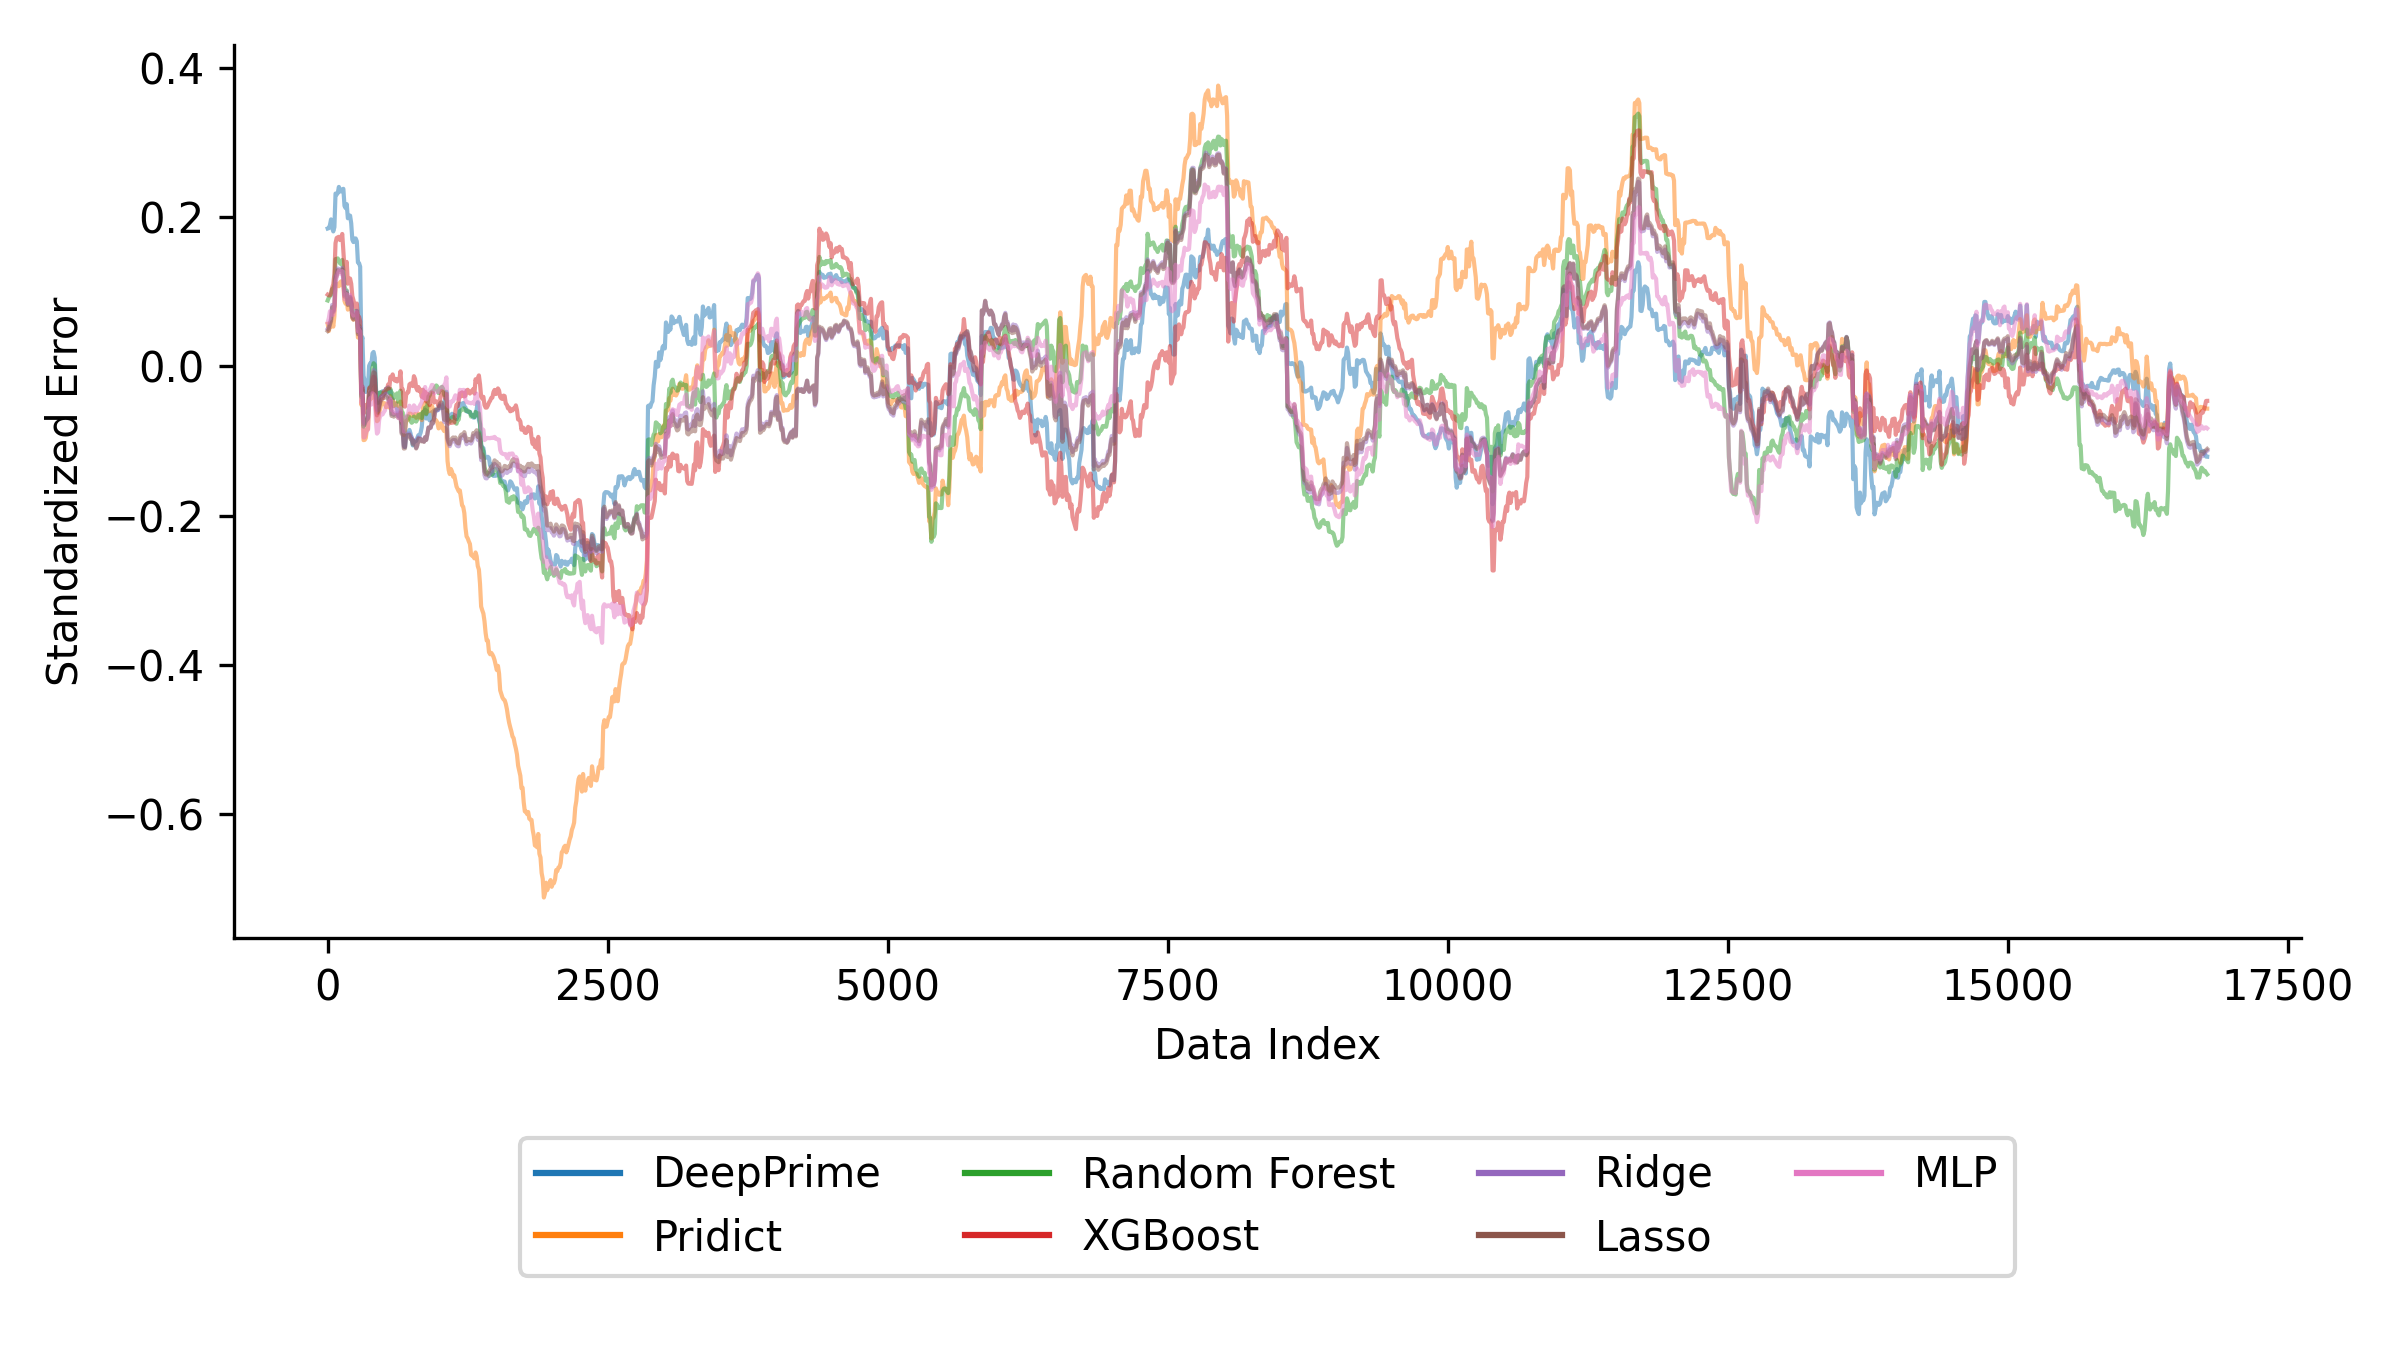
\includegraphics[width=\textwidth]{error_comparison_pd-adv-pe2.png}
        % \caption{Error Distribution of the Individual Models}
        \label{fig:error-distribution-adv-pe2}
    }
    \subfigure[][Pearson Correlation]{
        \centering
        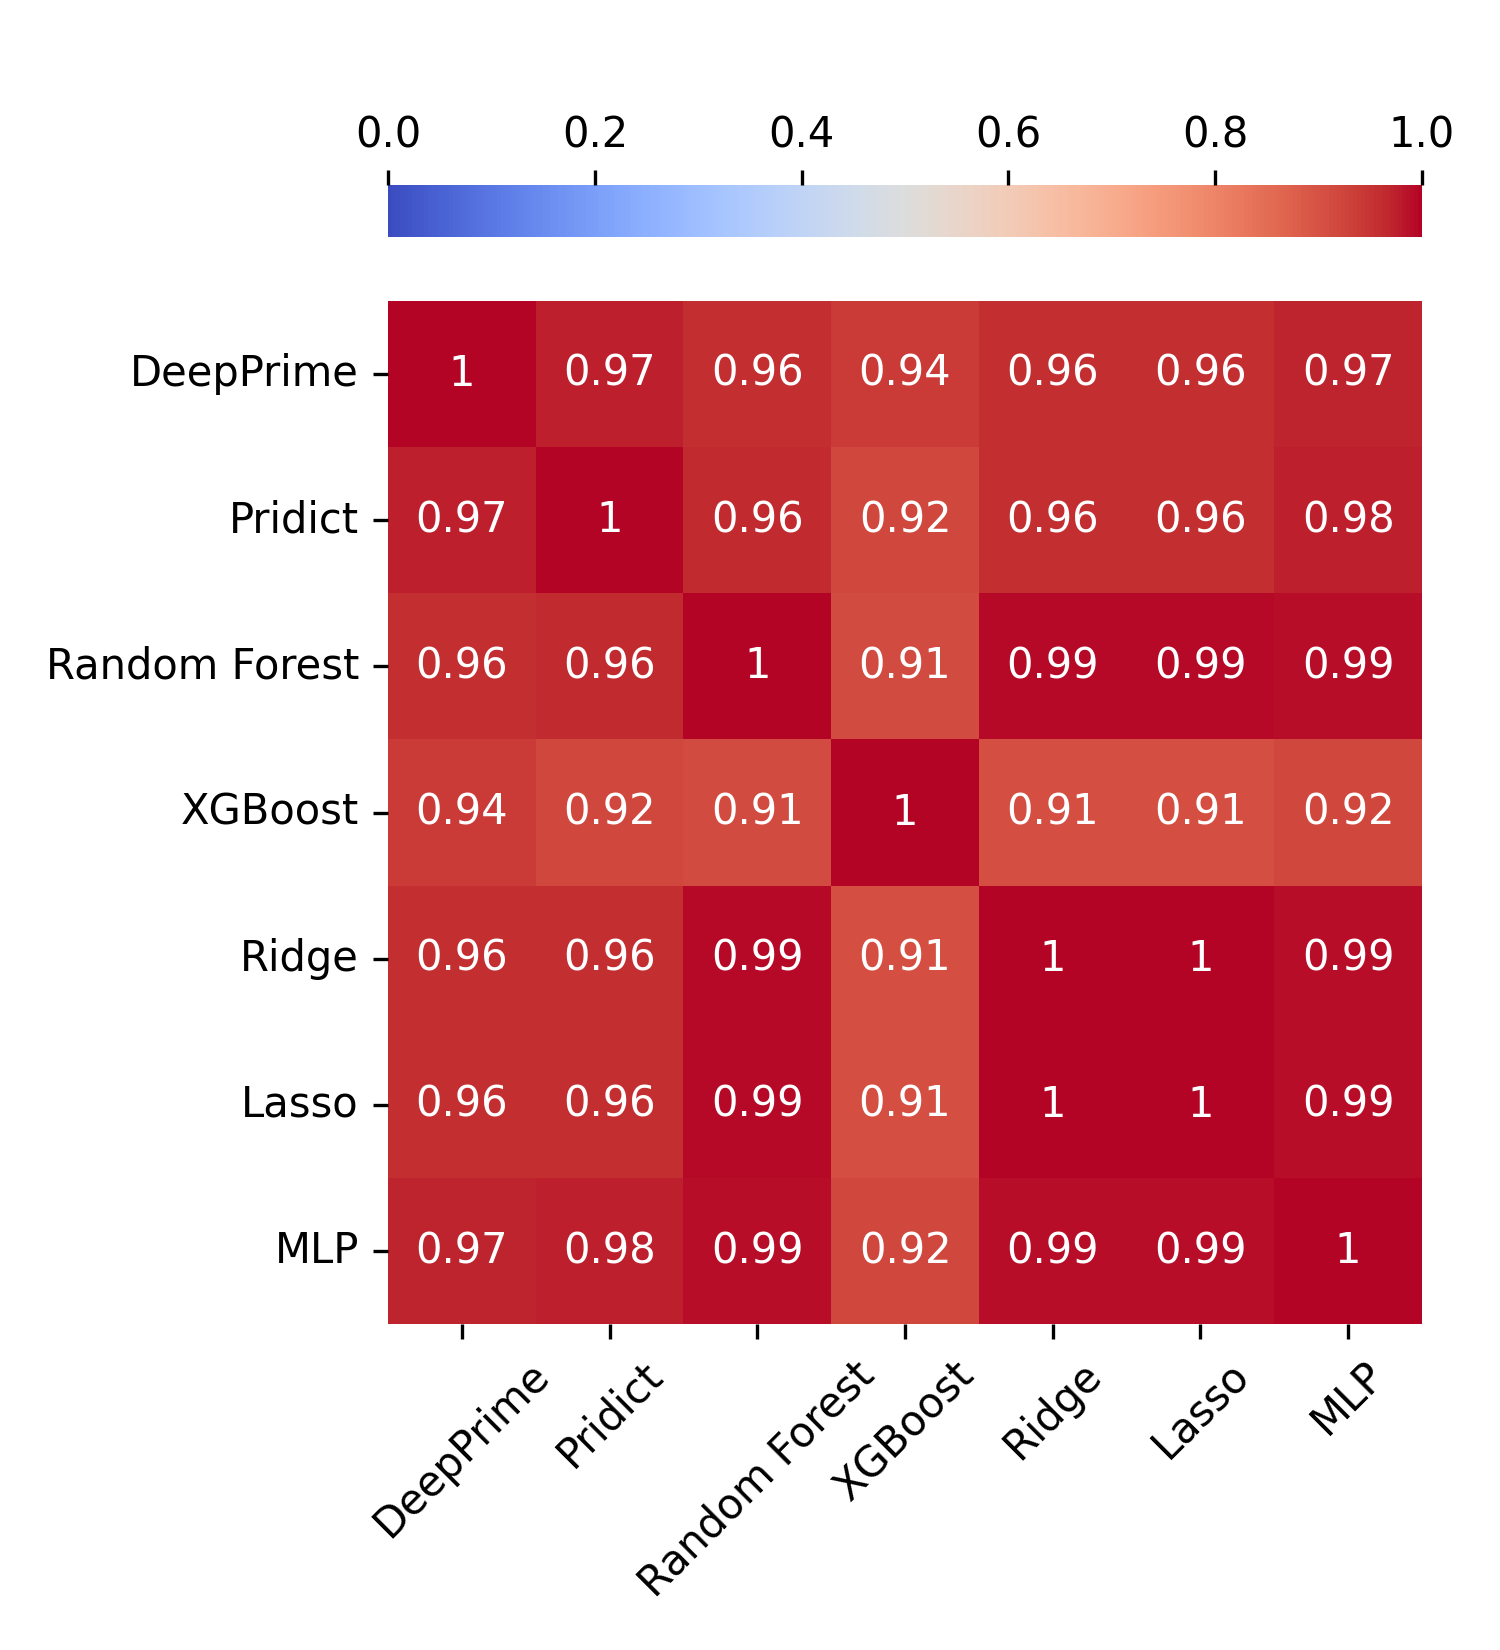
\includegraphics[width=0.49\textwidth]{error_correlation_pd-adv-pe2_pearson.png}
        % \caption{Pearson Correlation of the Error of the Individual Models}
        \label{fig:pearson-correlation-adv-pe2}
    }%
    \subfigure[][Spearman Correlation]{
        \centering
        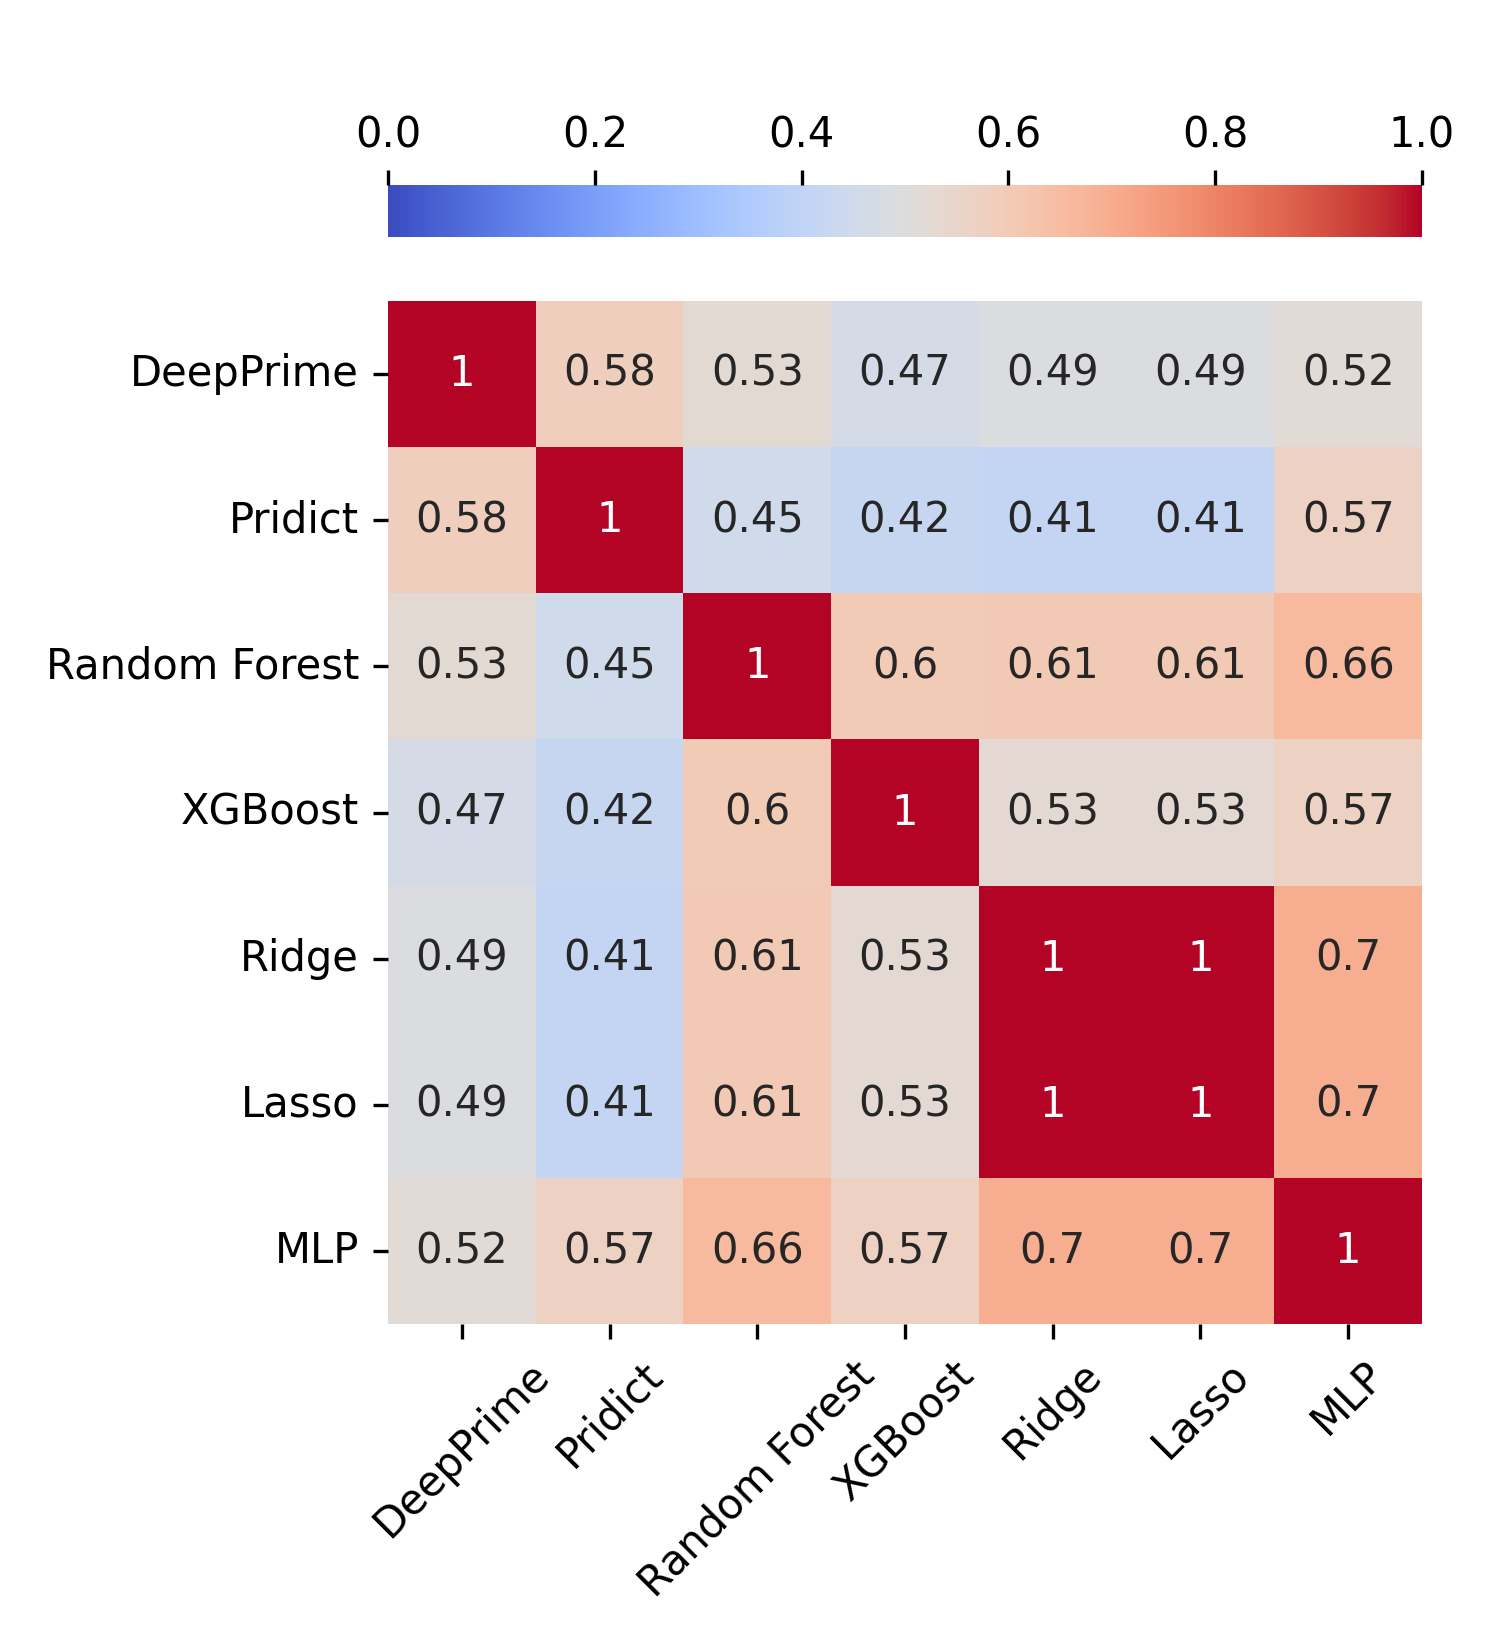
\includegraphics[width=0.49\textwidth]{error_correlation_pd-adv-pe2_spearman.png}
        % \caption{Spearman Correlation of the Error of the Individual Models}
        \label{fig:spearman-correlation-adv-pe2}
    }
    \caption[Error Analysis of the Individual Models on PRIDICT Adv PE2 dataset]{Error Analysis of the Individual Models on the PRIDICT Adv PE2 dataset. \textbf{(a)} The distribution of the error of the individual models at each example, smoothened using a moving window of size 100, and downsampled with a ratio of 10:1 for better visibility; \textbf{(b)} The Pearson correlation of the error of the individual models. \textbf{(c)} The Spearman correlation of the error of the individual models.}
    \label{fig:error-analysis-adv-pe2}
\end{figure}
\newpage

\begin{figure}[!htb]
    \centering
    \subfigure[][Error Distribution]{
        \centering
        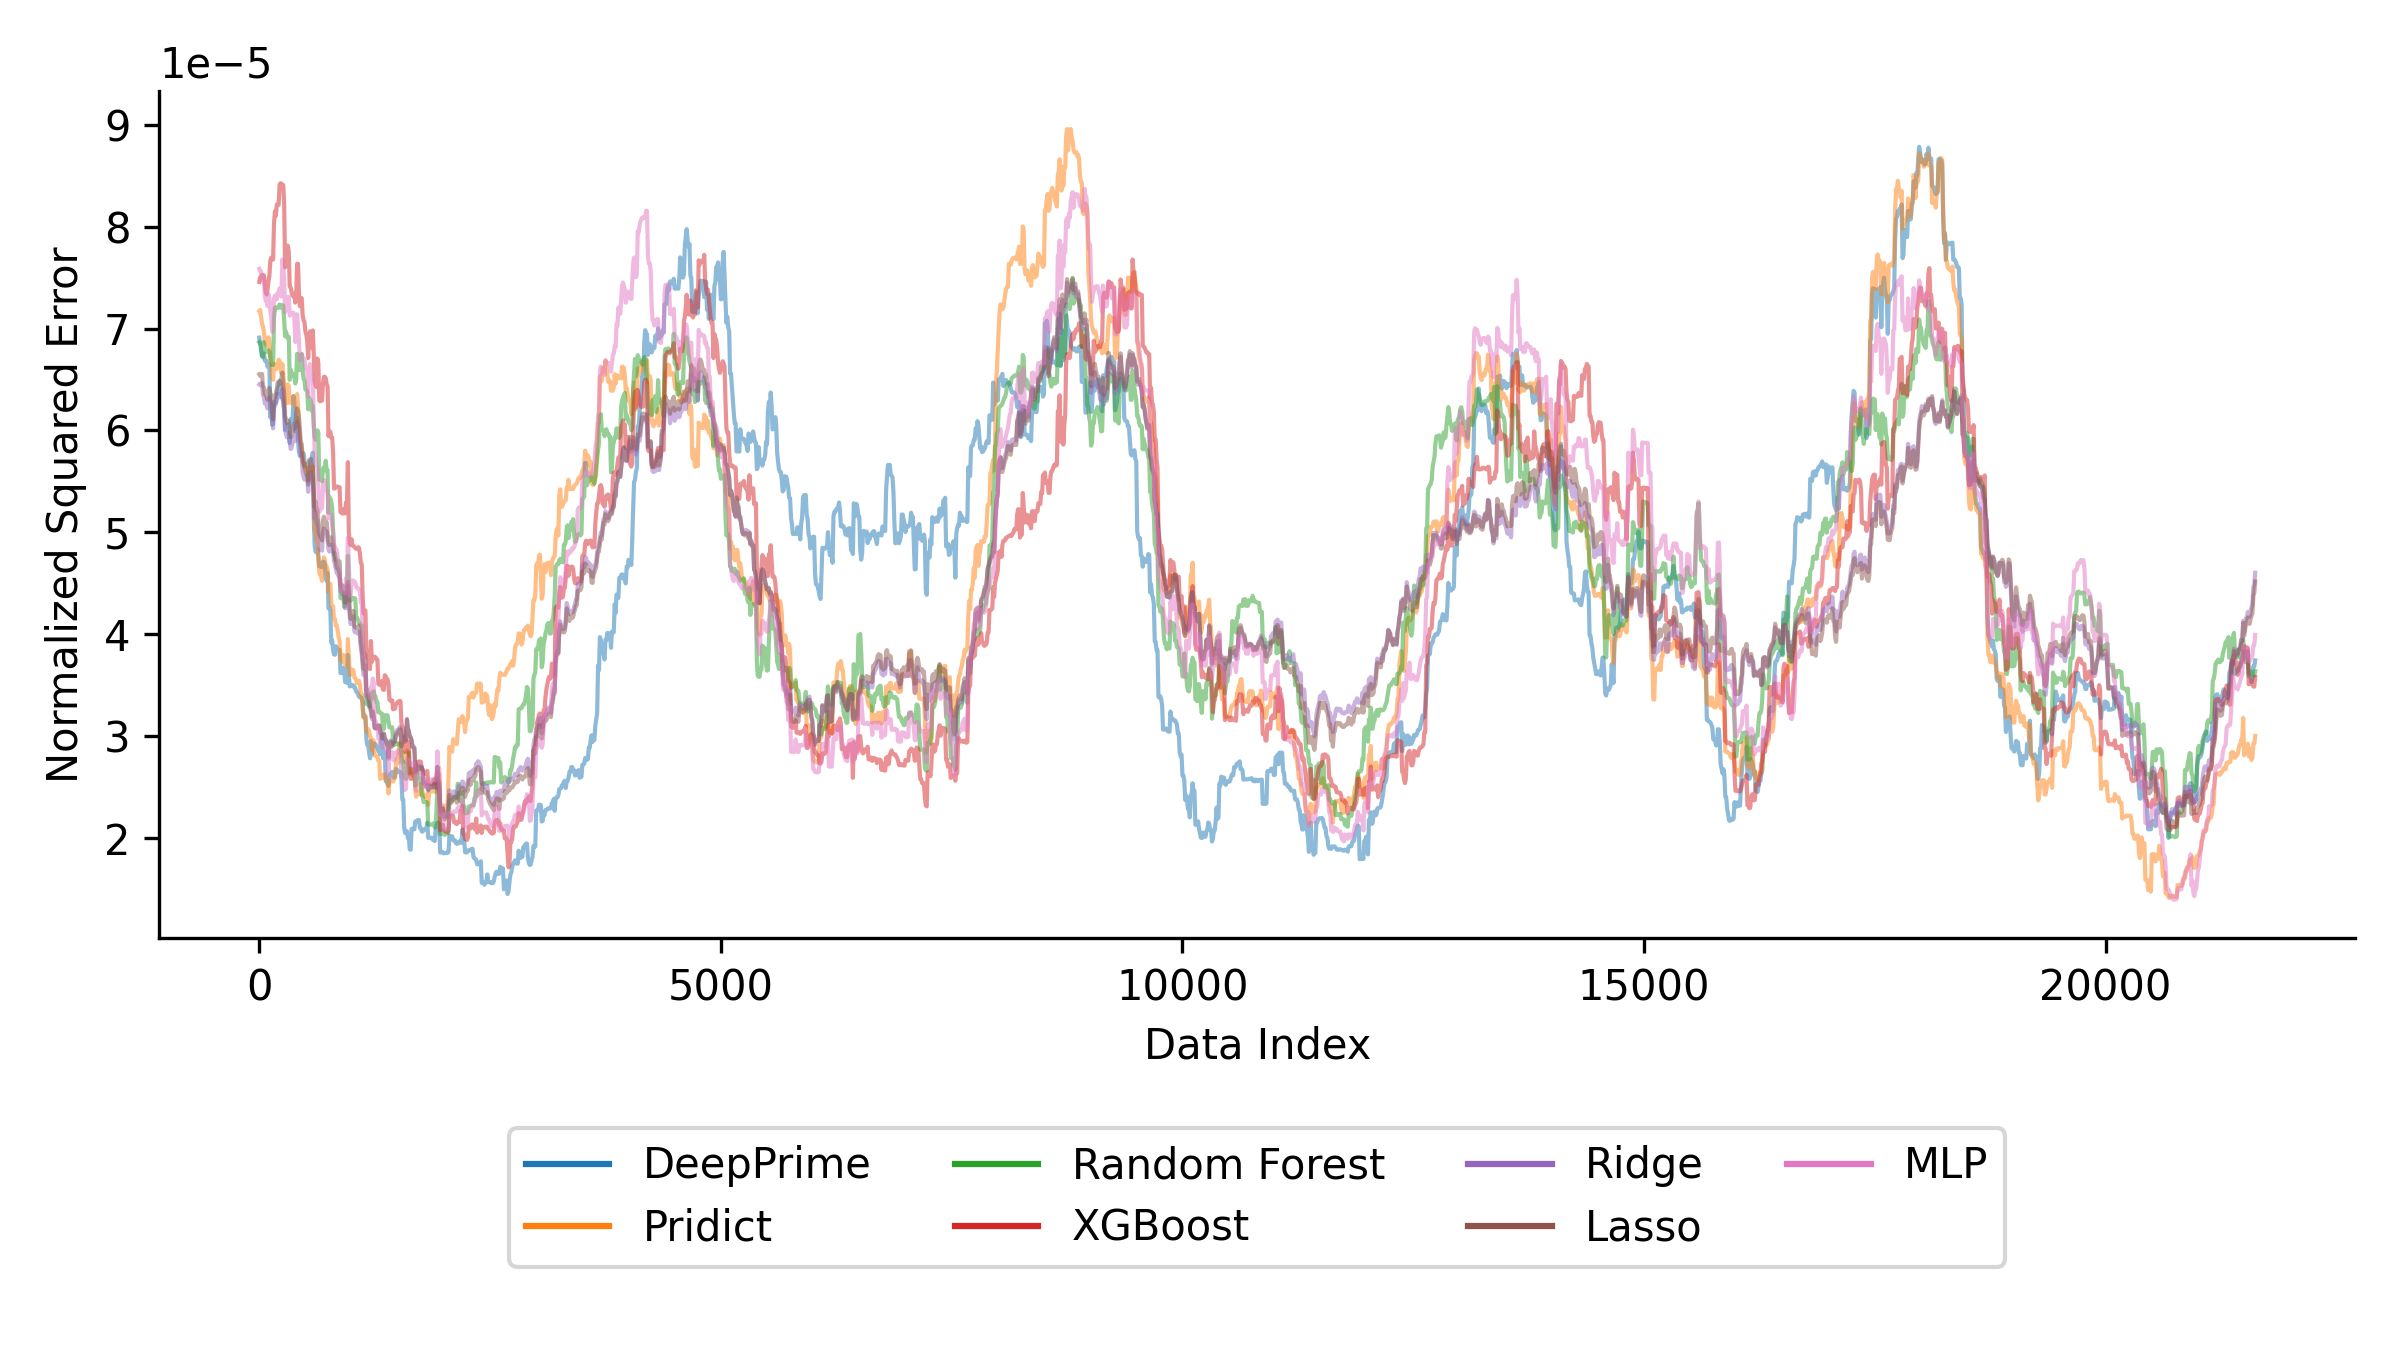
\includegraphics[width=\textwidth]{error_comparison_pd-hek293t-pe2.png}
        % \caption{Error Distribution of the Individual Models}
        \label{fig:error-distribution-hek293t-pe2}
    }
    \subfigure[][Pearson Correlation]{
        \centering
        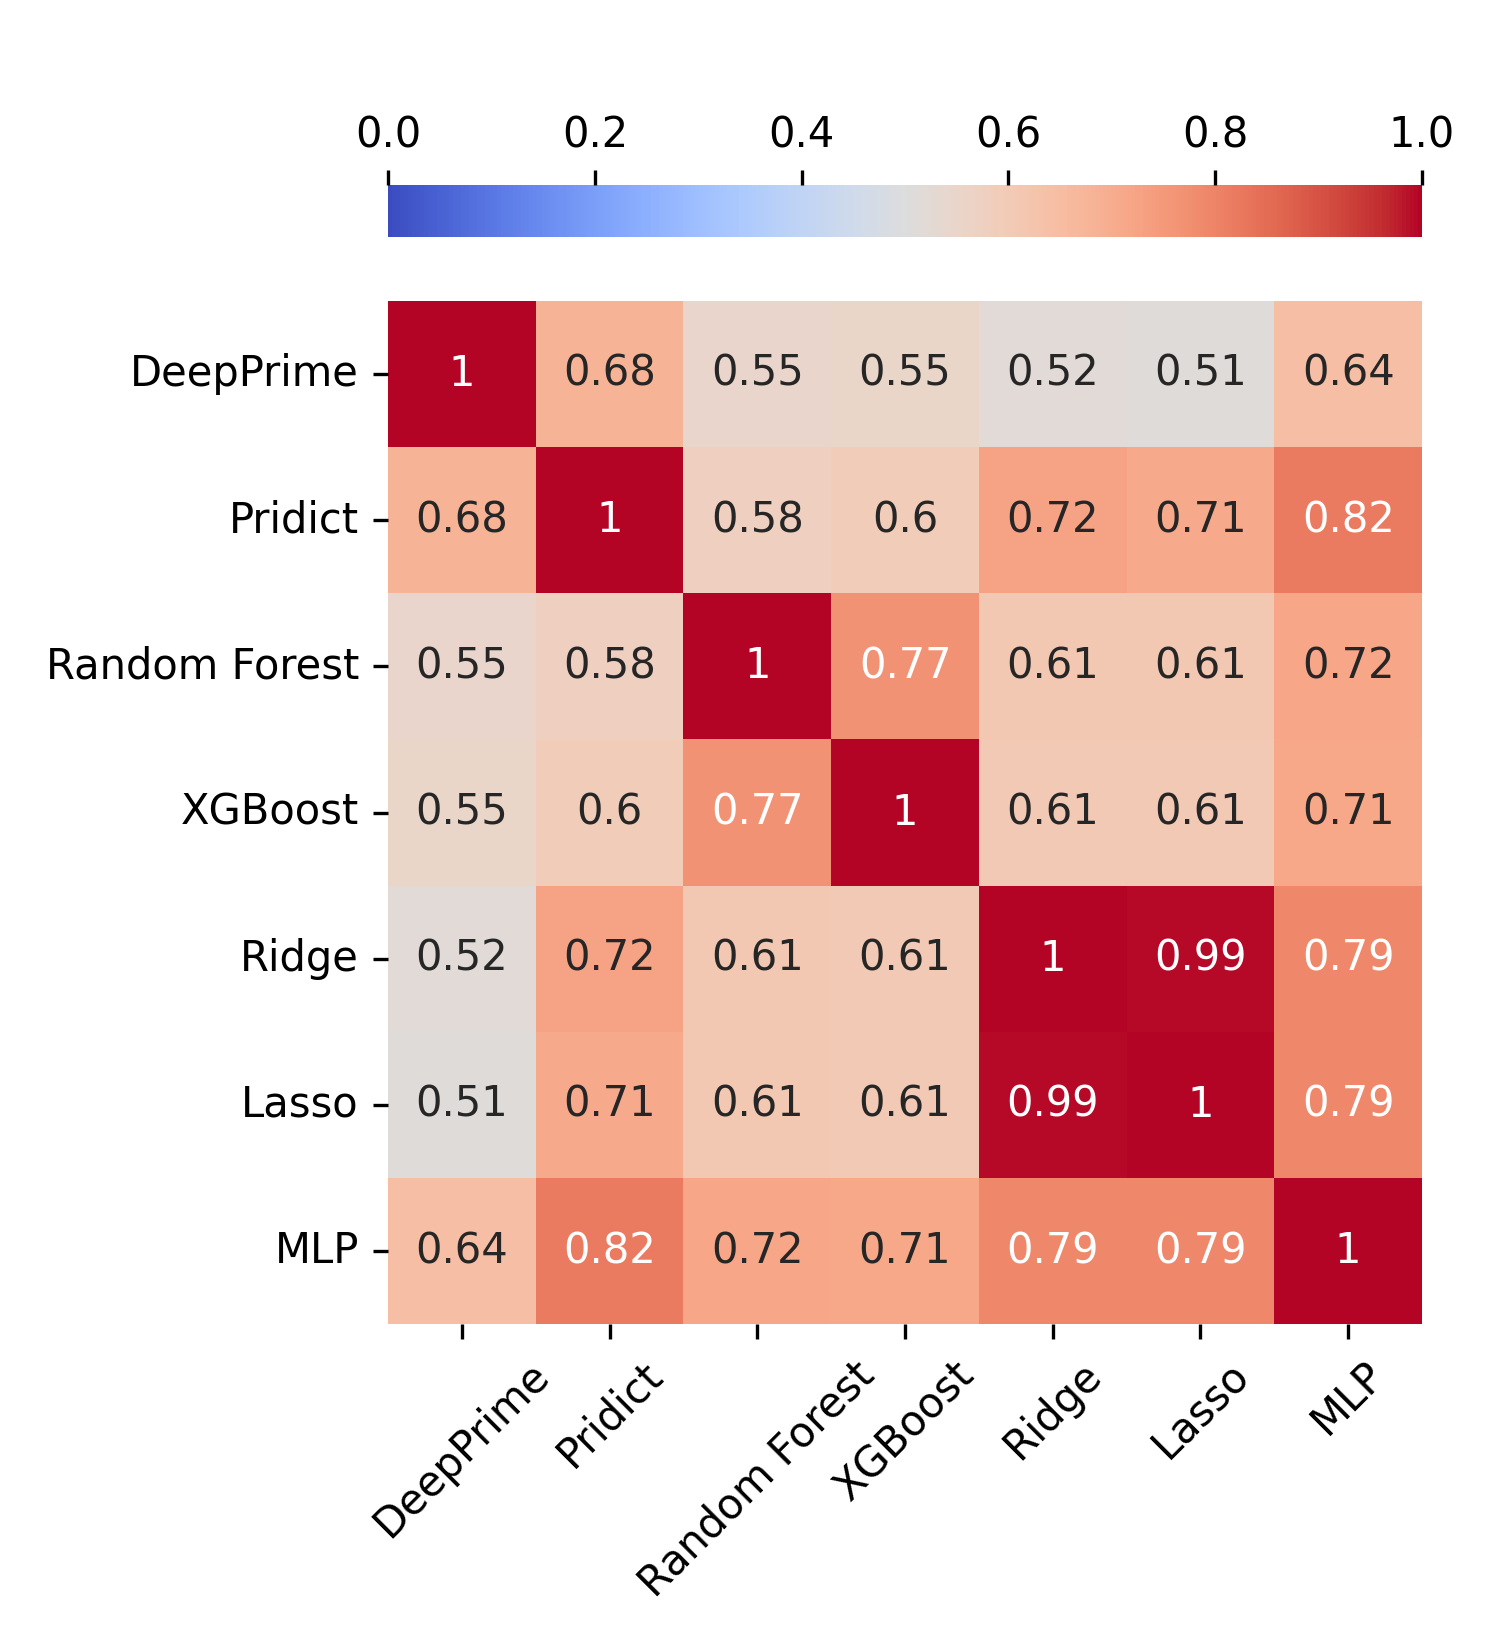
\includegraphics[width=0.49\textwidth]{error_correlation_pd-hek293t-pe2_pearson.png}
        % \caption{Pearson Correlation of the Error of the Individual Models}
        \label{fig:pearson-correlation-hek293t-pe2}
    }%
    \subfigure[][Spearman Correlation
    ]{
        \centering
        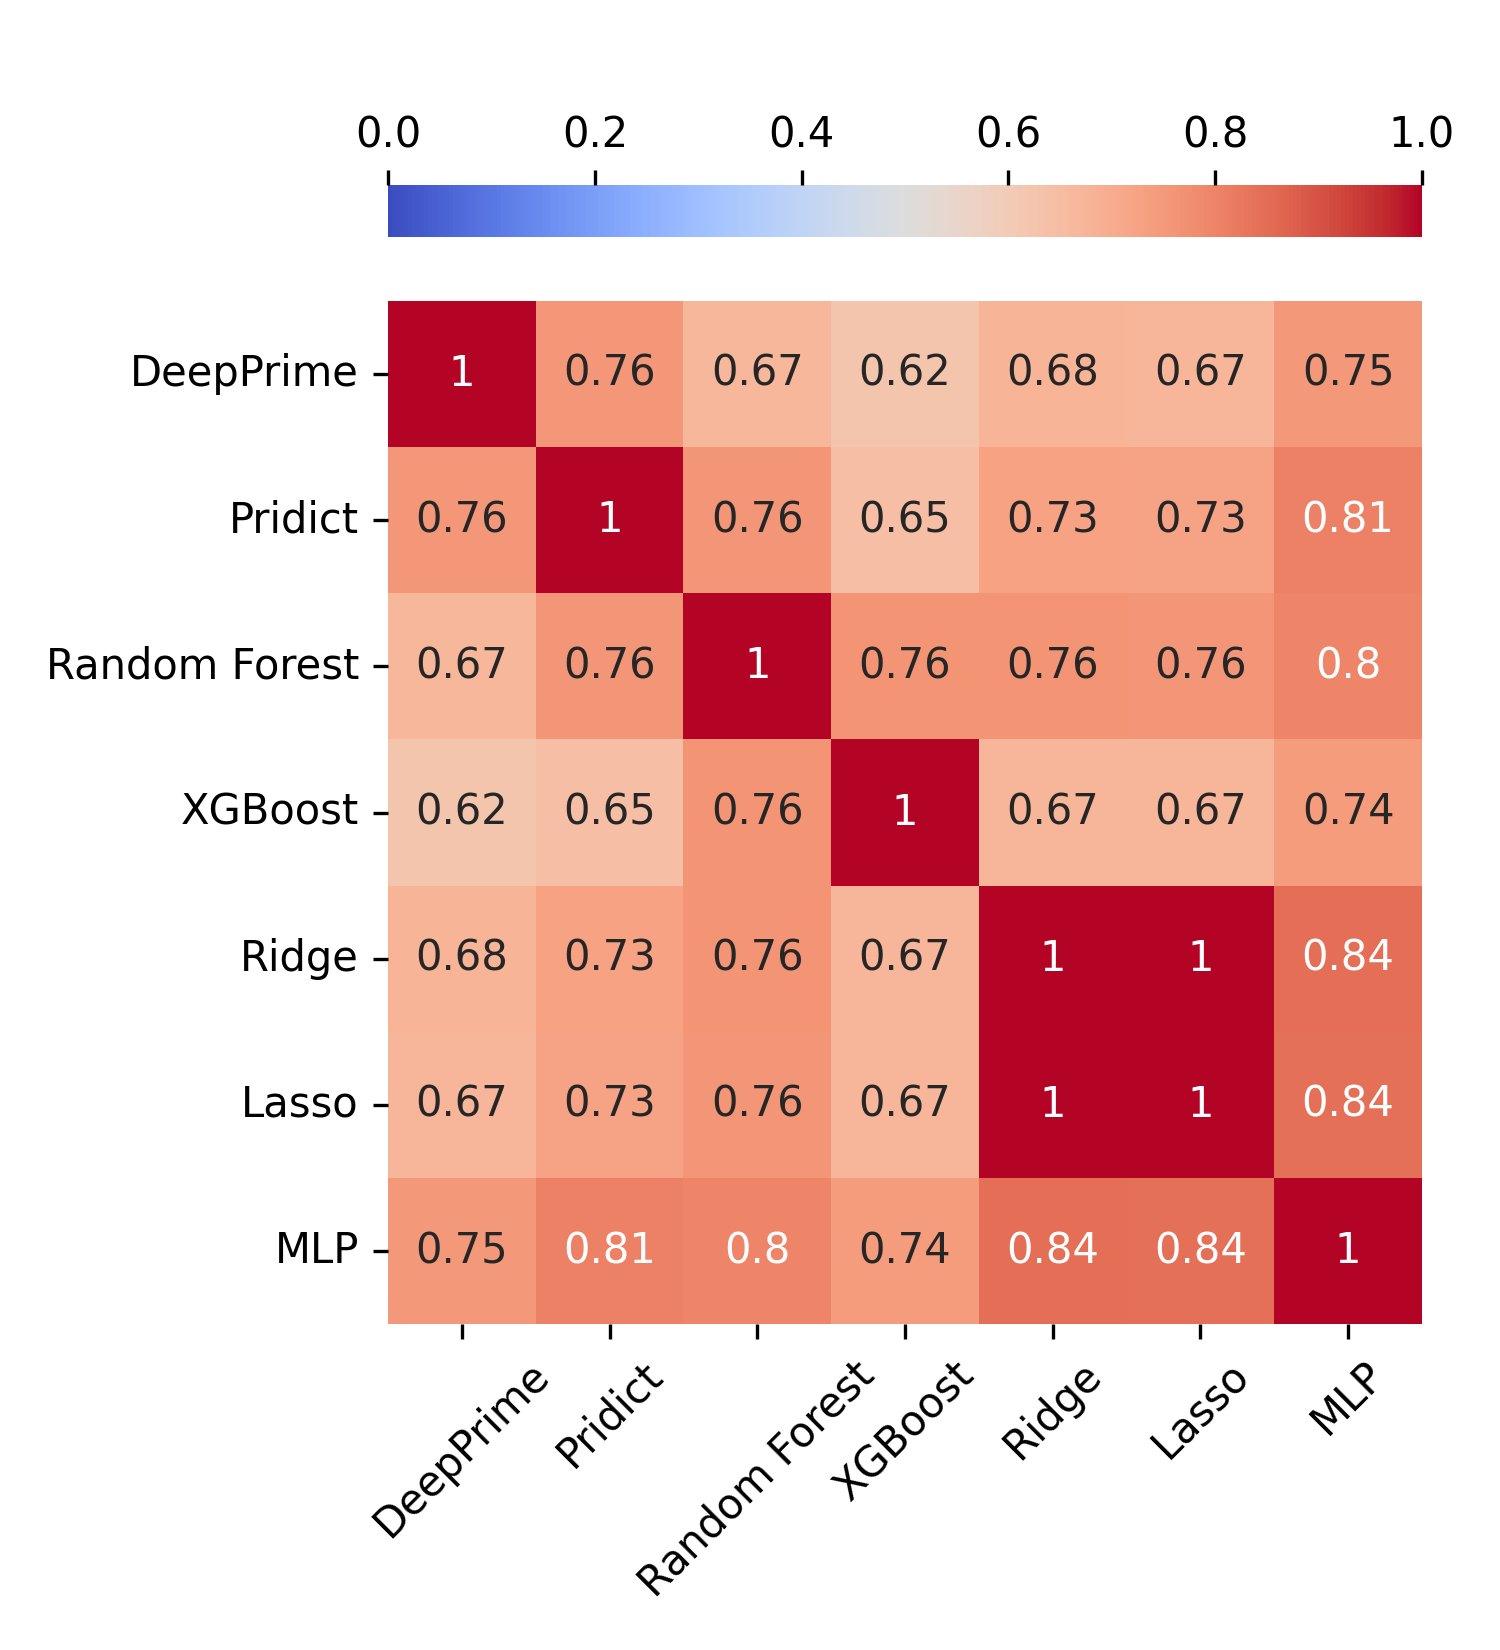
\includegraphics[width=0.49\textwidth]{error_correlation_pd-hek293t-pe2_spearman.png}
        % \caption{Spearman Correlation of the Error of the Individual Models}
        \label{fig:spearman-correlation-hek293t-pe2}
    }
    \caption[Error Analysis of the Individual Models on PRIDICT HEK293T PE2 dataset]{Error Analysis of the Individual Models on the PRIDICT HEK293T PE2 dataset. \textbf{(a)}, \textbf{(b)}, and \textbf{(c)} are the same as \autoref{fig:error-analysis-adv-pe2}. Pearson's r is much weaker, possibly due to a more balanced target value distribution as we have seen in \autoref{fig:imbalanced} The MLP is strongly correlated with all other models, especially PRIDICT.}
    \label{fig:error-analysis-hek293t-pe2}
\end{figure}
\newpage

\begin{figure}[!htb]
    \centering
    \subfigure[][Error Distribution]{
        \centering
        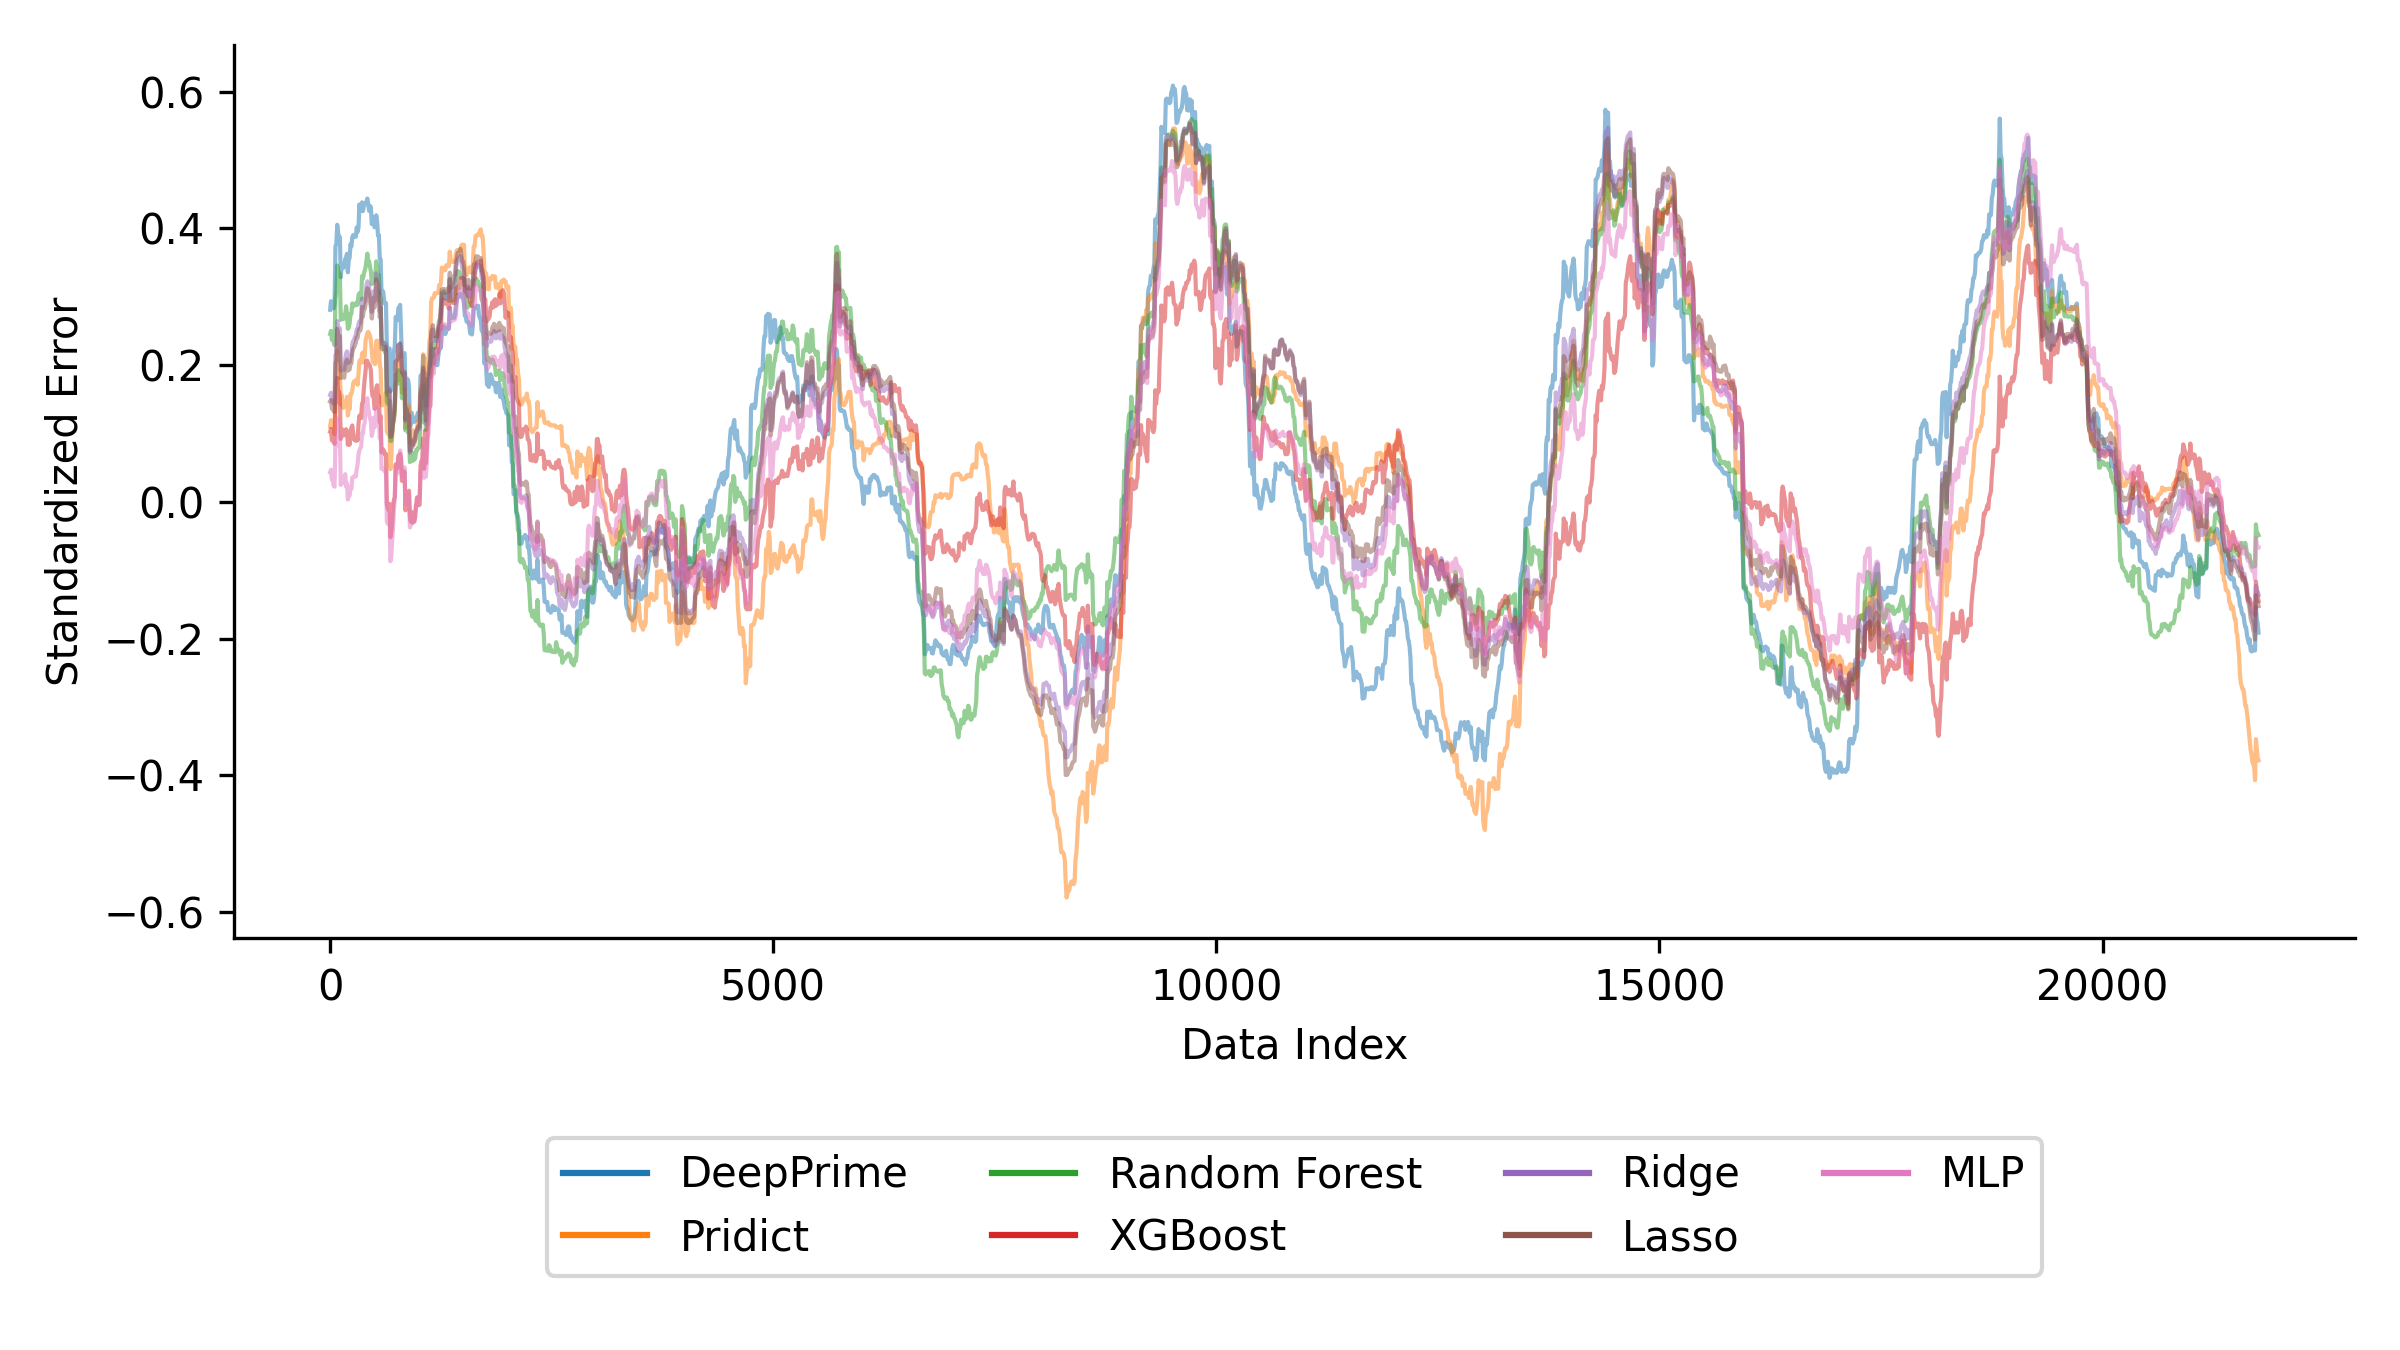
\includegraphics[width=\textwidth]{error_comparison_pd-k562-pe2.png}
        % \caption{Error Distribution of the Individual Models}
        \label{fig:error-distribution-k562-pe2}
    }
    \subfigure[][Pearson Correlation]{
        \centering
        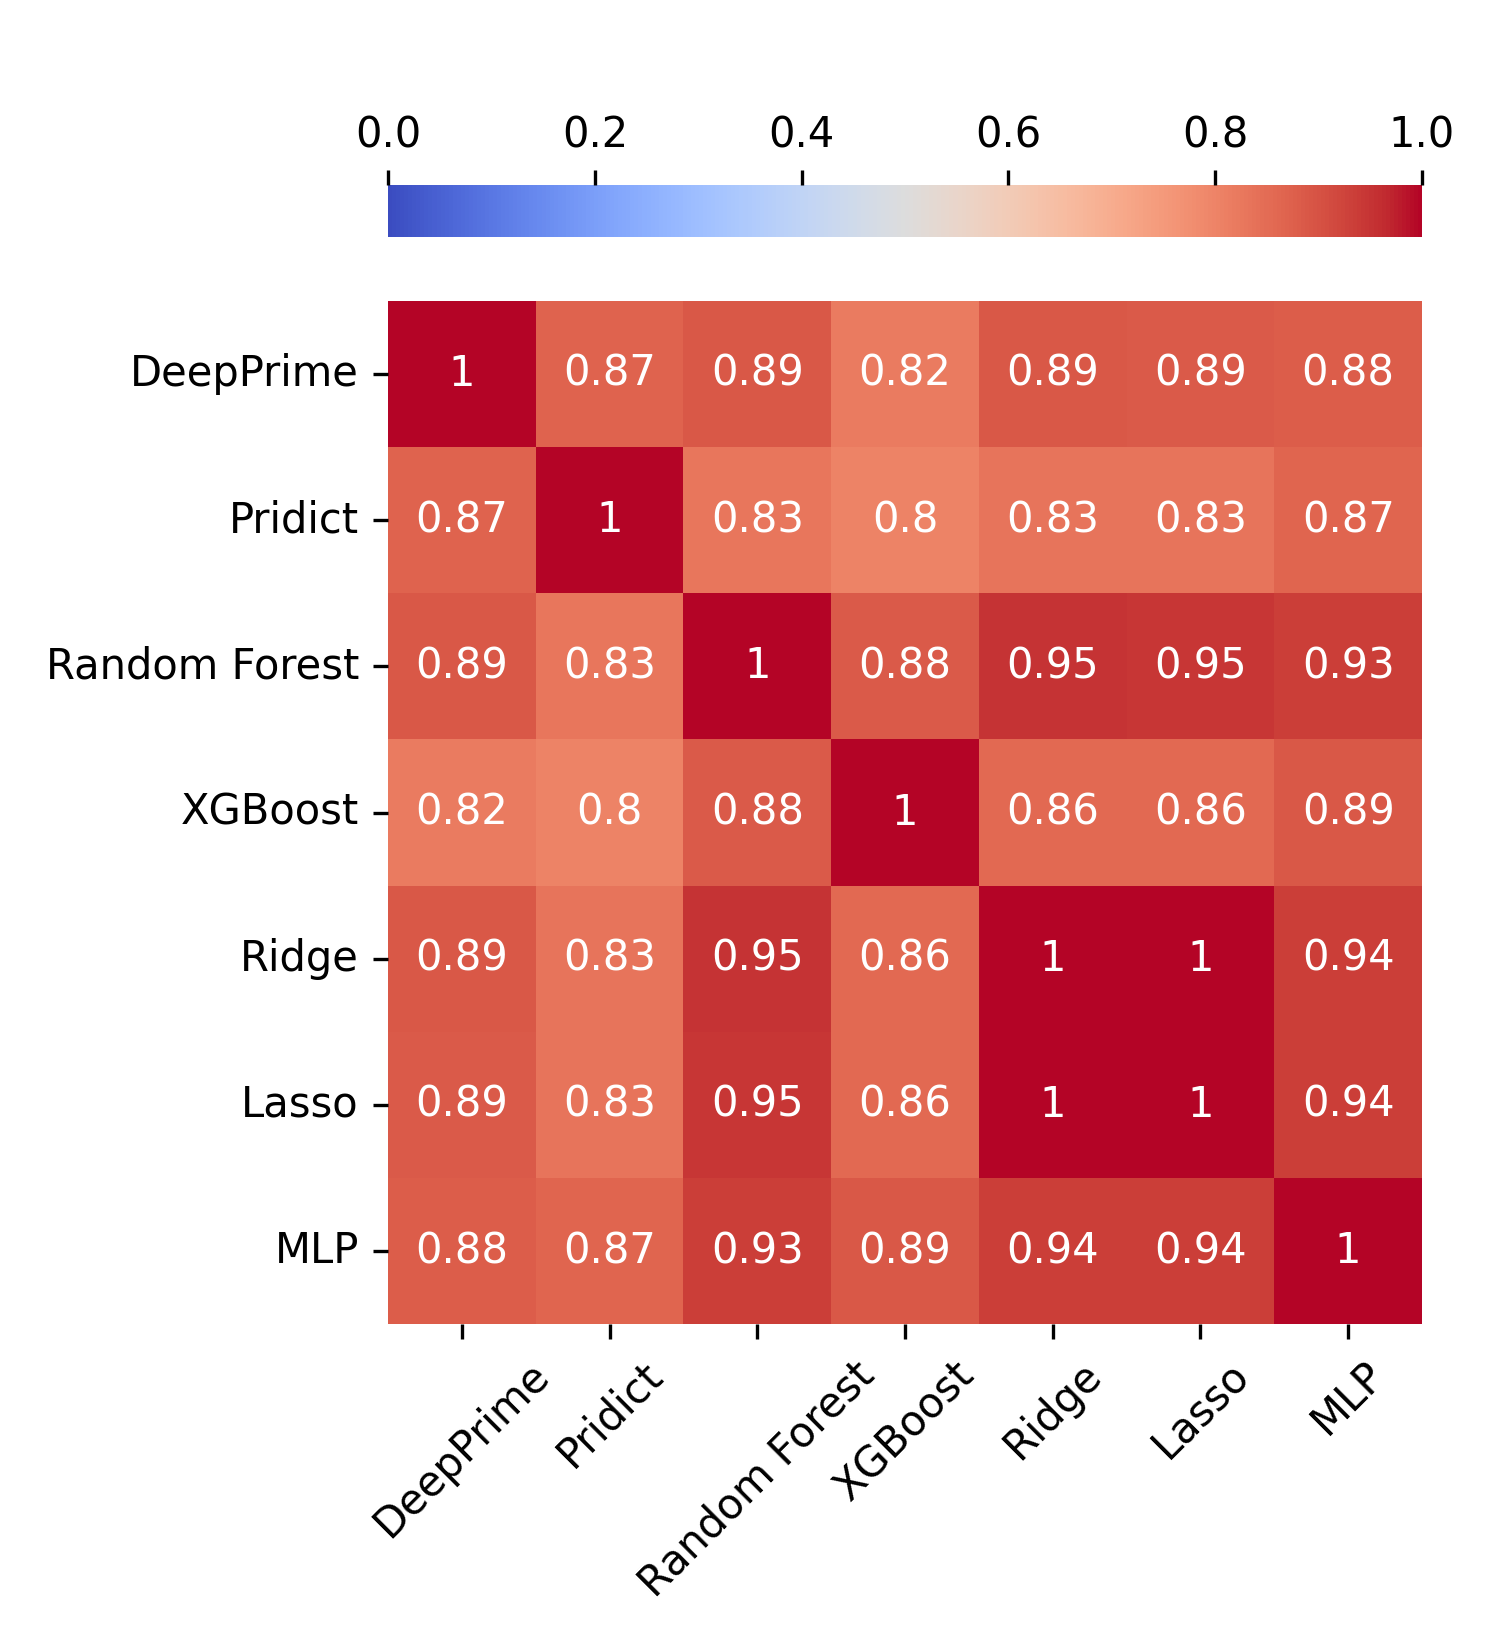
\includegraphics[width=0.49\textwidth]{error_correlation_pd-k562-pe2_pearson.png}
        % \caption{Pearson Correlation of the Error of the Individual Models}
        \label{fig:pearson-correlation-k562-pe2}
    }%
    \subfigure[][Spearman Correlation]{
        \centering
        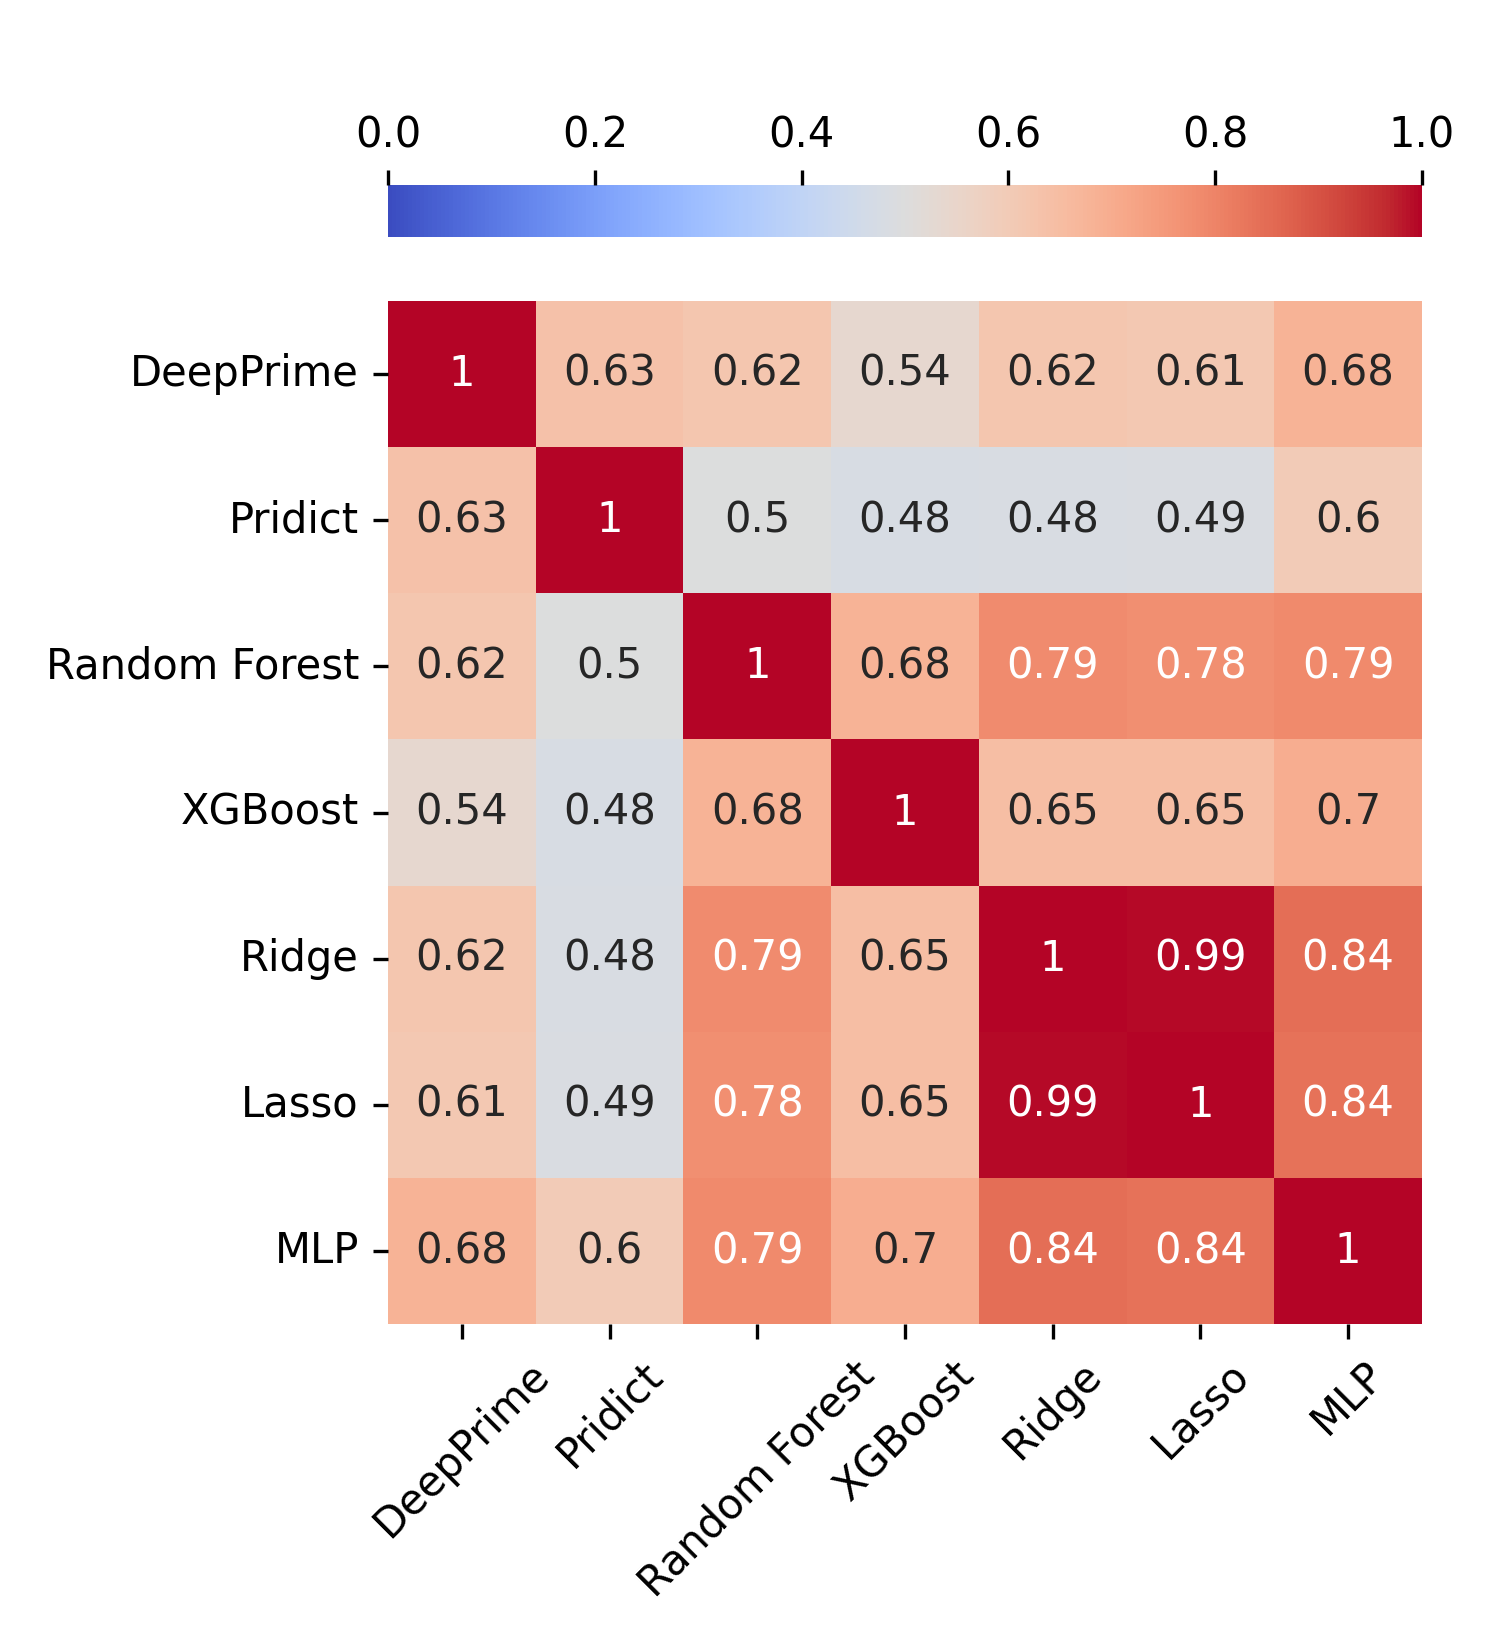
\includegraphics[width=0.49\textwidth]{error_correlation_pd-k562-pe2_spearman.png}
        % \caption{Spearman Correlation of the Error of the Individual Models}
        \label{fig:spearman-correlation-k562-pe2}
    }
    \caption[Error Analysis of the Individual Models on PRIDICT K562 PE2 dataset]{Error Analysis of the Individual Models on the PRIDICT K562 PE2 dataset. \textbf{(a)}, \textbf{(b)}, and \textbf{(c)} are the same as \autoref{fig:error-analysis-adv-pe2}.}
    \label{fig:error-analysis-k562-pe2}
\end{figure}
\newpage

\begin{figure}[!htb]
    \centering
    \subfigure[][Error Distribution]{
        \centering
        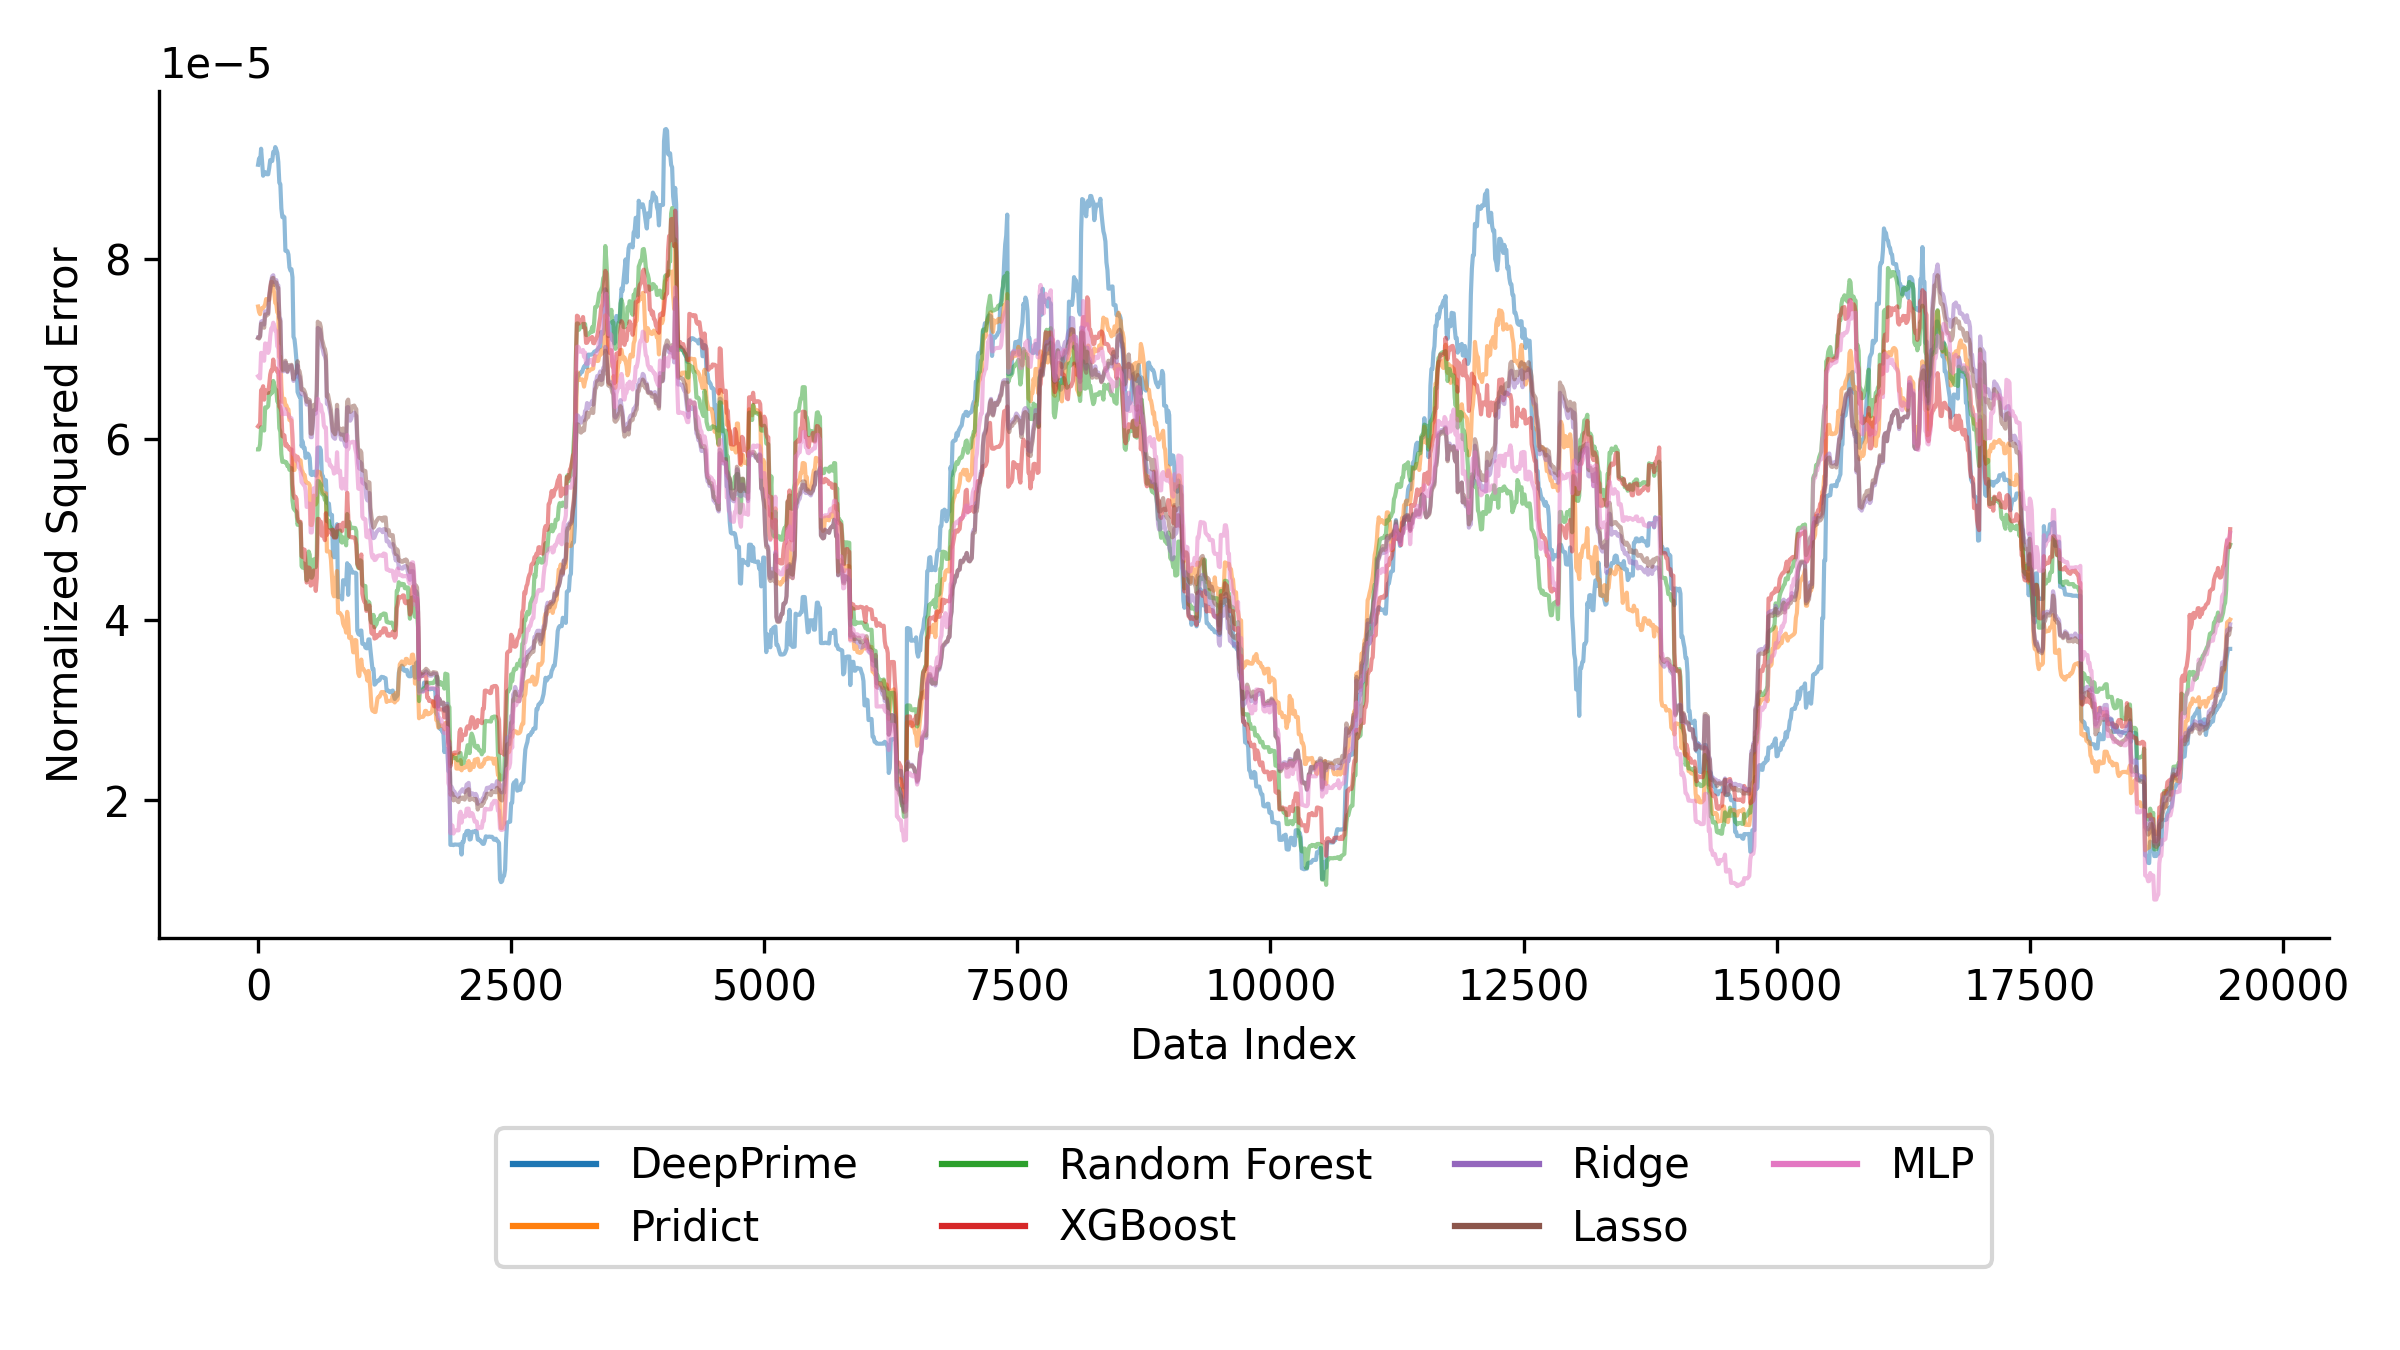
\includegraphics[width=\textwidth]{error_comparison_pd-k562mlh1dn-pe2.png}
        % \caption{Error Distribution of the Individual Models}
        \label{fig:error-distribution-k562mlh1dn-pe2}
    }
    \subfigure[][Pearson Correlation]{
        \centering
        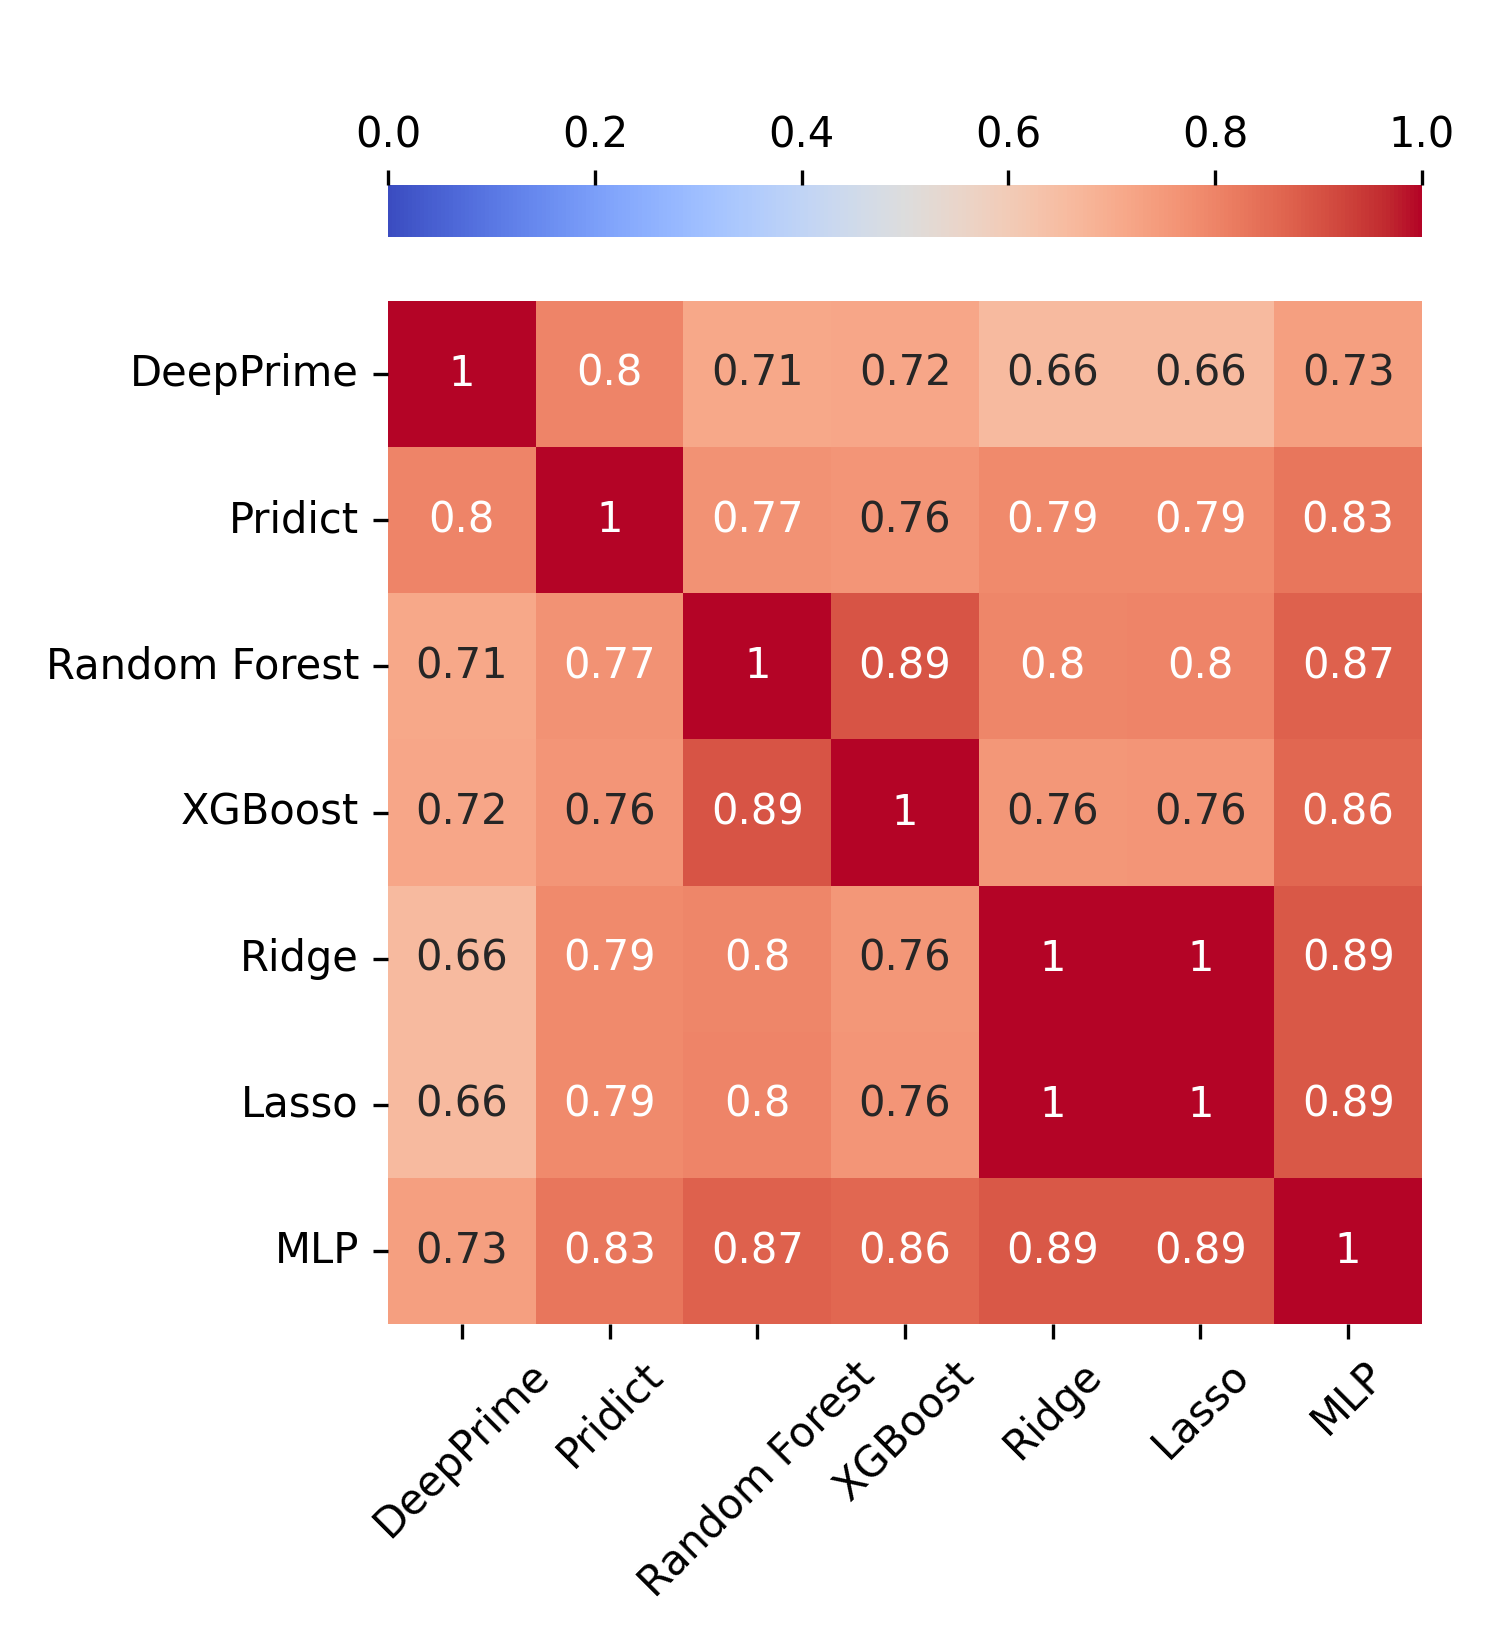
\includegraphics[width=0.49\textwidth]{error_correlation_pd-k562mlh1dn-pe2_pearson.png}
        % \caption{Pearson Correlation of the Error of the Individual Models}
        \label{fig:pearson-correlation-k562mlh1dn-pe2}
    }%
    \subfigure[][Spearman Correlation]{
        \centering
        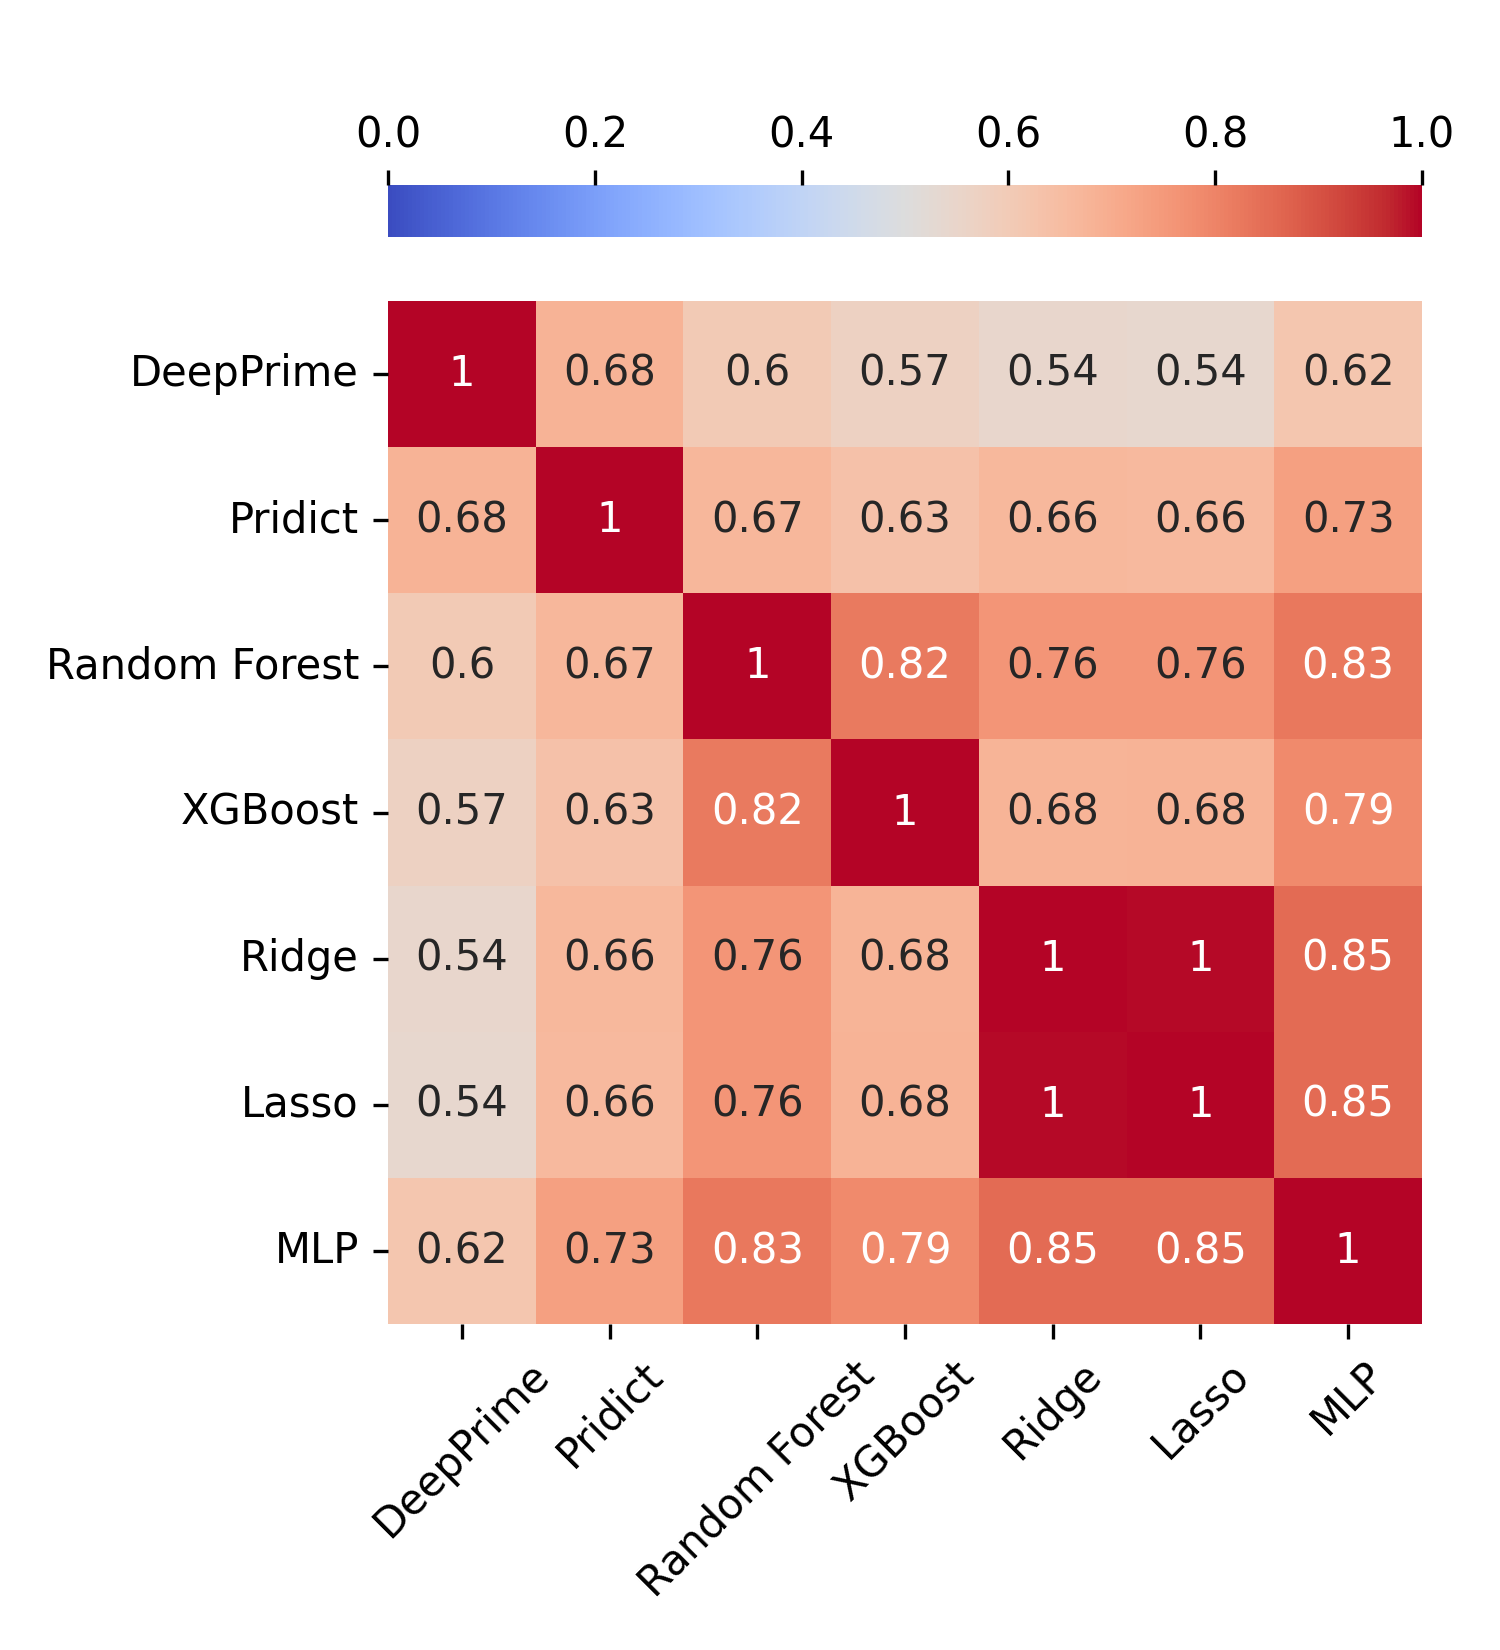
\includegraphics[width=0.49\textwidth]{error_correlation_pd-k562mlh1dn-pe2_spearman.png}
        % \caption{Spearman Correlation of the Error of the Individual Models}
        \label{fig:spearman-correlation-k562mlh1dn-pe2}
    }
    \caption[Error Analysis of the Individual Models on PRIDICT K562 MLH1 DN PE2 dataset]{Error Analysis of the Individual Models on the PRIDICT K562 MLH1 DN PE2 dataset. \textbf{(a)}, \textbf{(b)}, and \textbf{(c)} are the same as \autoref{fig:error-analysis-adv-pe2}.}
    \label{fig:error-analysis-k562mlh1dn-pe2}
\end{figure}


\newpage

\section{Additional Figures for 1bp SHAP Analysis}
\label{appendix:shap-1bp-pridict}

During \autoref{sec:attention_analysis}, we discussed how SHAP analysis placed very little importance in the base pair to delete, contradicting the possible findings of the transformer models. To further verify this, the SHAP analysis was conducted on the 1bp edits on four other big datasets from PRIDICT. The results are shown in \autoref{fig:shap-1bp-adv-pe2}, \autoref{fig:shap-1bp-hek293t-pe2}, \autoref{fig:shap-1bp-k562-pe2}, and \autoref{fig:shap-1bp-k562mlh1dn-pe2}. The results are consistent with the findings in \autoref{sec:attention_analysis}, showing that the base pair to delete is not considered important for the editing efficiency by the XGBoost model.

\begin{figure}[!htb]
    \centering
    \subfigure[Substitution]{
        \centering
        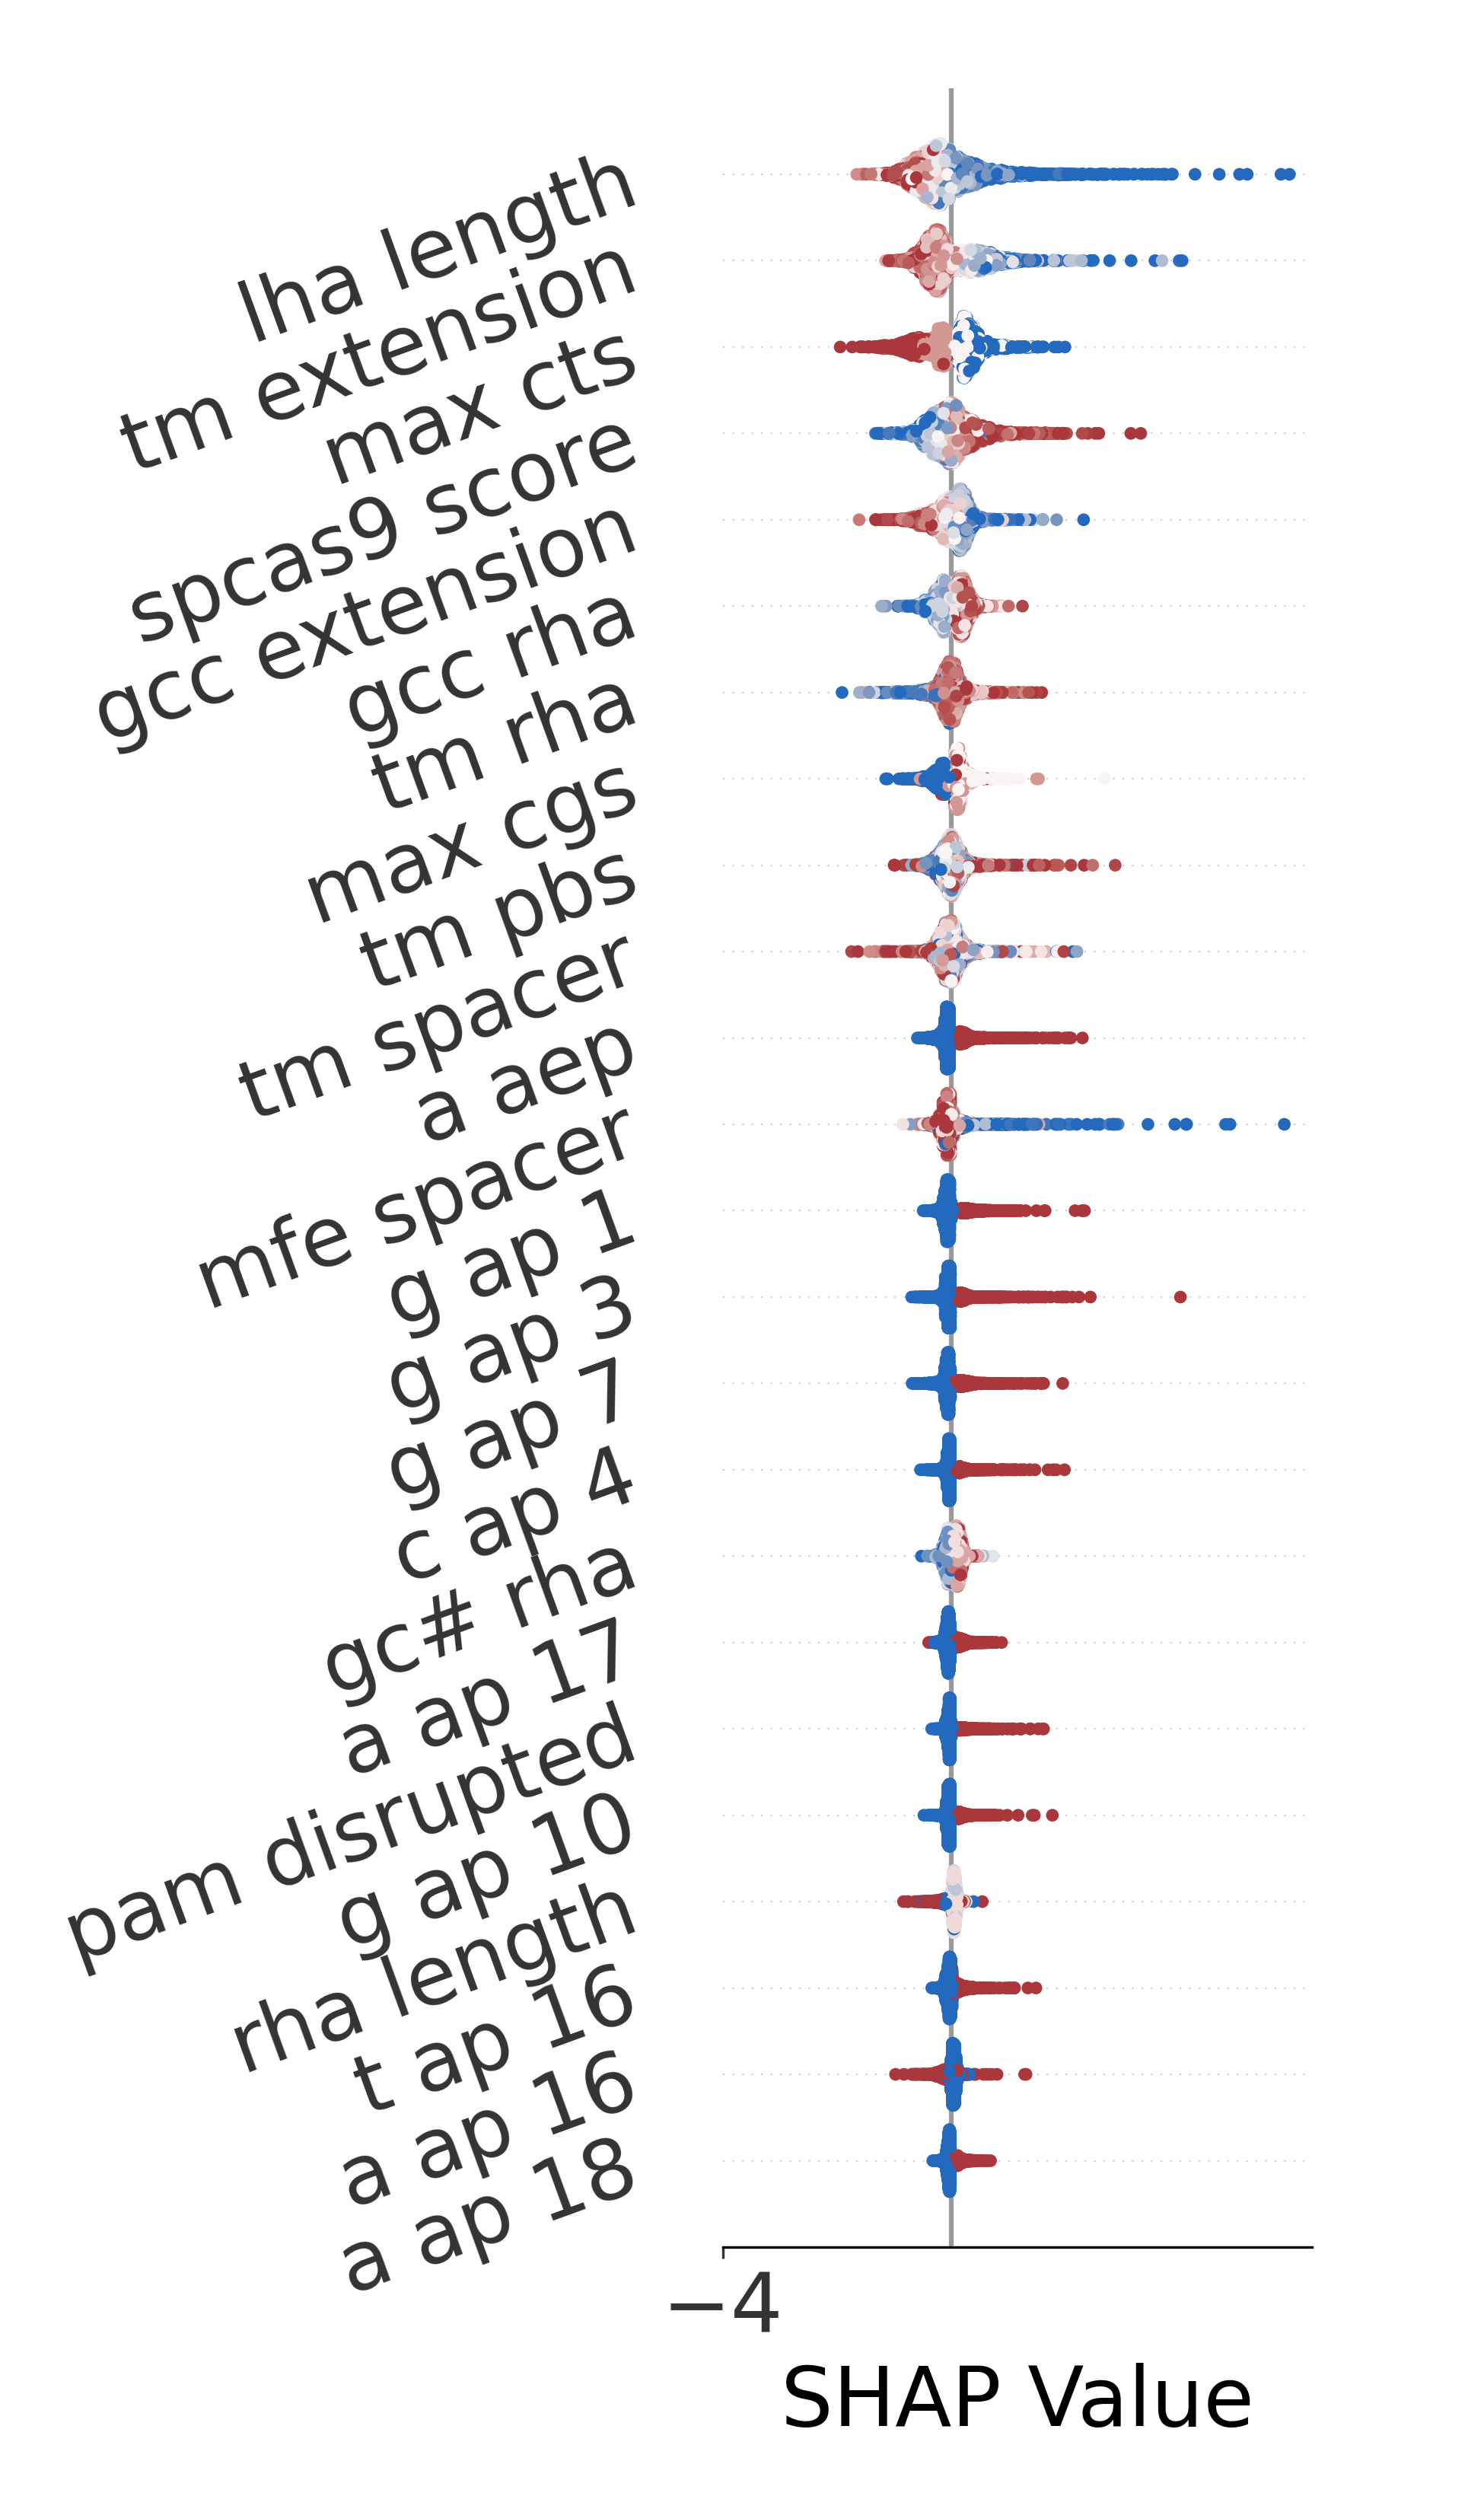
\includegraphics[width=0.33\textwidth]{shap_1bp-pd-adv-pe2-replace.png}
        \label{fig:shap-1bp-adv-pe2-replace}
    }%
    \subfigure[Insertion]{
        \centering
        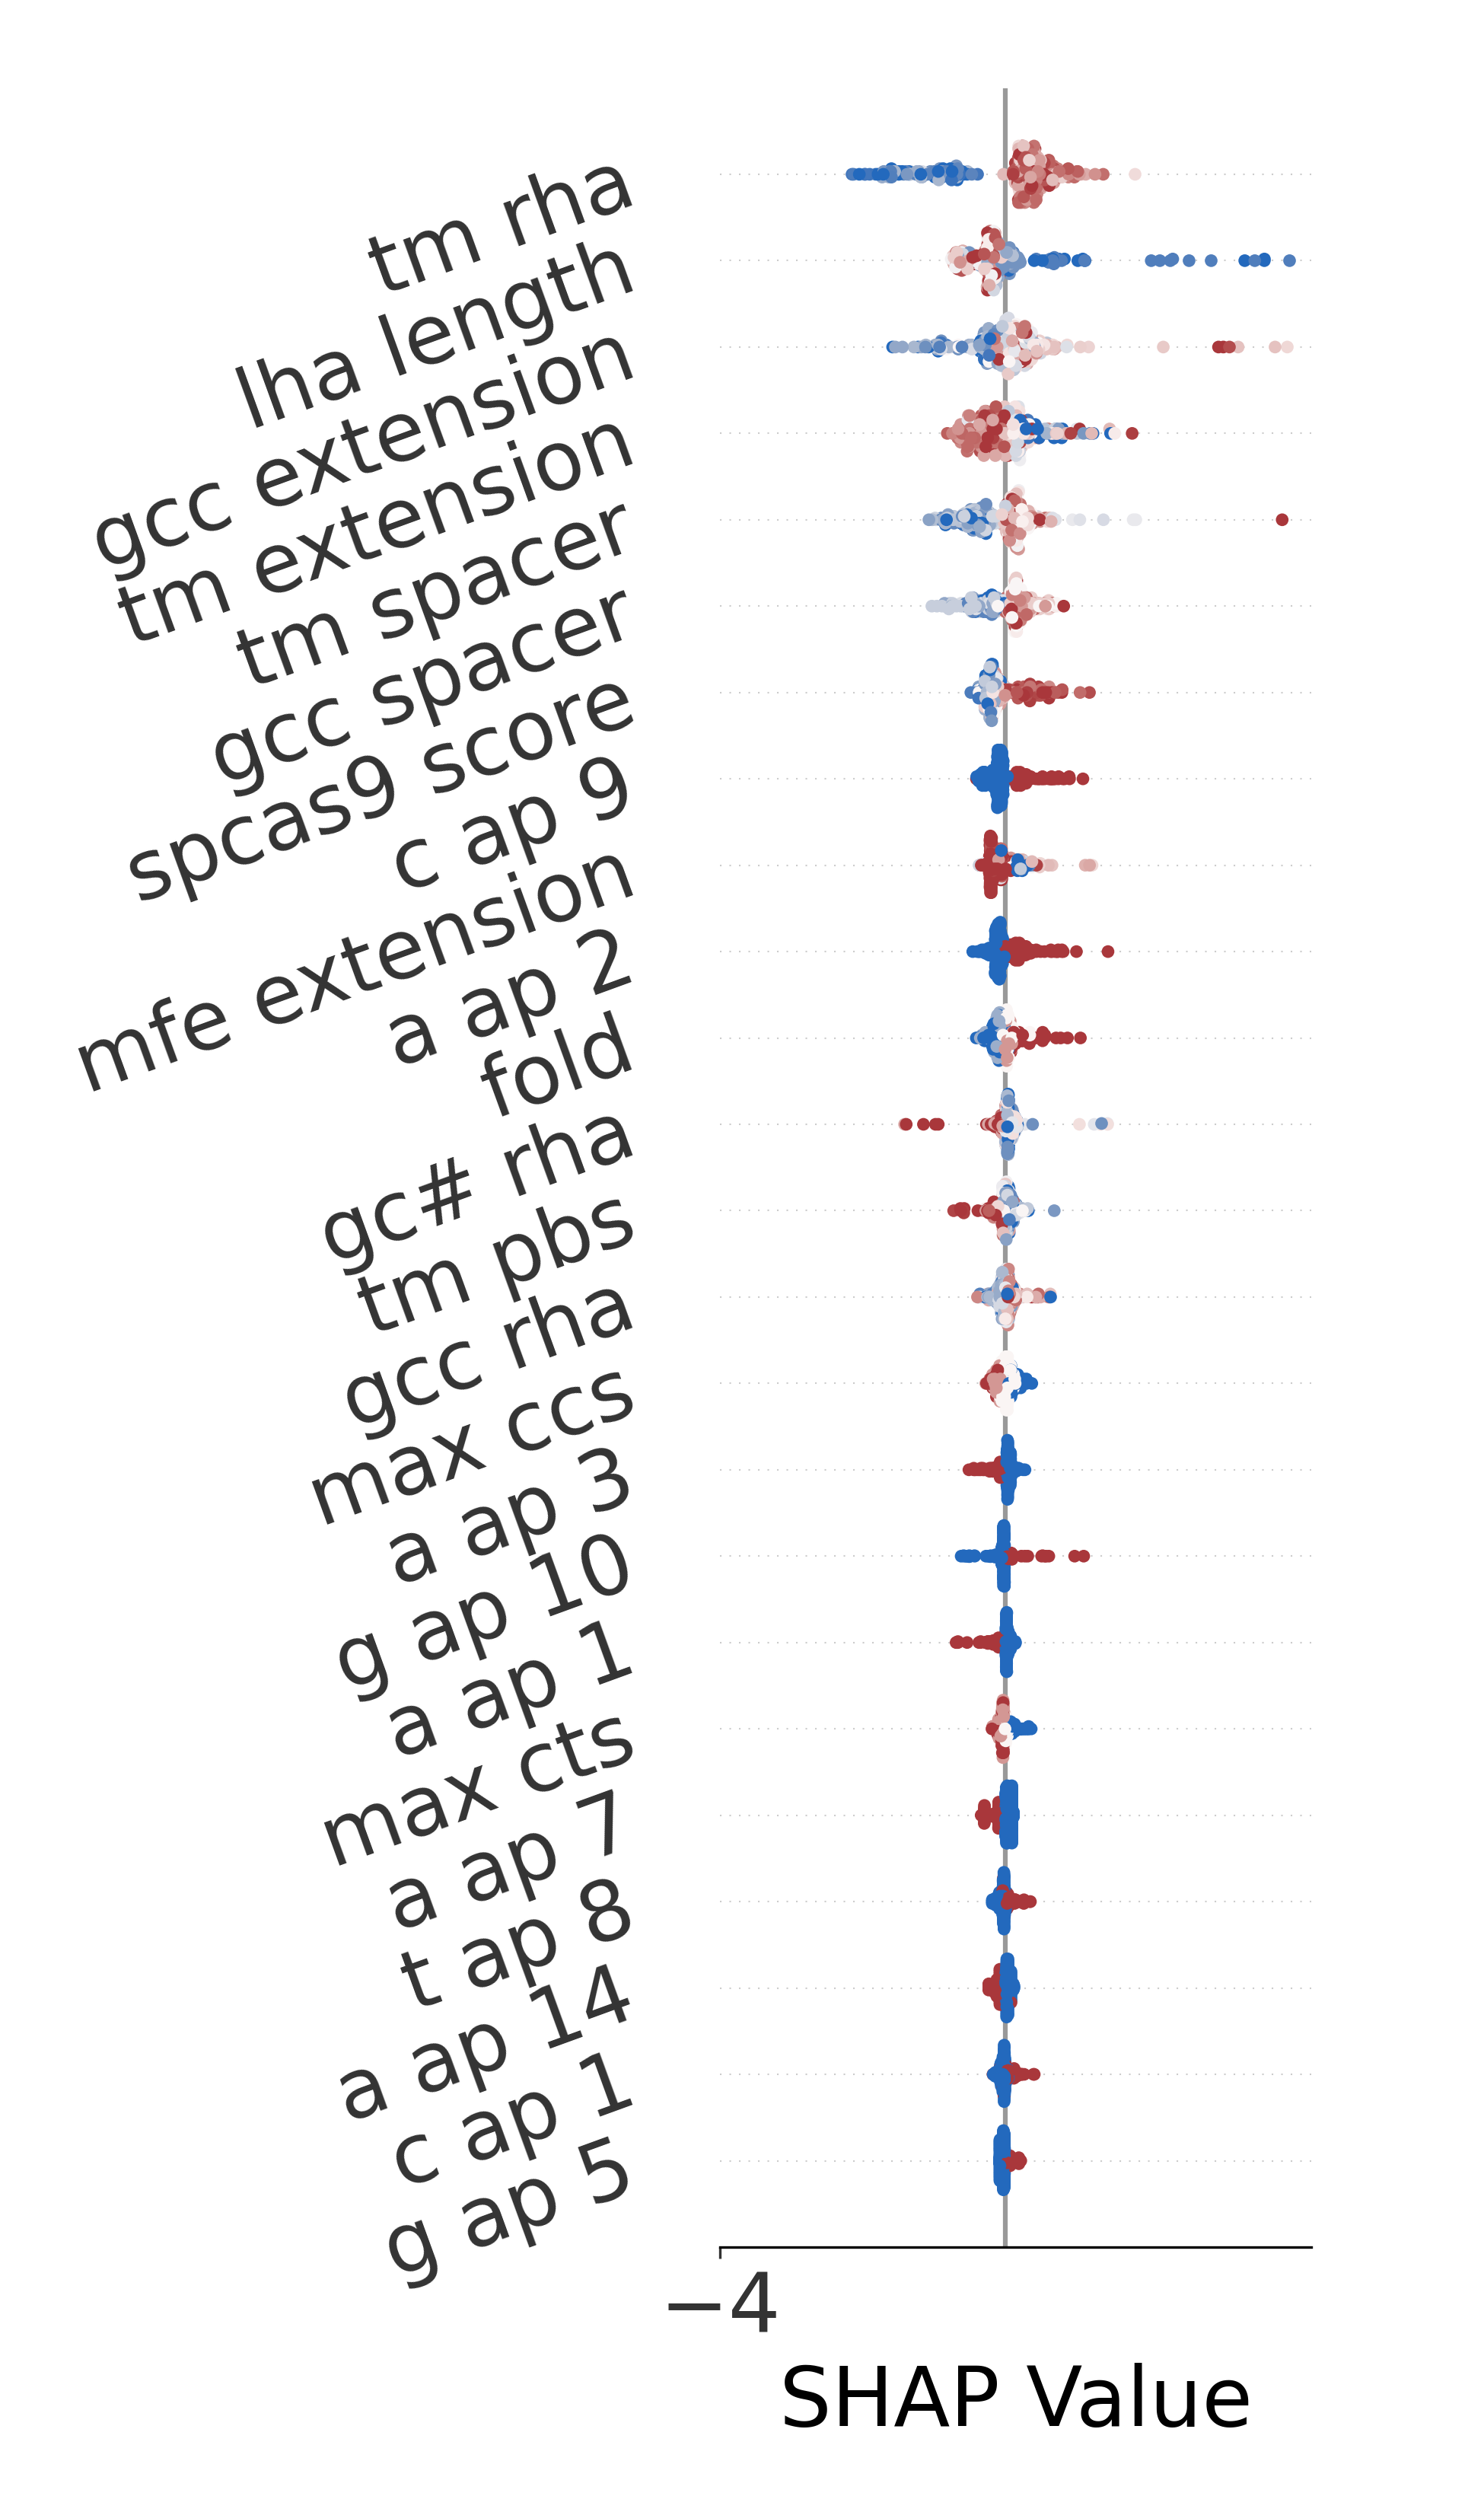
\includegraphics[width=0.33\textwidth]{shap_1bp-pd-adv-pe2-insert.png}
        \label{fig:shap-1bp-adv-pe2-insert}
    }%
    \subfigure[Deletion]{
        \centering
        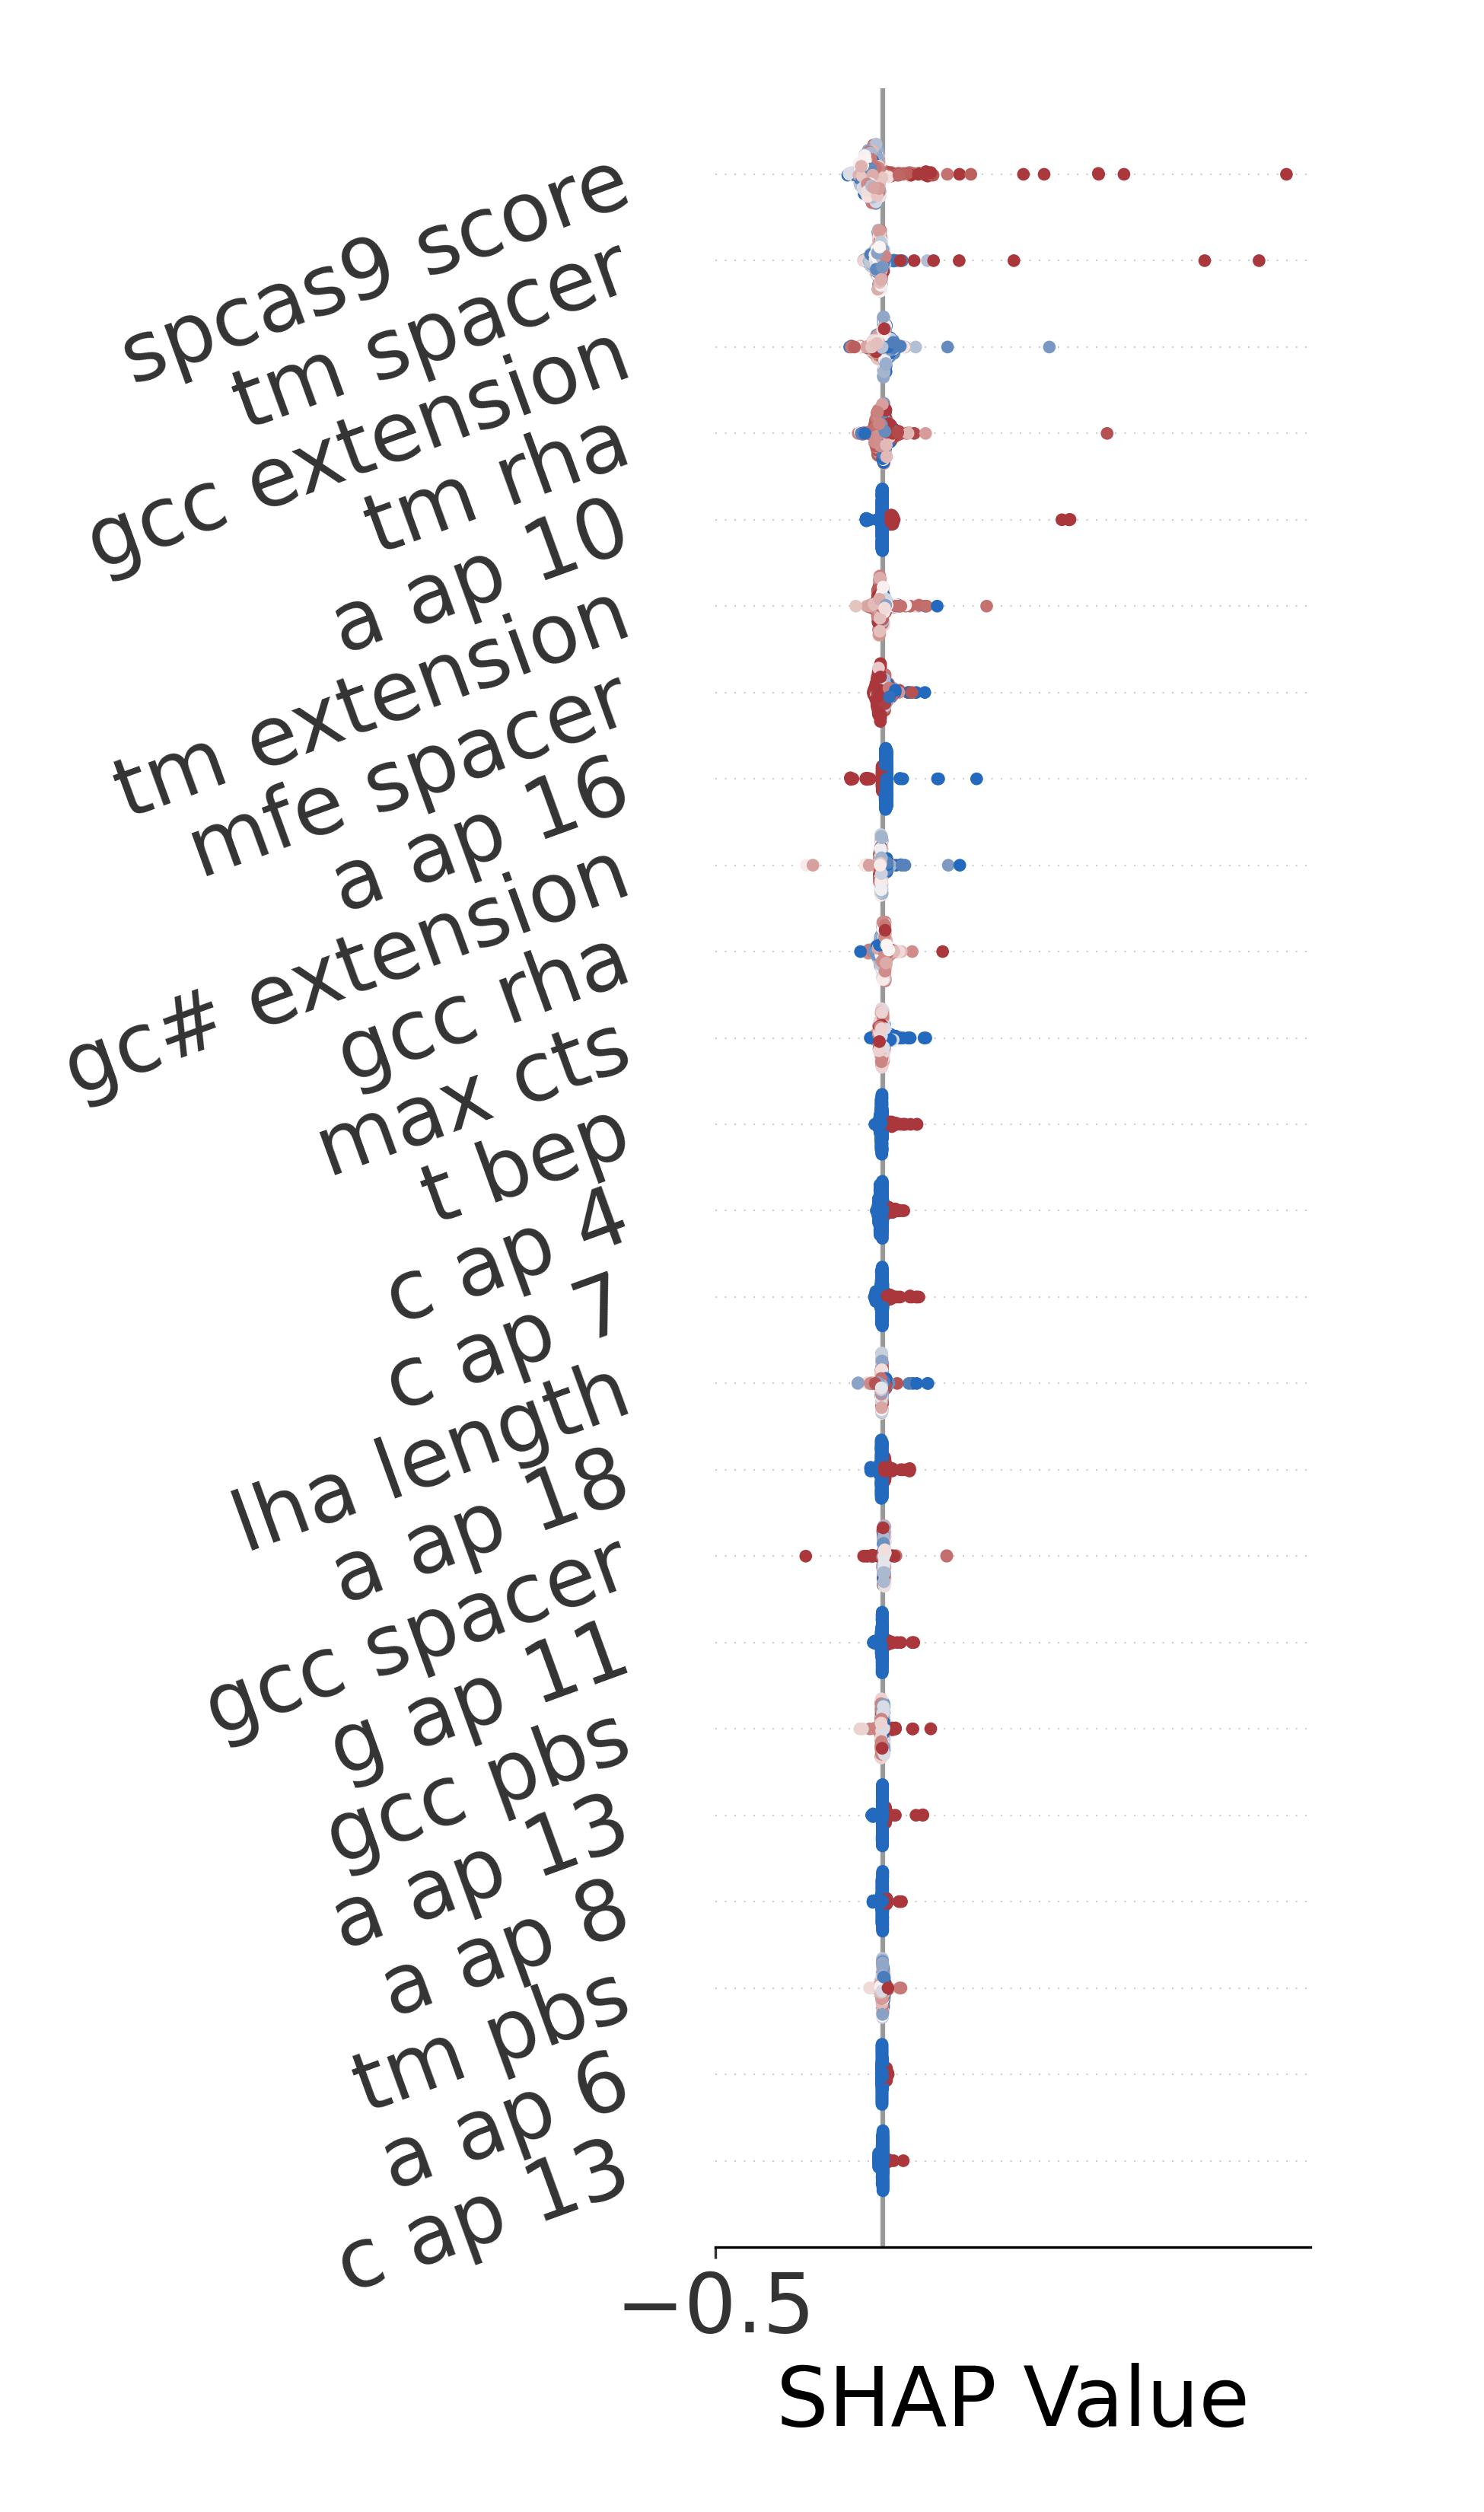
\includegraphics[width=0.33\textwidth]{shap_1bp-pd-adv-pe2-delete.png}
        \label{fig:shap-1bp-adv-pe2-delete}
    }
    \caption[SHAP Analysis of 1bp Edits on PRIDICT Adv PE2 Dataset]{SHAP Analysis of 1bp Edits on the PRIDICT Adv PE2 dataset. The SHAP values are calculated for the base pair to replace, insert, and delete. The SHAP values are averaged over all the examples in the dataset.}
    \label{fig:shap-1bp-adv-pe2}
\end{figure}

\begin{figure}[!htb]
    \centering
    \subfigure[Substitution]{
        \centering
        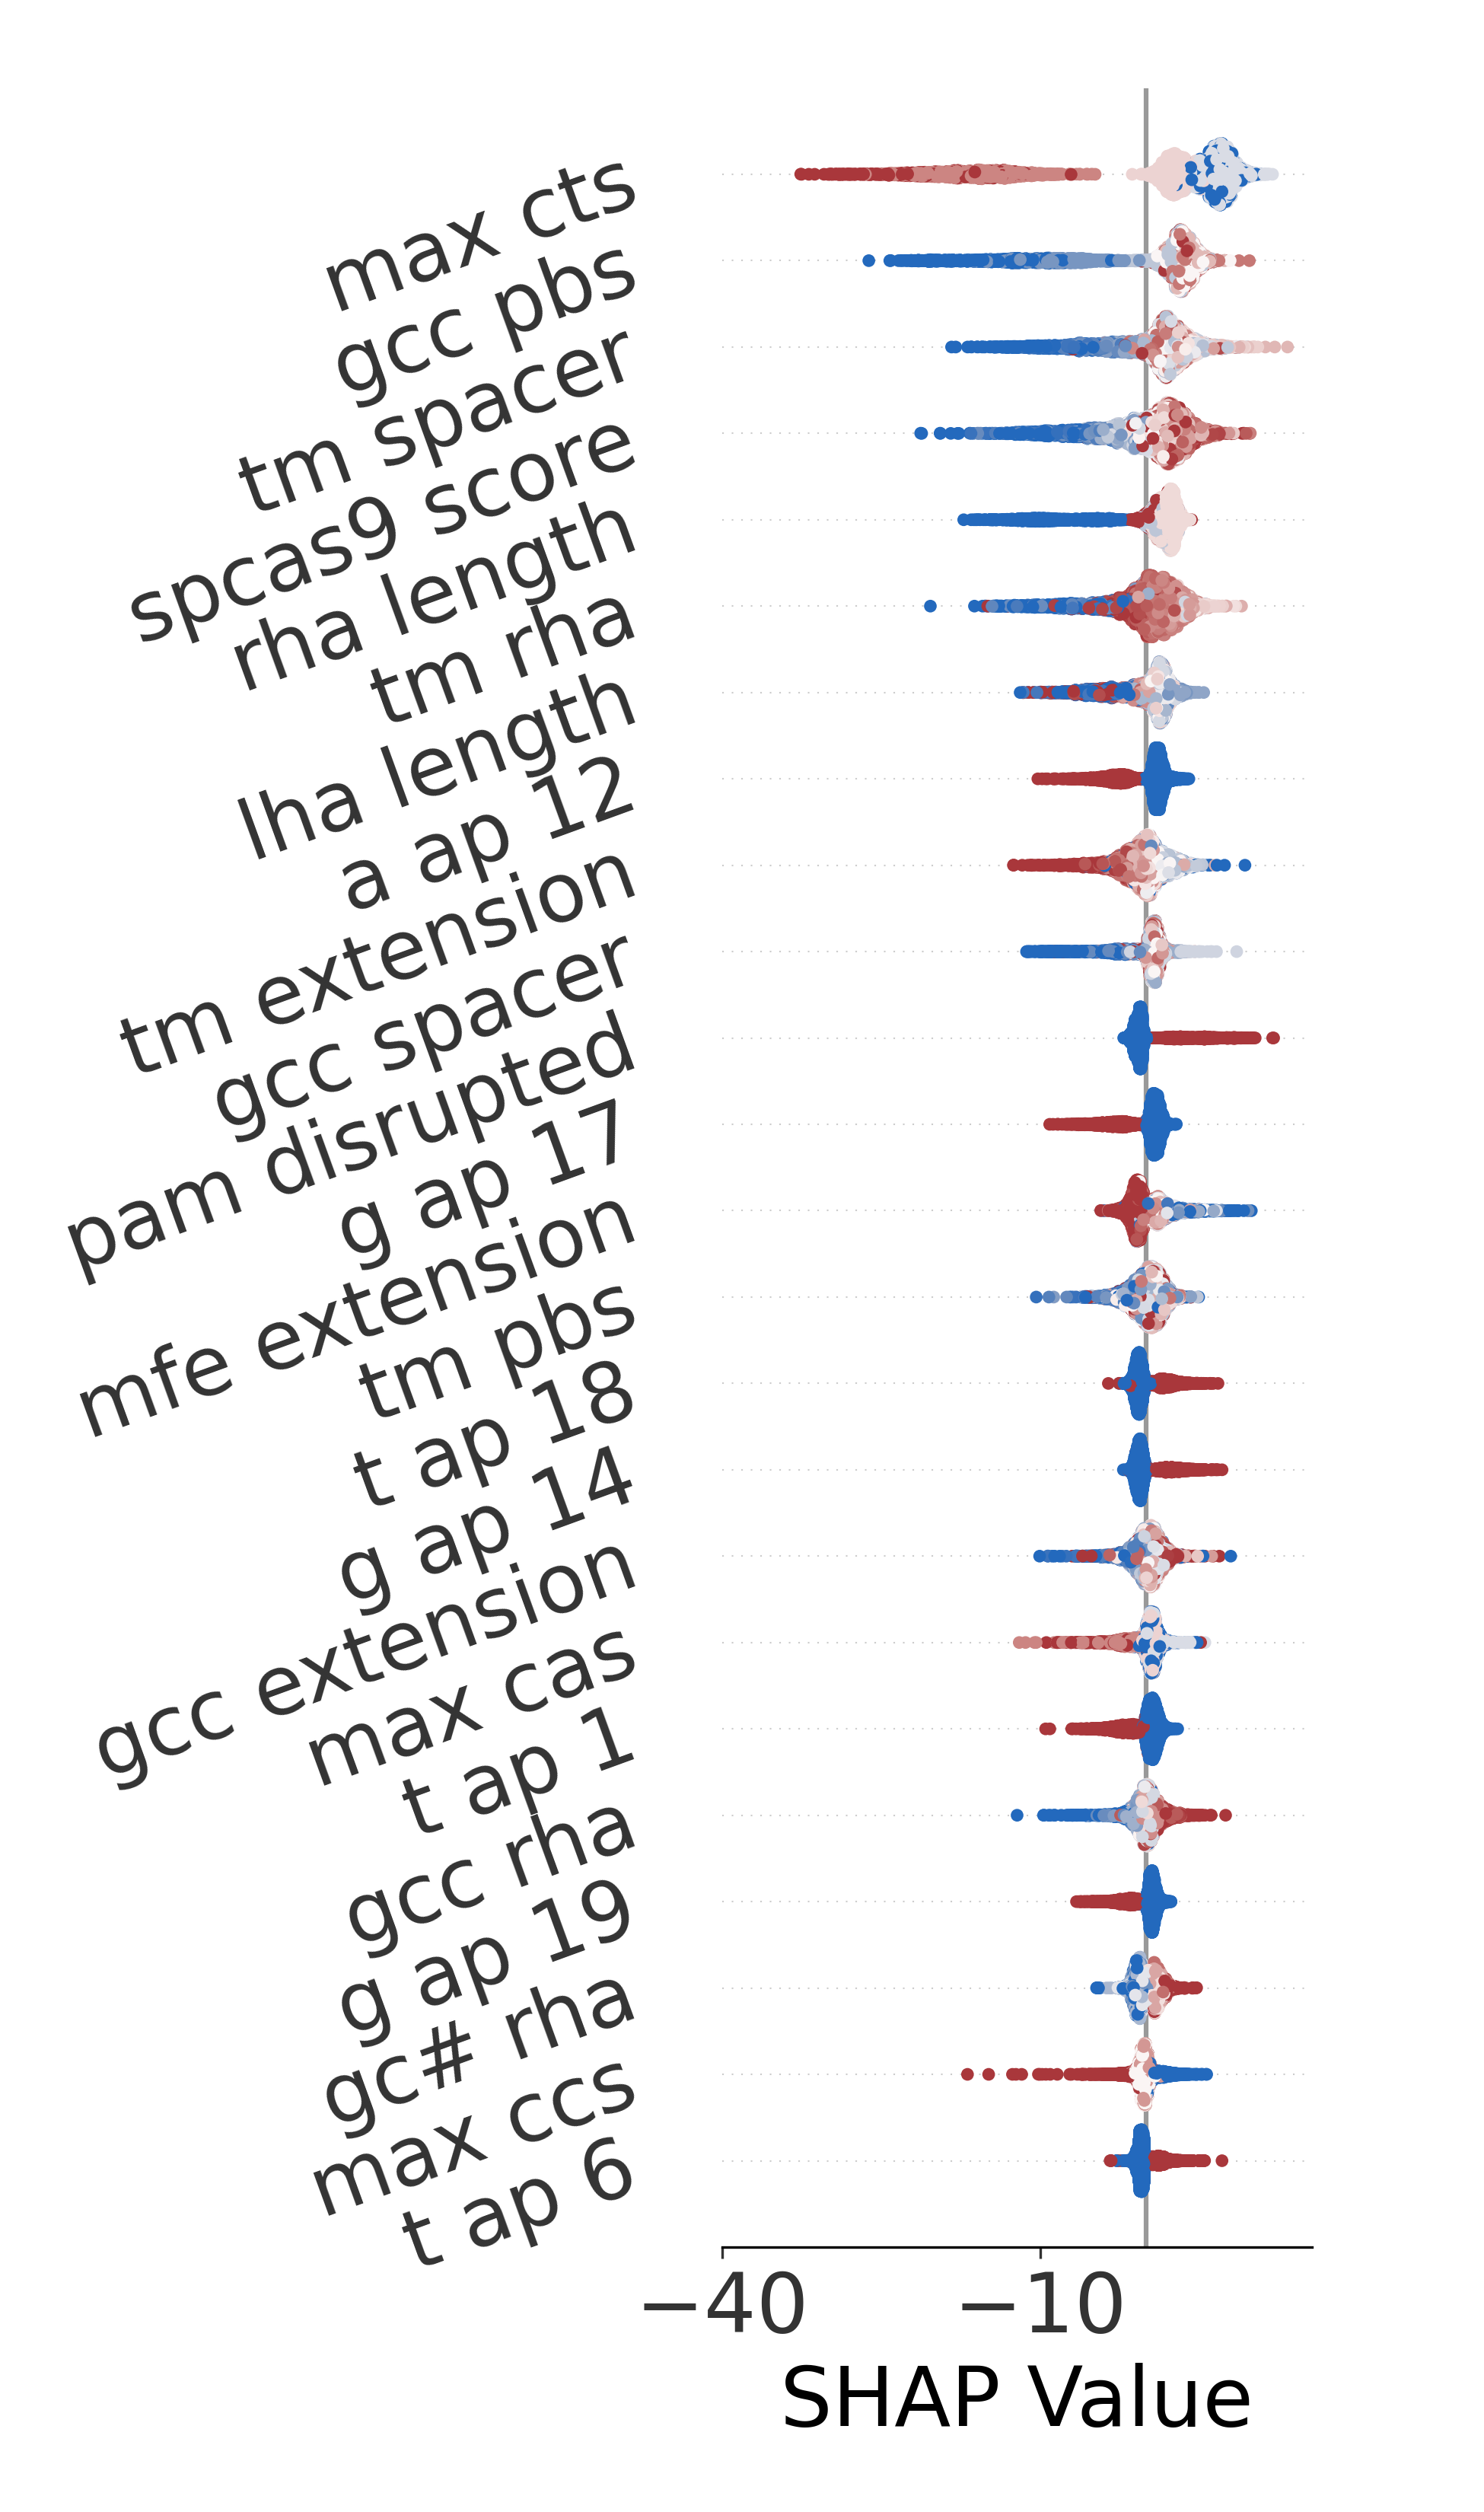
\includegraphics[width=0.33\textwidth]{shap_1bp-pd-hek293t-pe2-replace.png}
        \label{fig:shap-1bp-hek293t-pe2-replace}
    }%
    \subfigure[Insertion]{
        \centering
        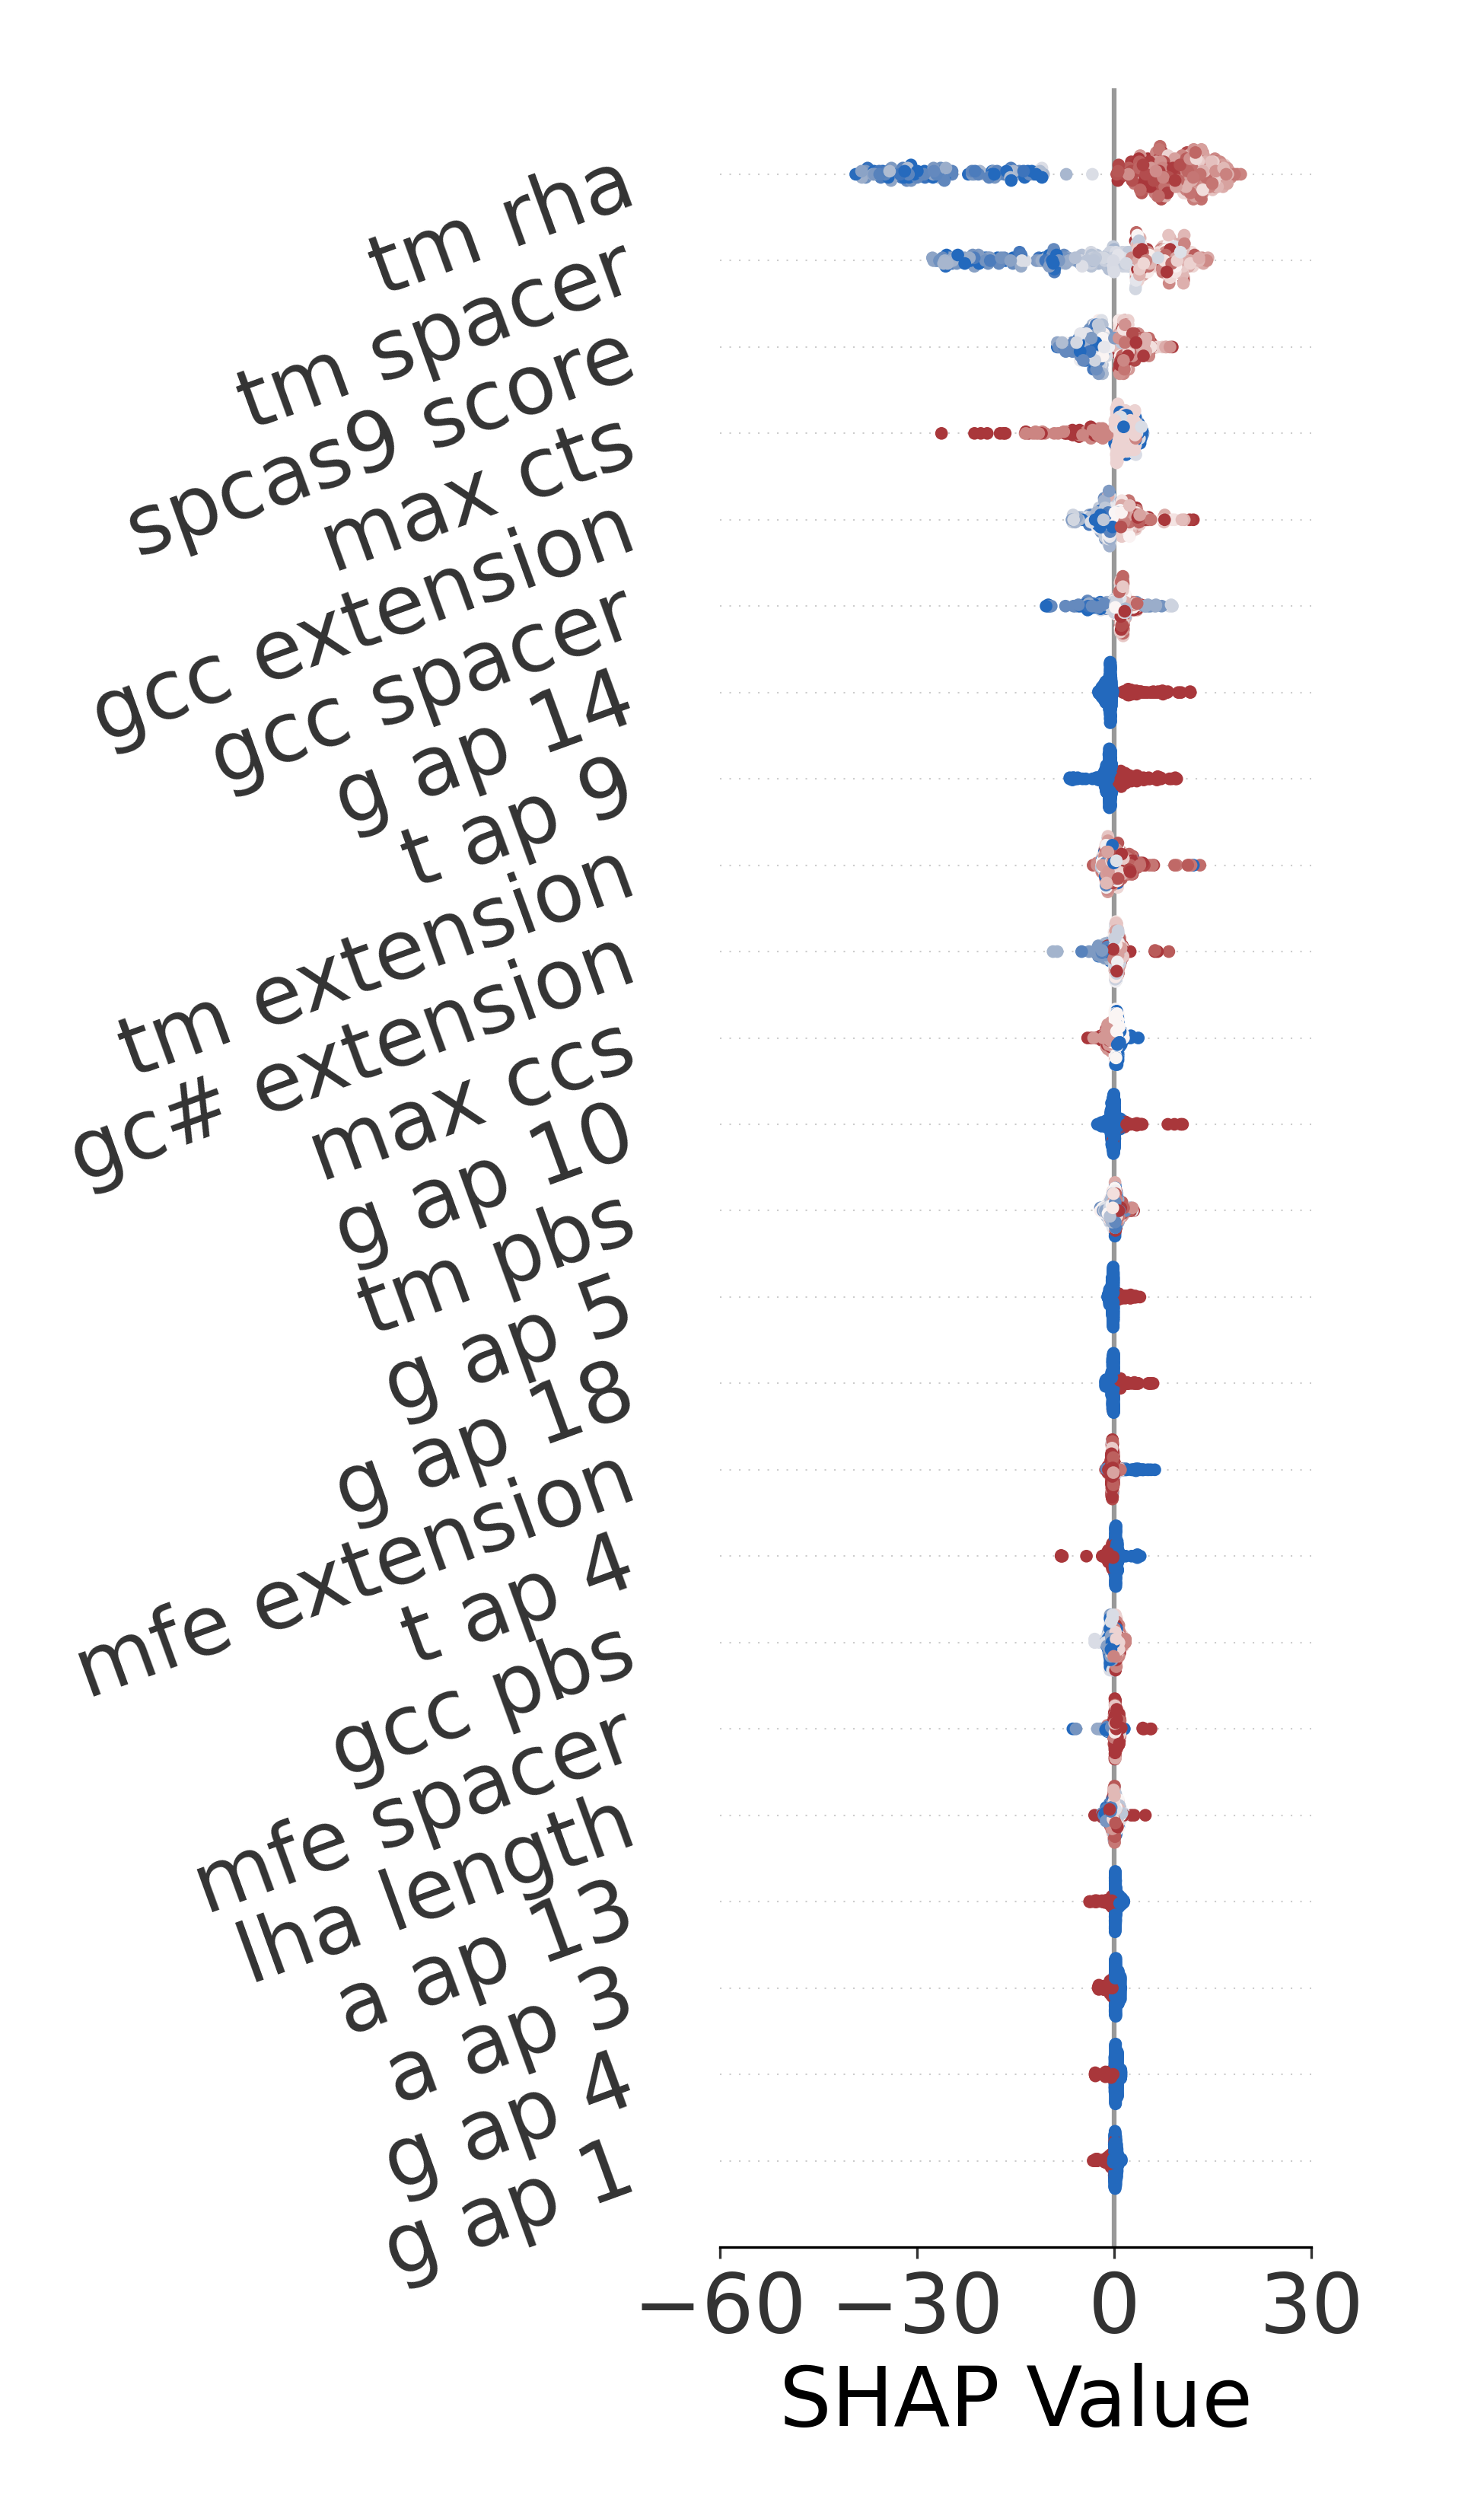
\includegraphics[width=0.33\textwidth]{shap_1bp-pd-hek293t-pe2-insert.png}
        \label{fig:shap-1bp-hek293t-pe2-insert}
    }%
    \subfigure[Deletion]{
        \centering
        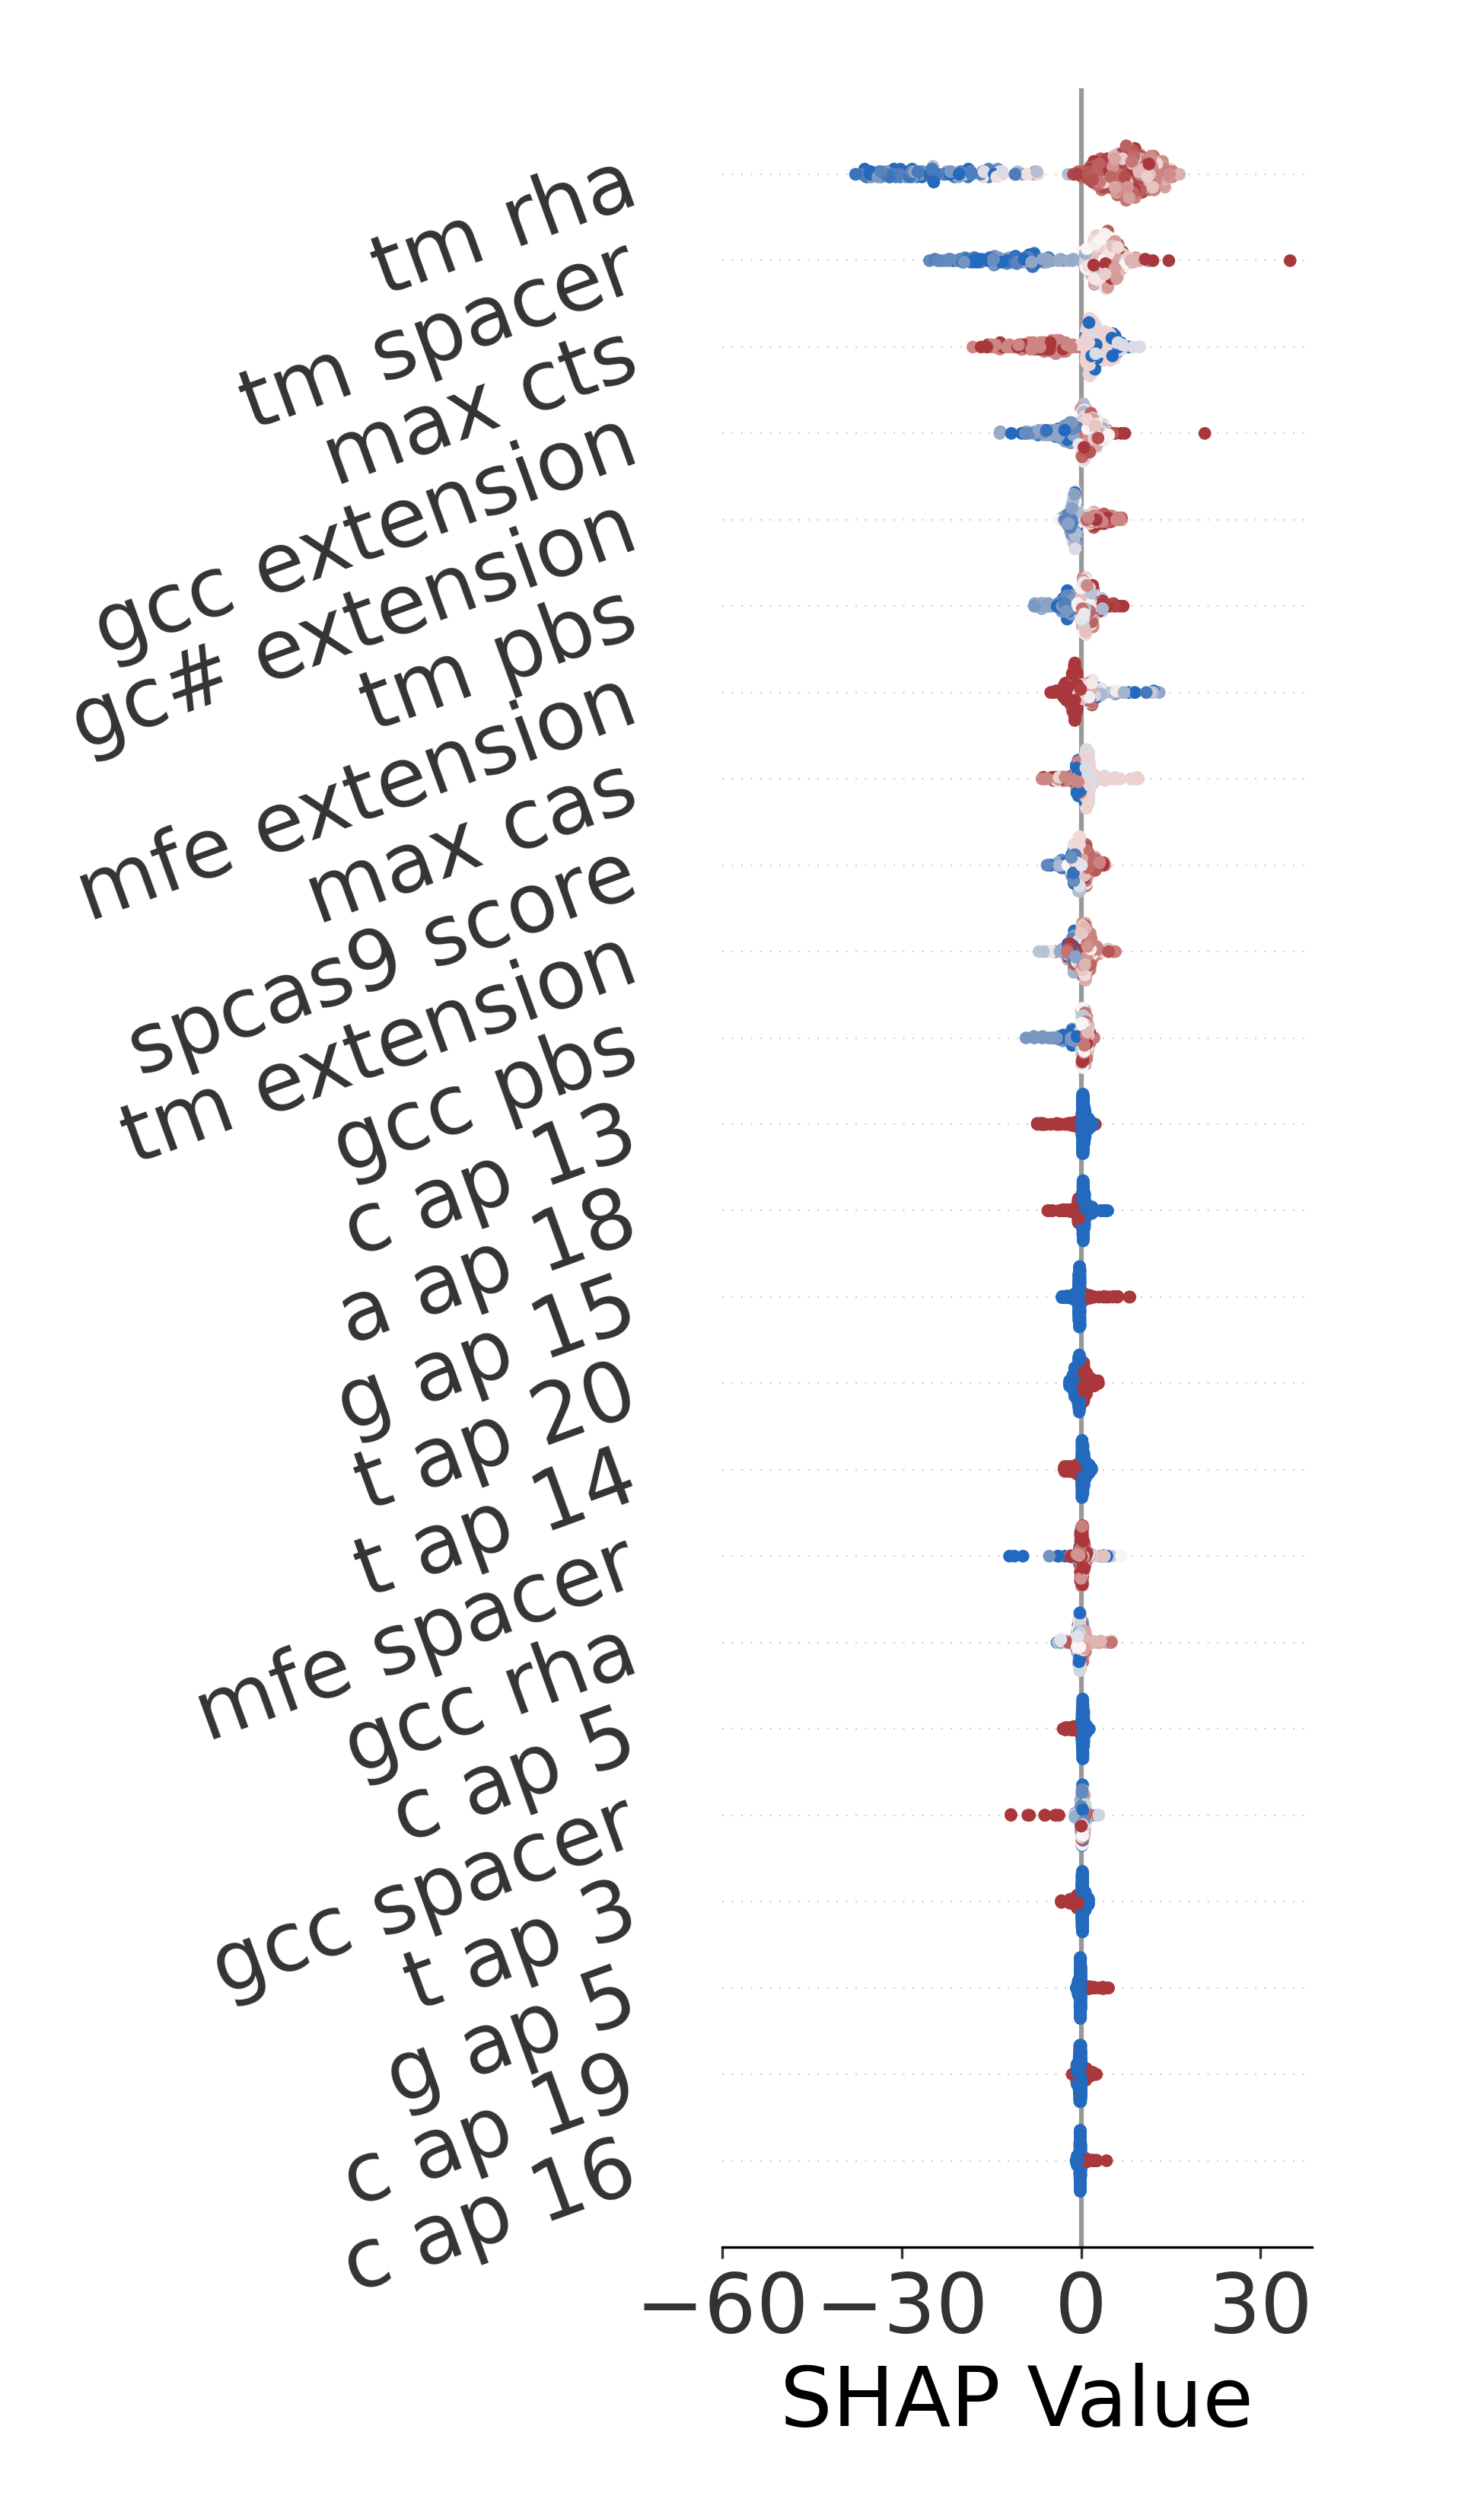
\includegraphics[width=0.33\textwidth]{shap_1bp-pd-hek293t-pe2-delete.png}
        \label{fig:shap-1bp-hek293t-pe2-delete}
    }
    \caption[SHAP Analysis of 1bp Edits on PRIDICT HEK293T PE2 Dataset]{SHAP Analysis of 1bp Edits on the PRIDICT HEK293T PE2 dataset. The SHAP values are calculated for the base pair to replace, insert, and delete. The SHAP values are averaged over all the examples in the dataset.}
    \label{fig:shap-1bp-hek293t-pe2}
\end{figure}

\begin{figure}[!htb]
    \centering
    \subfigure[Substitution]{
        \centering
        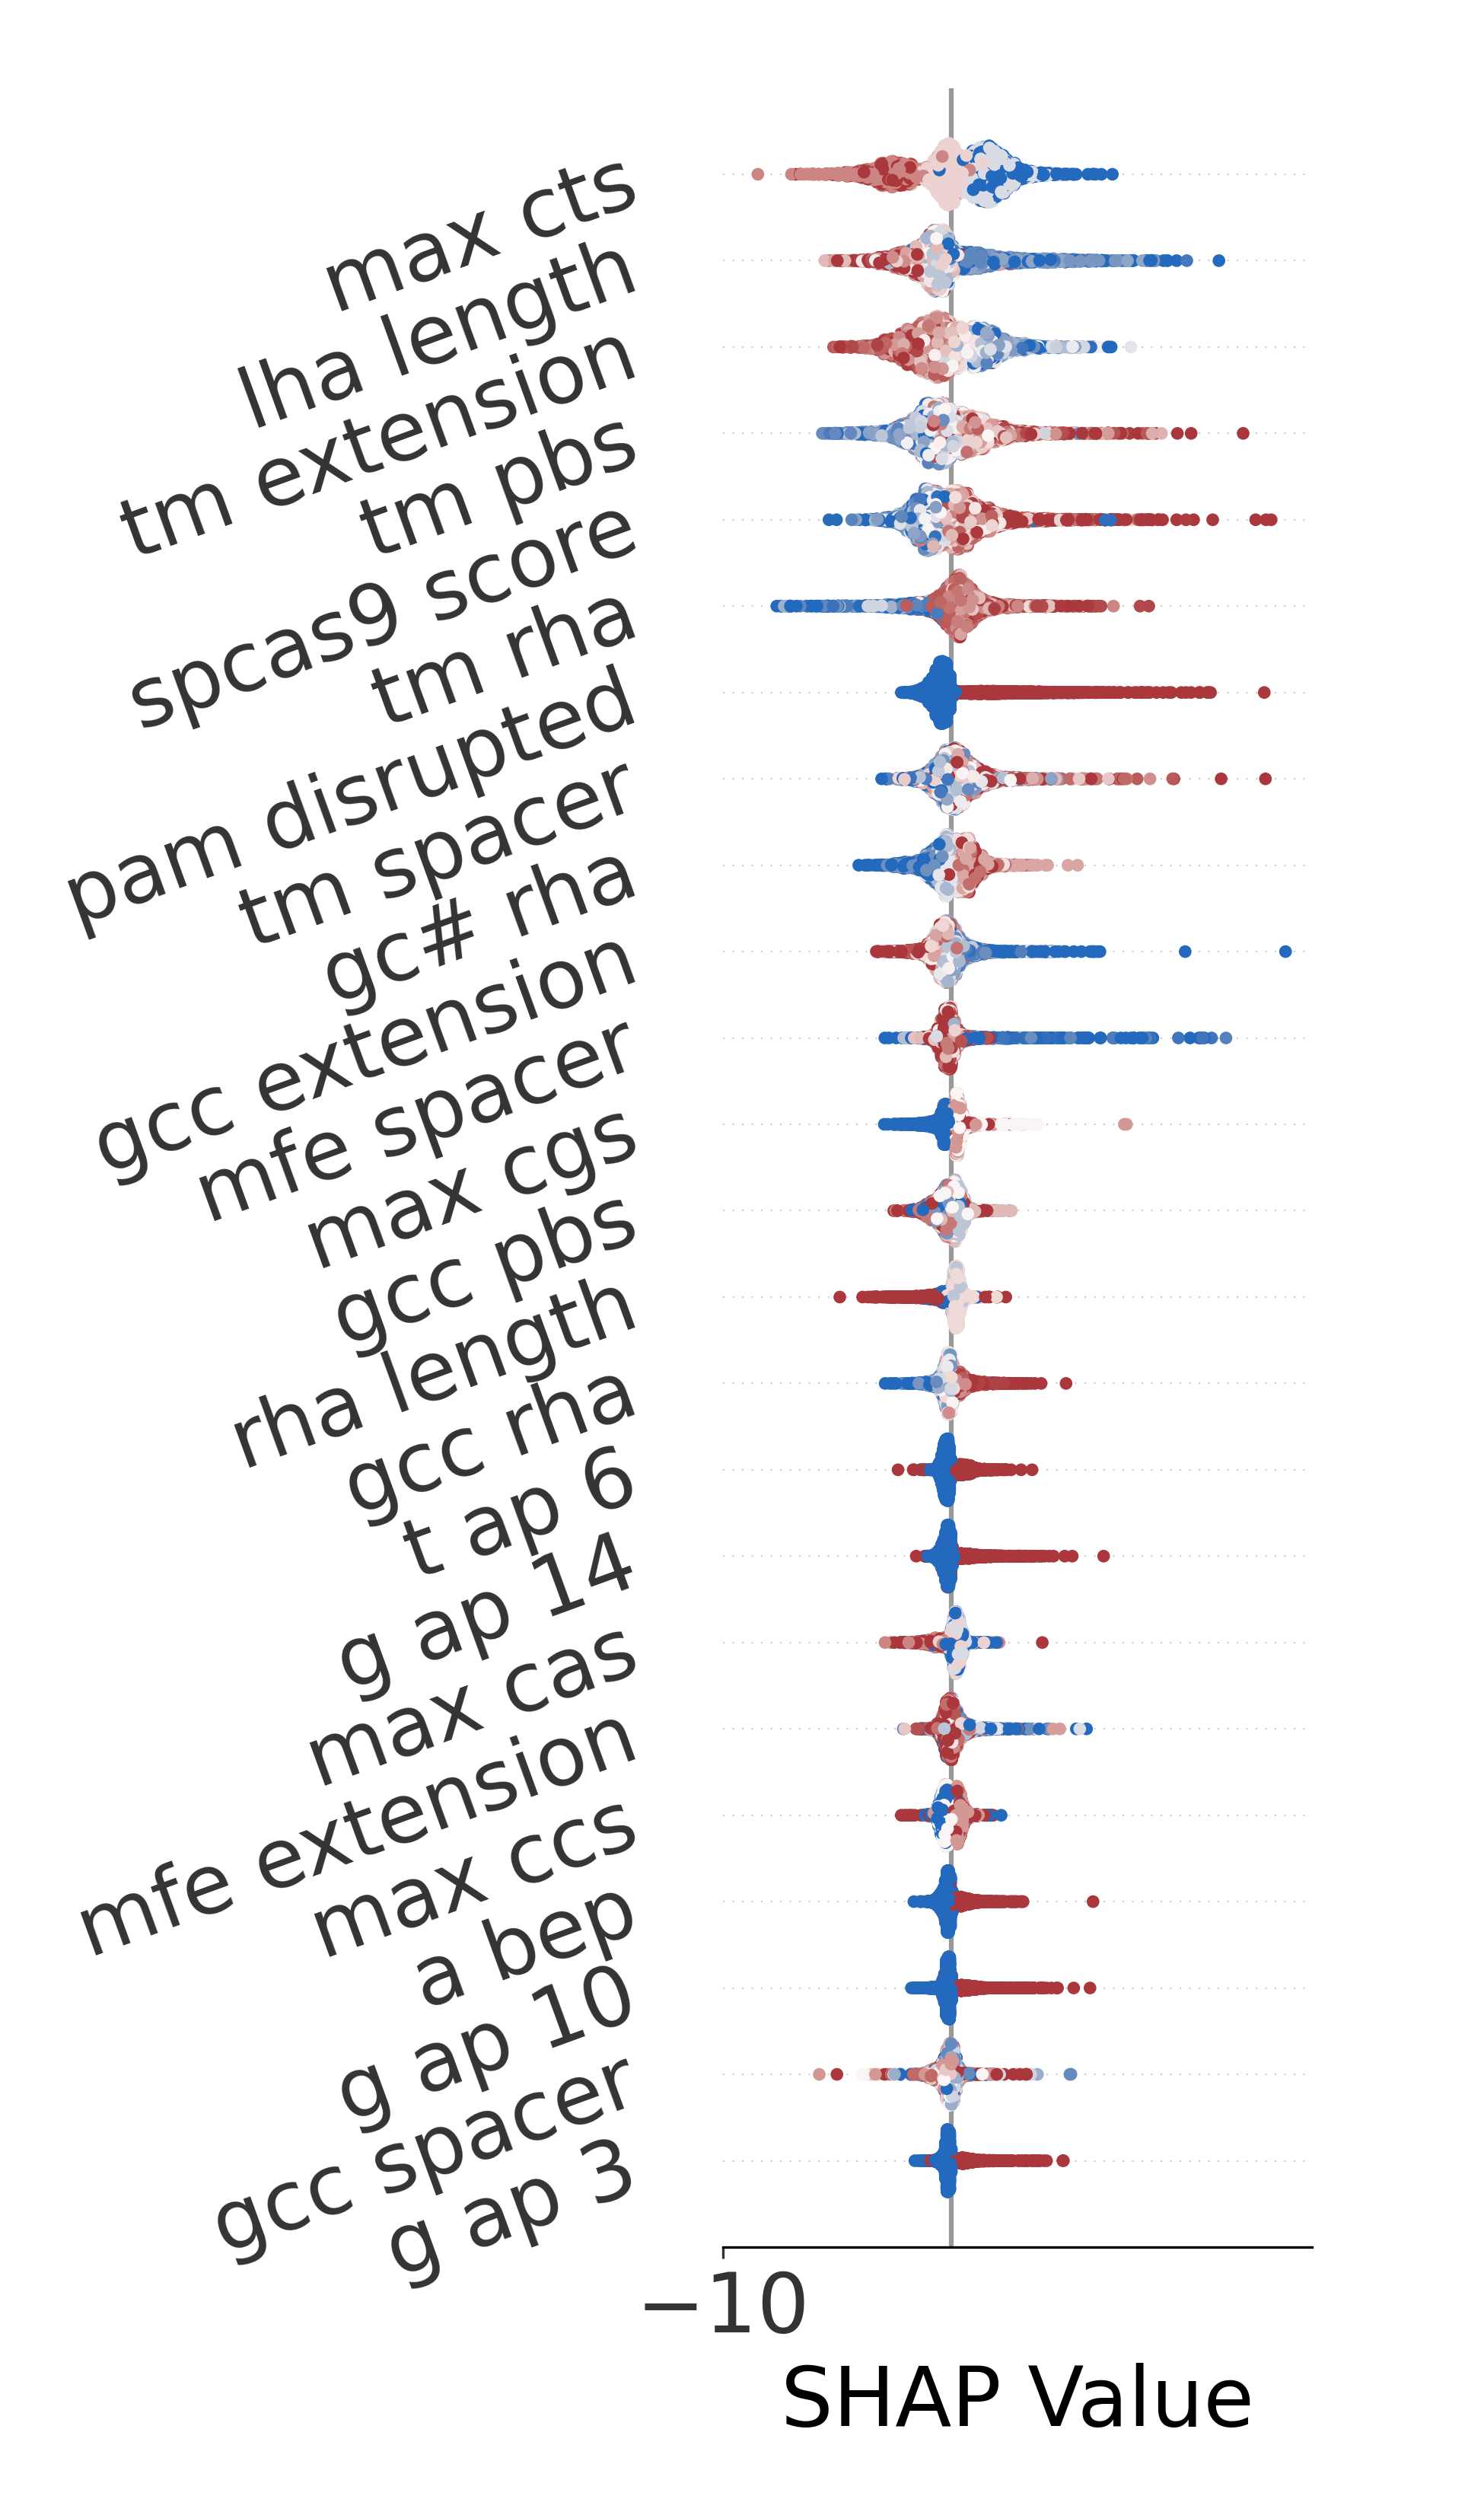
\includegraphics[width=0.33\textwidth]{shap_1bp-pd-k562-pe2-replace.png}
        \label{fig:shap-1bp-k562-pe2-replace}
    }%
    \subfigure[Insertion]{
        \centering
        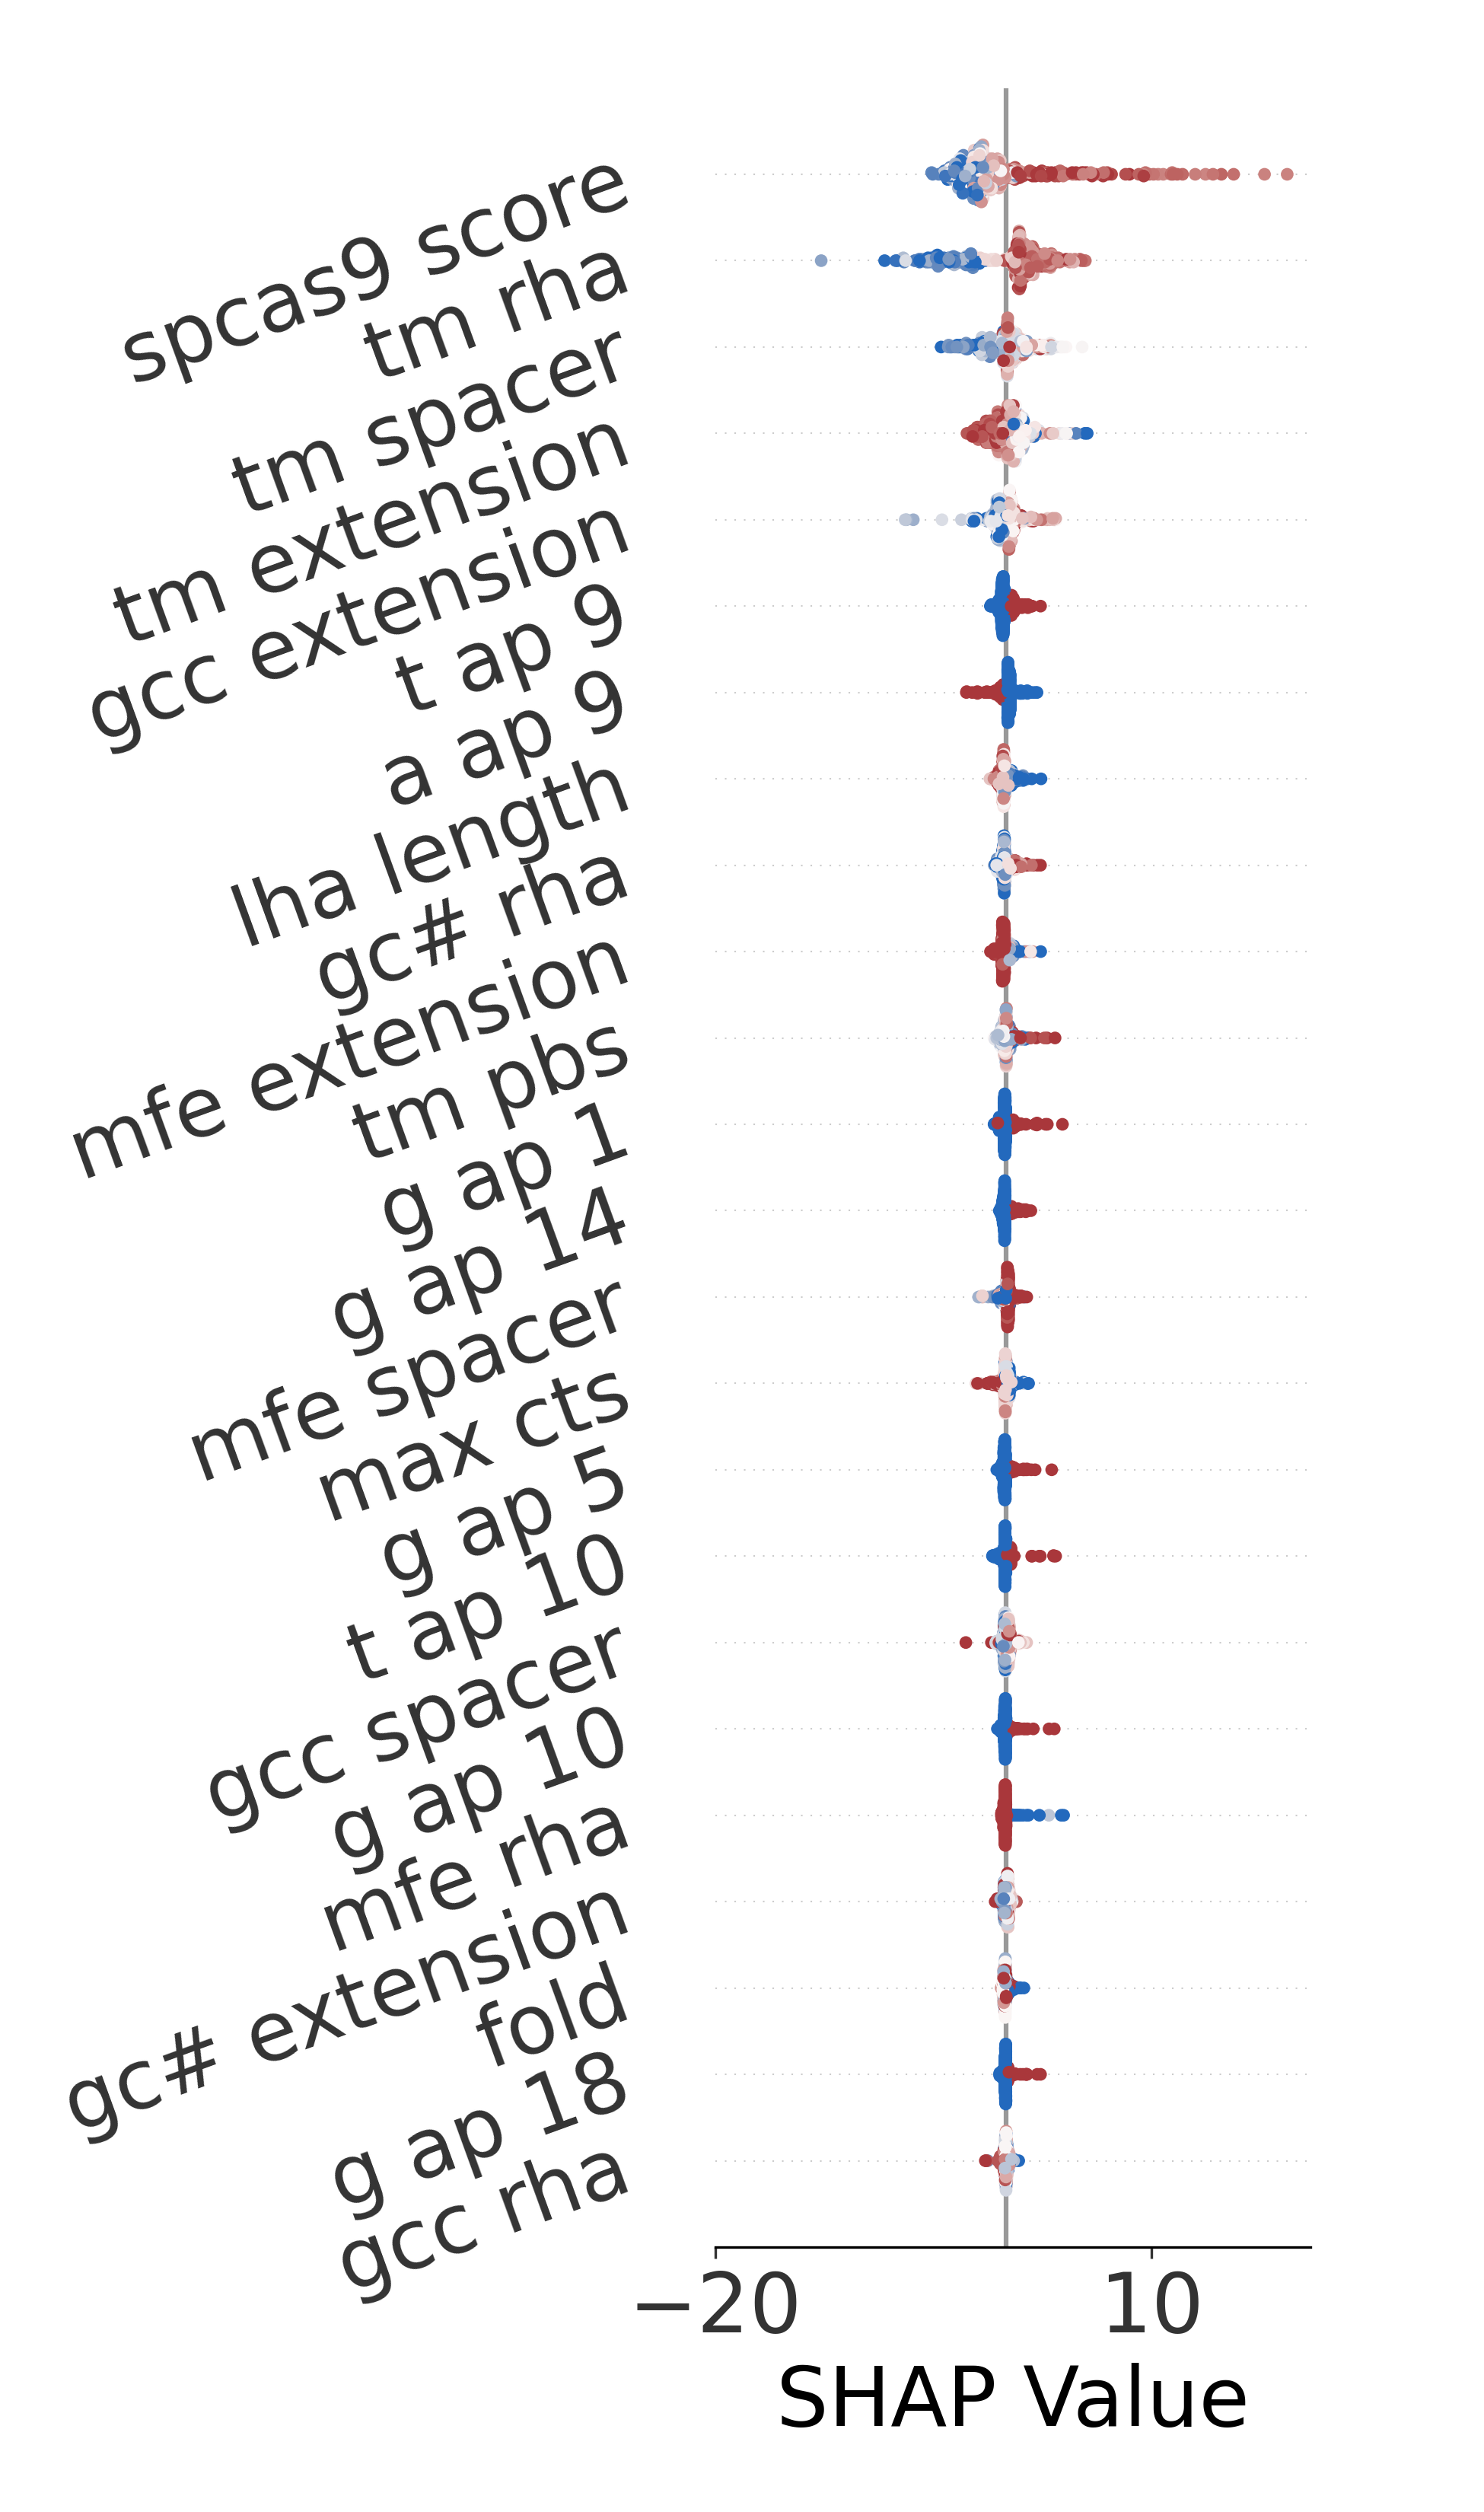
\includegraphics[width=0.33\textwidth]{shap_1bp-pd-k562-pe2-insert.png}
        \label{fig:shap-1bp-k562-pe2-insert}
    }%
    \subfigure[Deletion]{
        \centering
        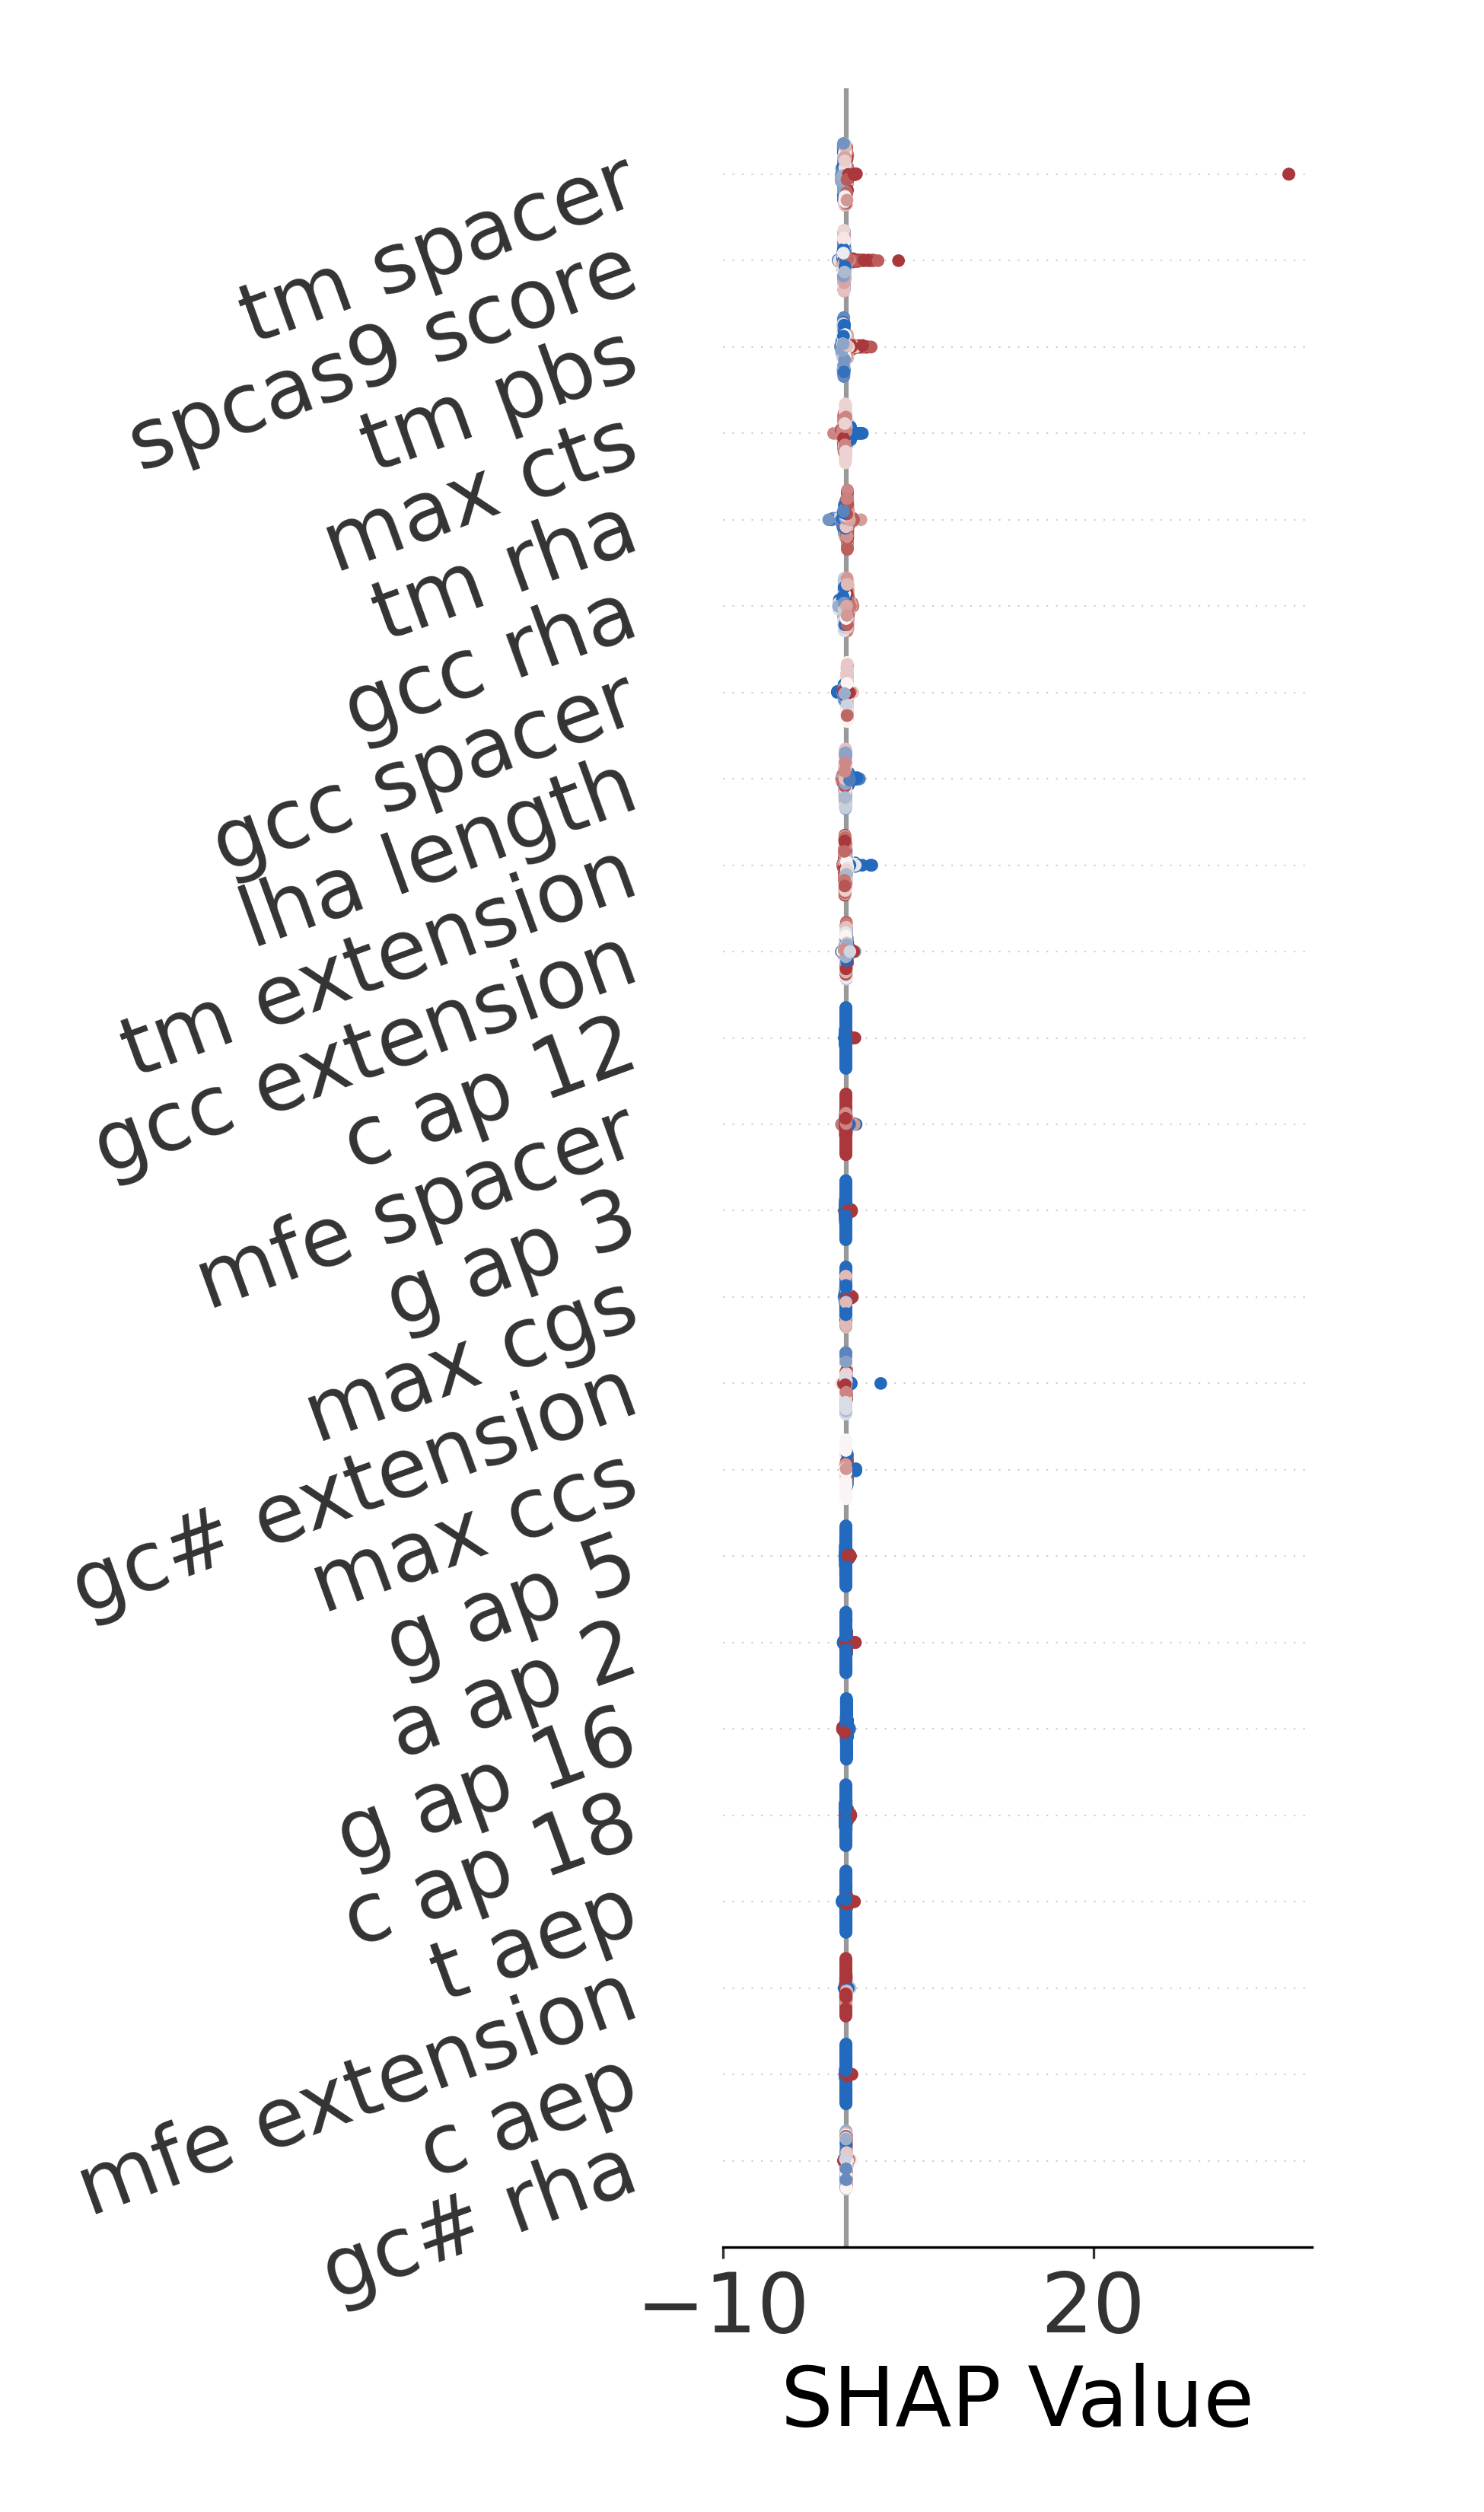
\includegraphics[width=0.33\textwidth]{shap_1bp-pd-k562-pe2-delete.png}
        \label{fig:shap-1bp-k562-pe2-delete}
    }
    \caption[SHAP Analysis of 1bp Edits on PRIDICT K562 PE2 Dataset]{SHAP Analysis of 1bp Edits on the PRIDICT K562 PE2 dataset.}
    \label{fig:shap-1bp-k562-pe2}
\end{figure}

\begin{figure}[!htb]
    \centering
    \subfigure[Substitution]{
        \centering
        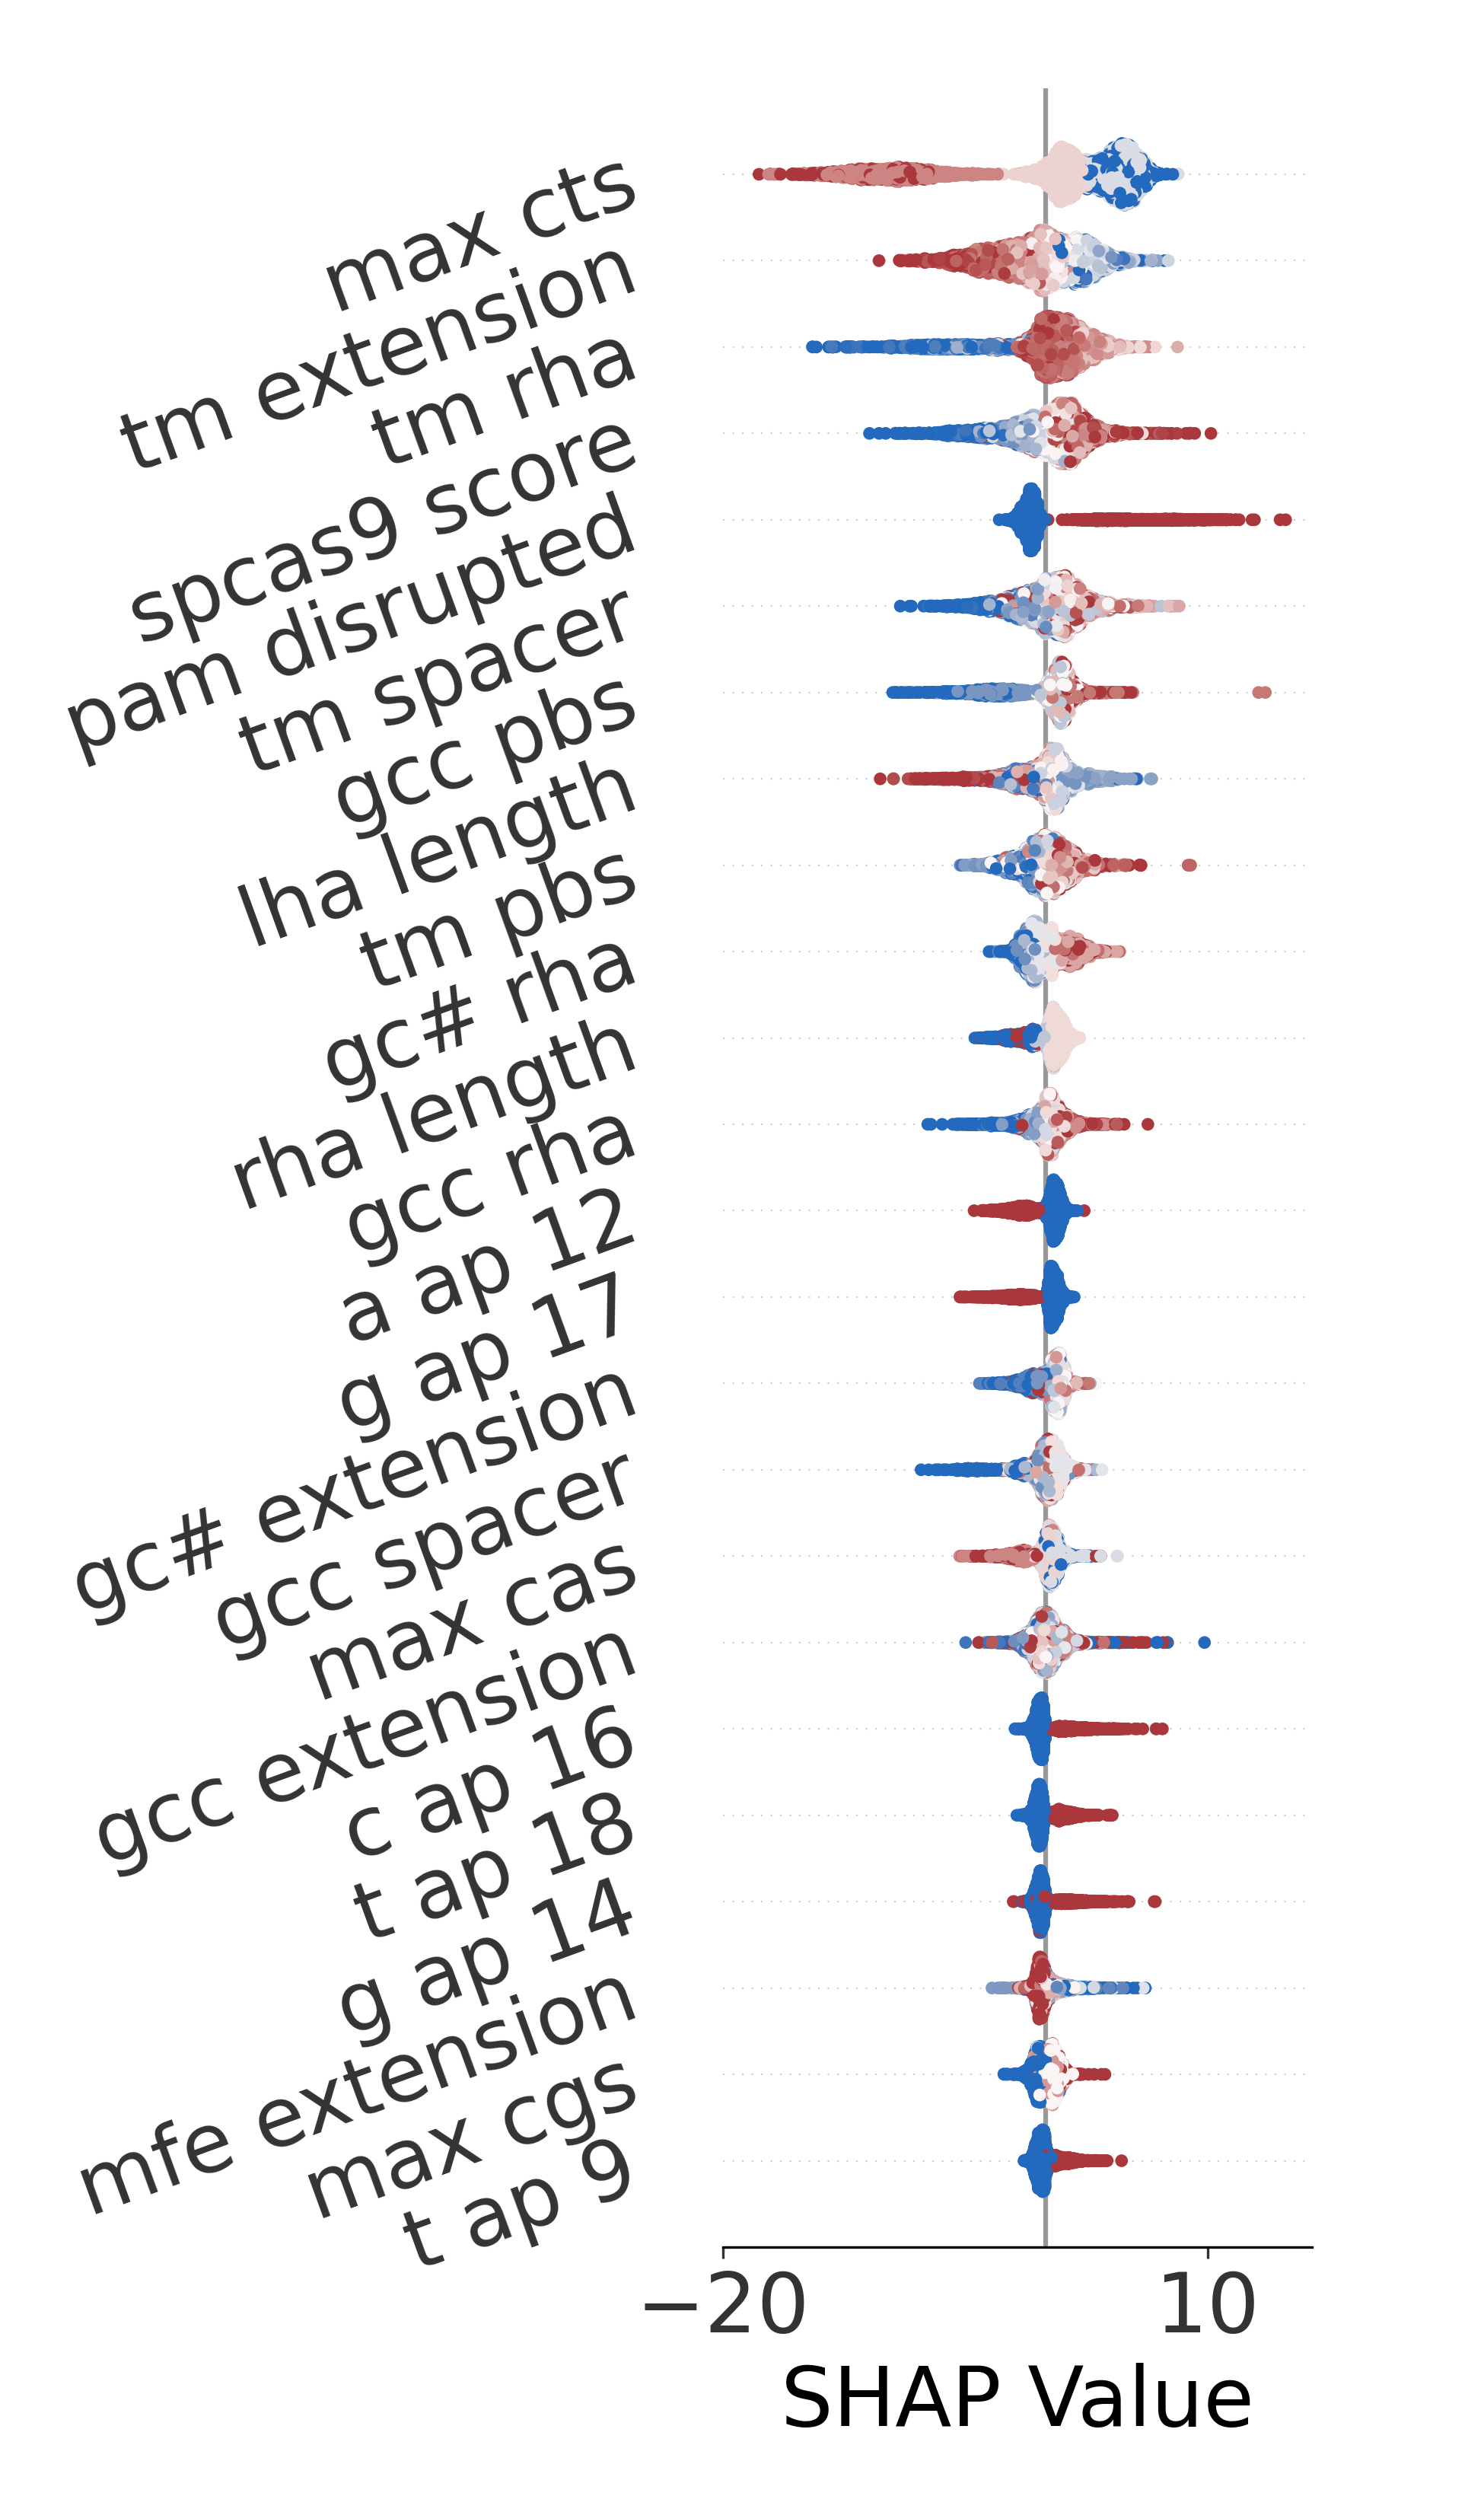
\includegraphics[width=0.33\textwidth]{shap_1bp-pd-k562mlh1dn-pe2-replace.png}
        \label{fig:shap-1bp-k562mlh1dn-pe2-replace}
    }%
    \subfigure[Insertion]{
        \centering
        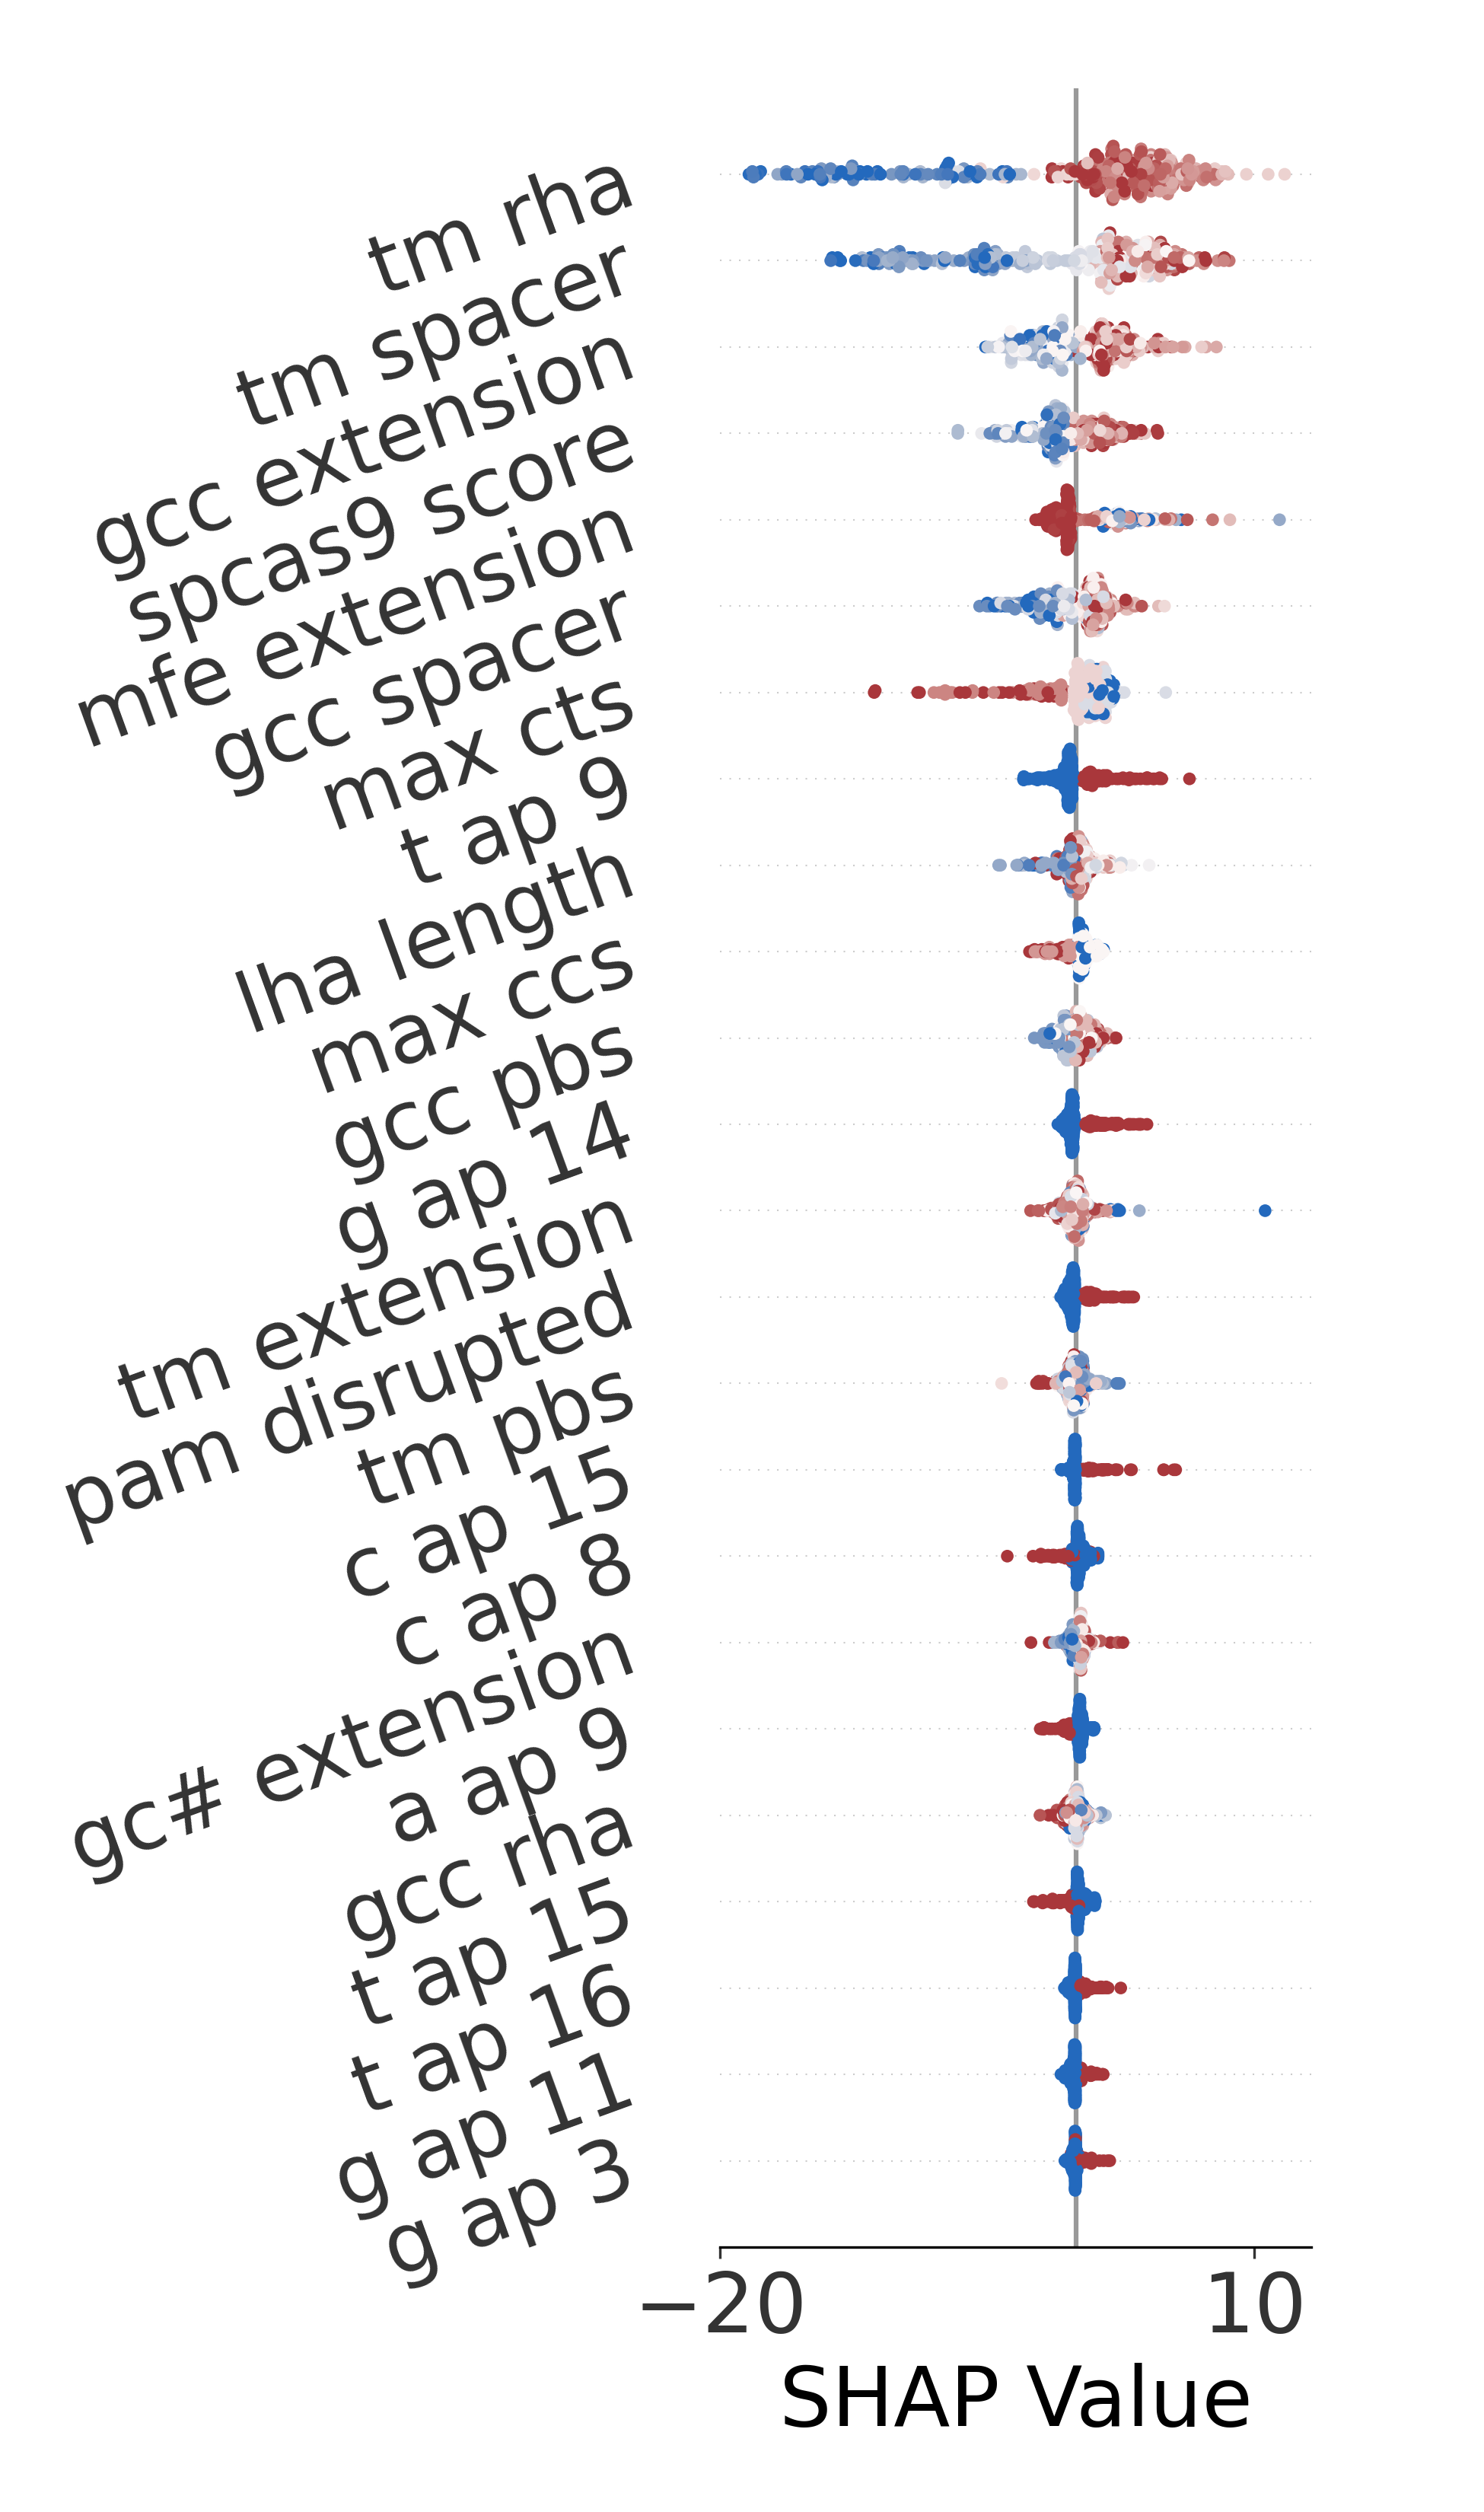
\includegraphics[width=0.33\textwidth]{shap_1bp-pd-k562mlh1dn-pe2-insert.png}
        \label{fig:shap-1bp-k562mlh1dn-pe2-insert}
    }%
    \subfigure[Deletion]{
        \centering
        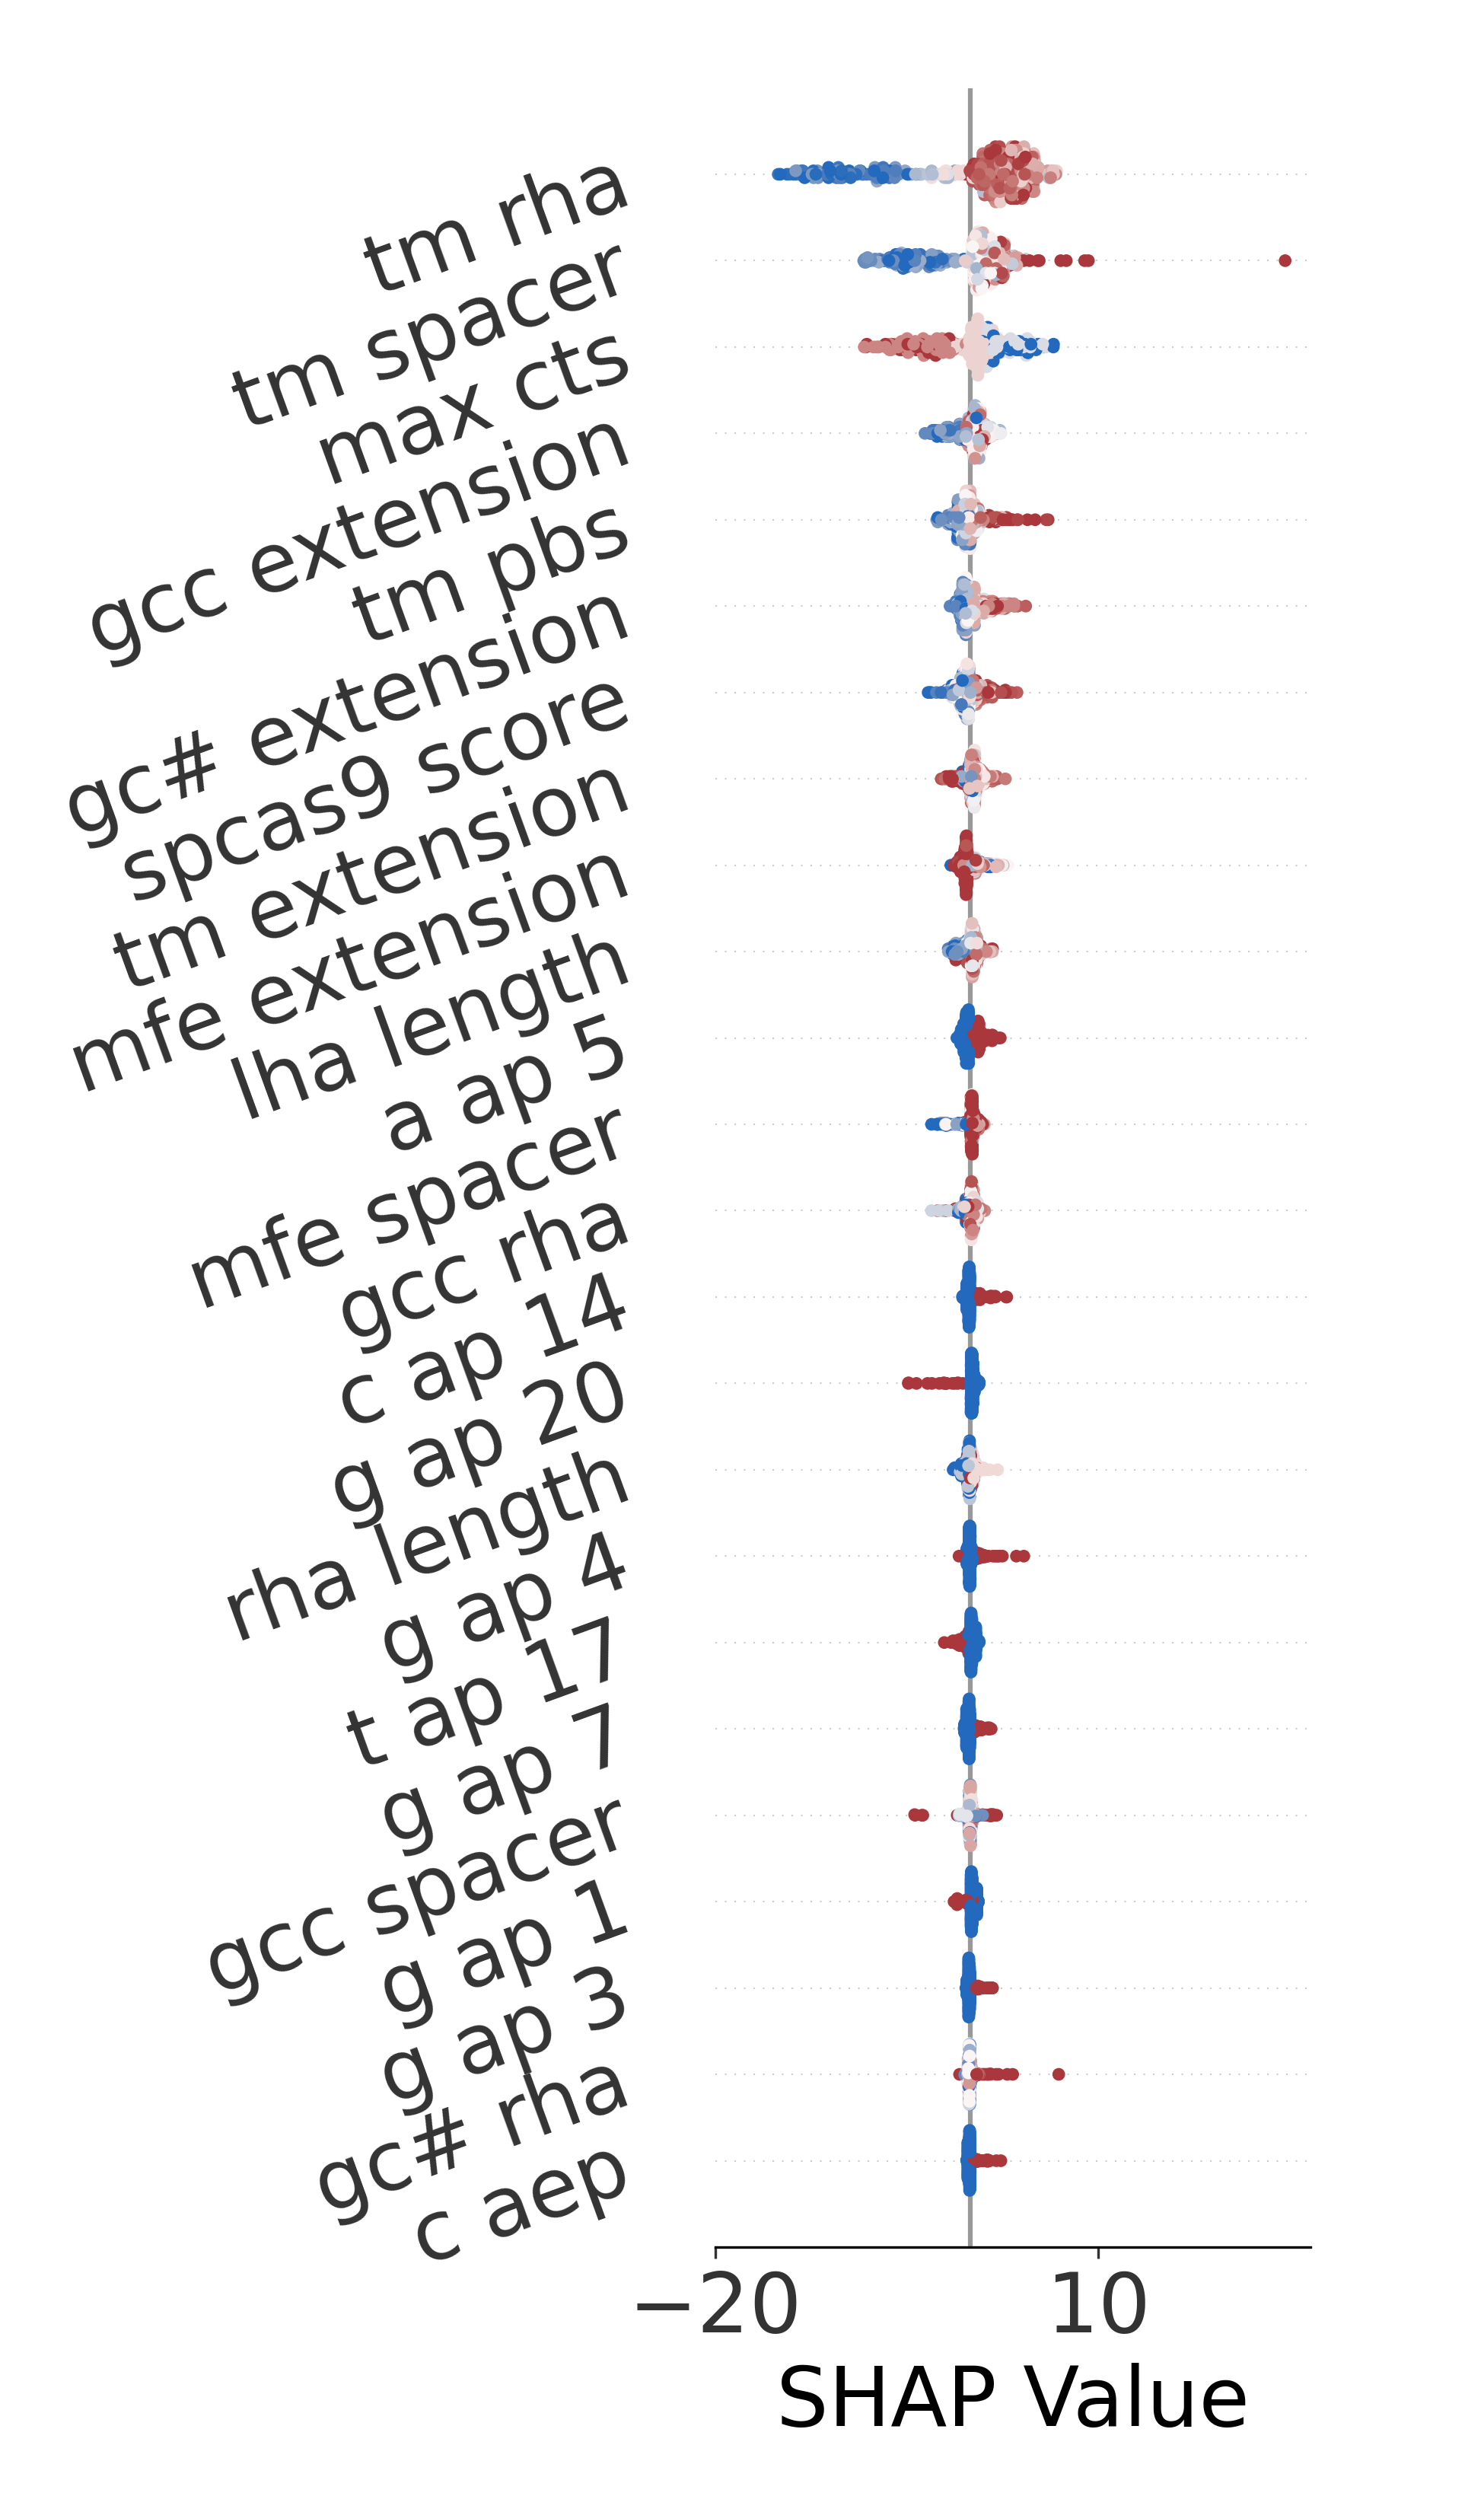
\includegraphics[width=0.33\textwidth]{shap_1bp-pd-k562mlh1dn-pe2-delete.png}
        \label{fig:shap-1bp-k562mlh1dn-pe2-delete}
    }
    \caption[SHAP Analysis of 1bp Edits on PRIDICT K562 MLH1 DN PE2 Dataset]{SHAP Analysis of 1bp Edits on the PRIDICT K562 MLH1 DN PE2 dataset.}
    \label{fig:shap-1bp-k562mlh1dn-pe2}
\end{figure}

\begin{figure}[!htb]
    \centering
    \subfigure[Substitution]{
        \centering
        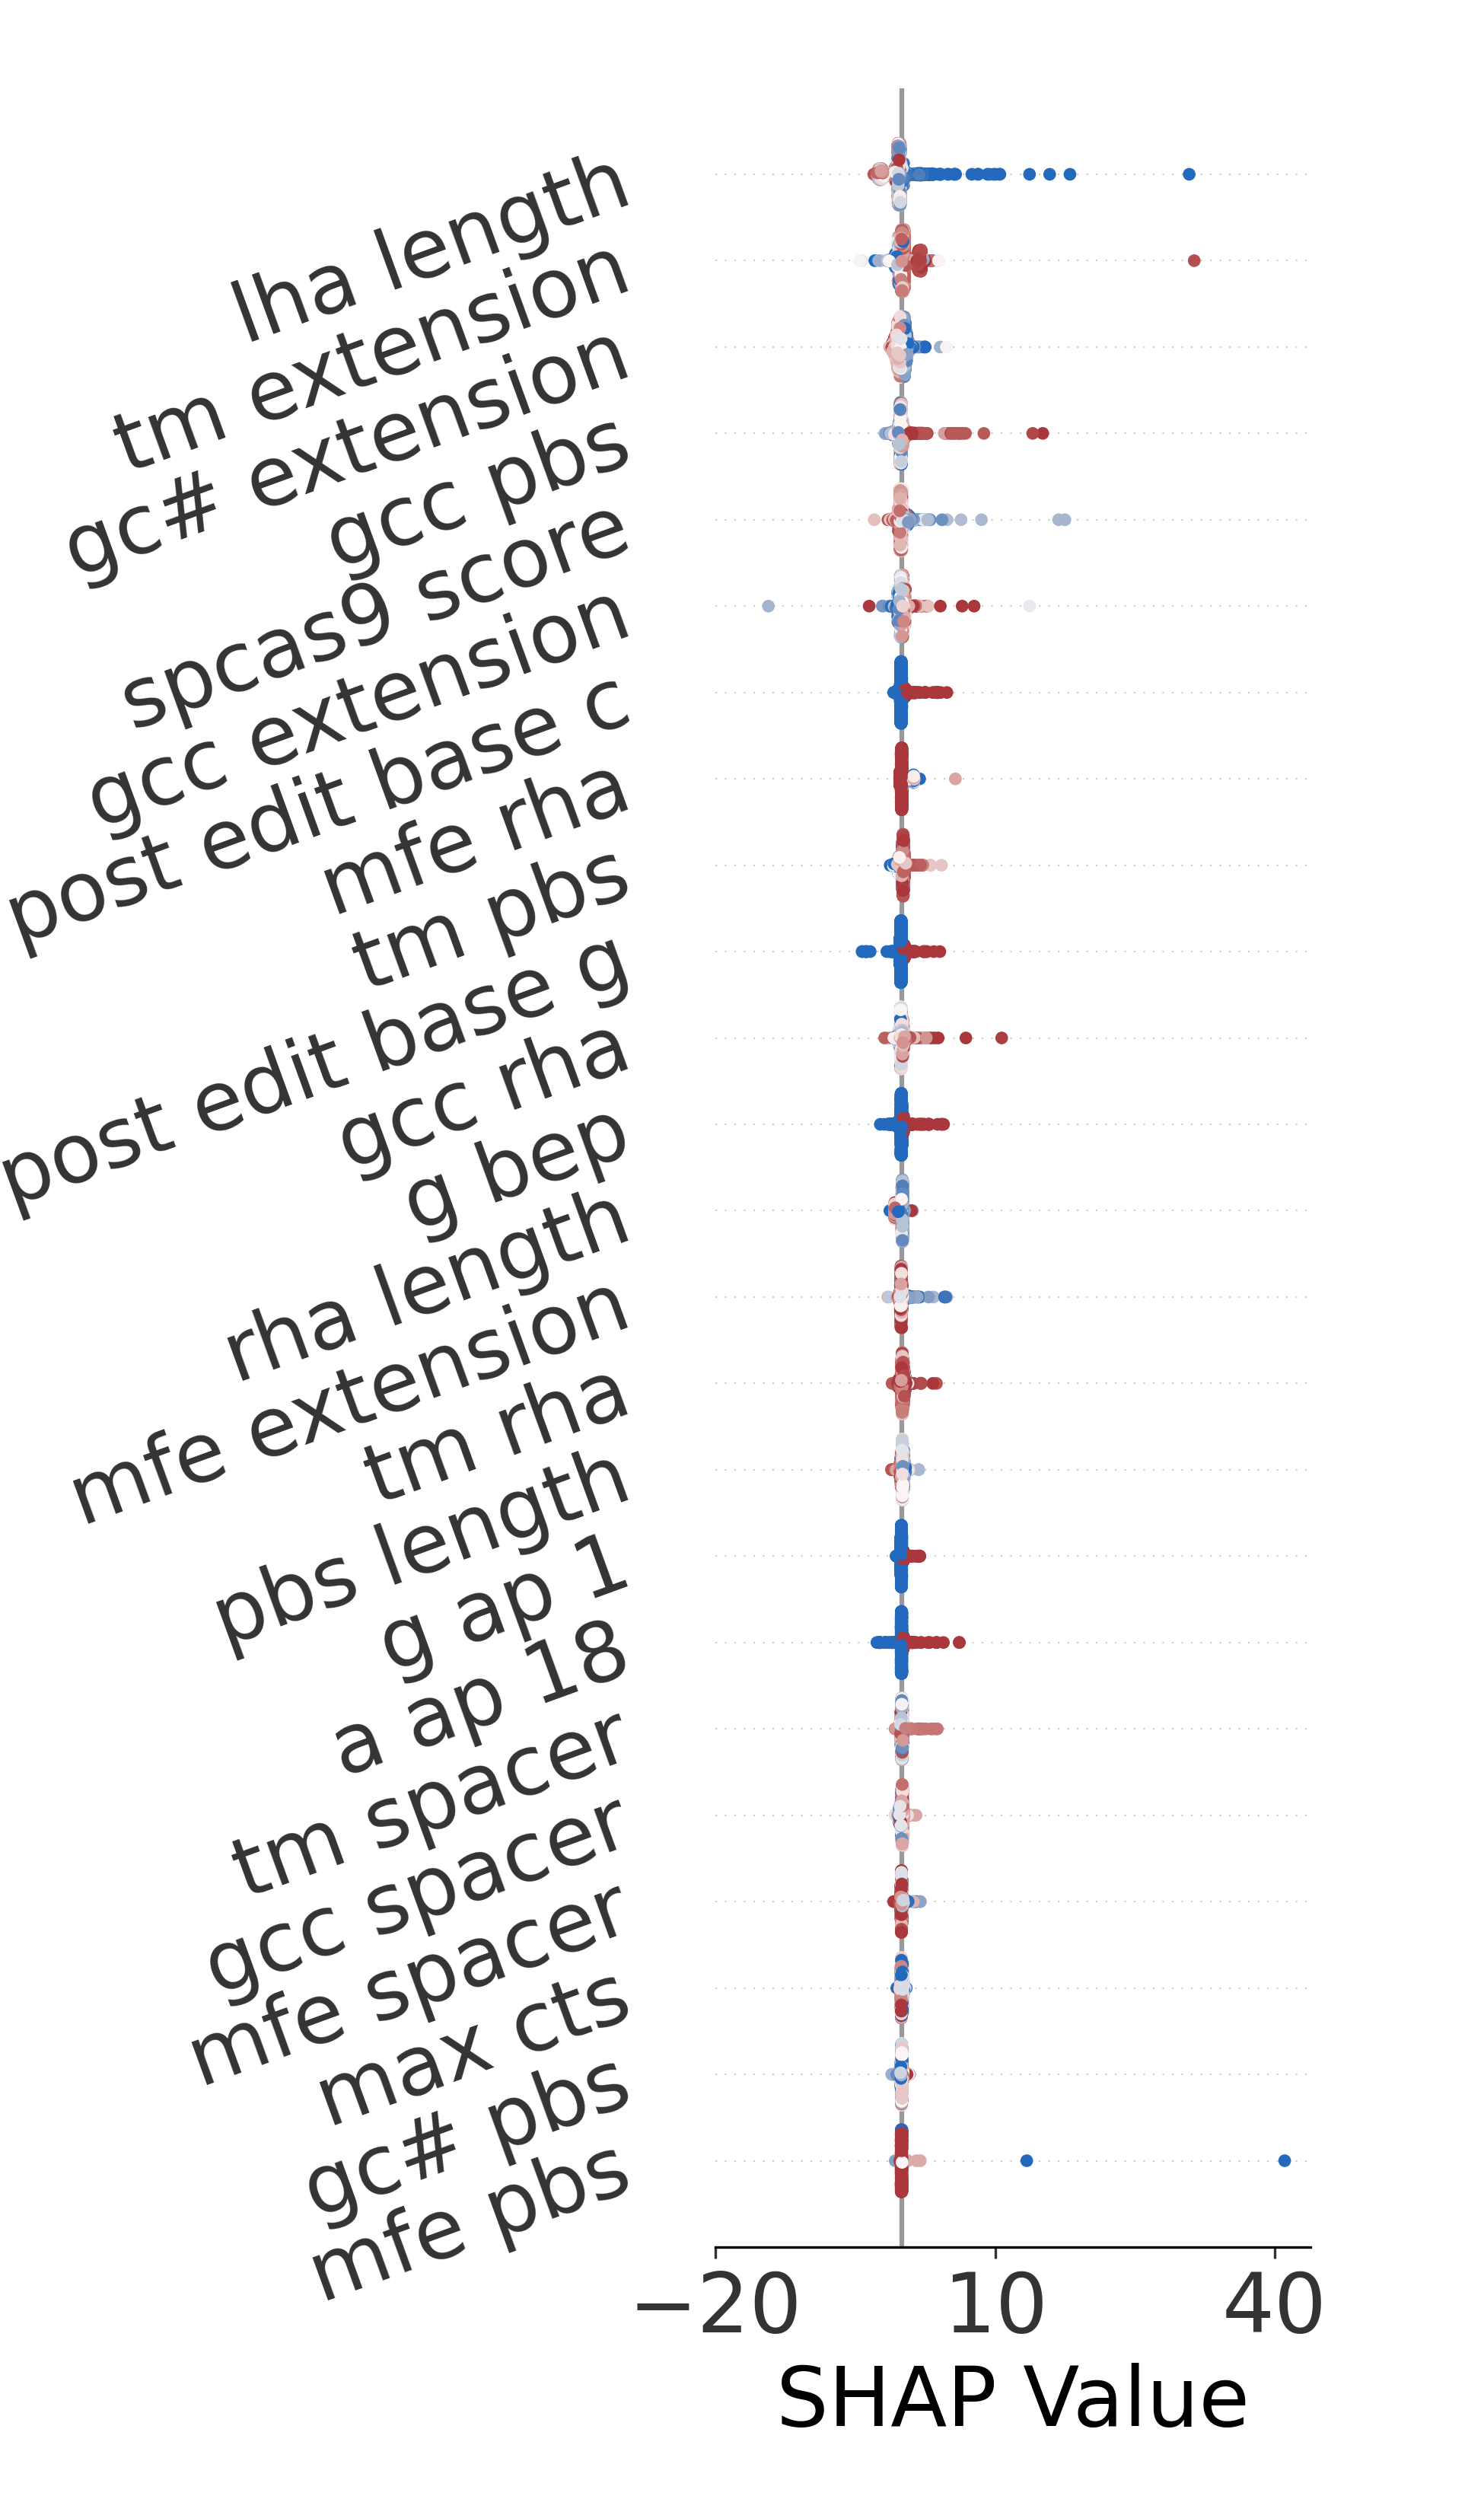
\includegraphics[width=0.33\textwidth]{shap_1bp-dp_small-a549-pe2max-replace.png}
        \label{fig:shap-1bp-a549-pe2max-replace}
    }%
    \subfigure[Insertion]{
        \centering
        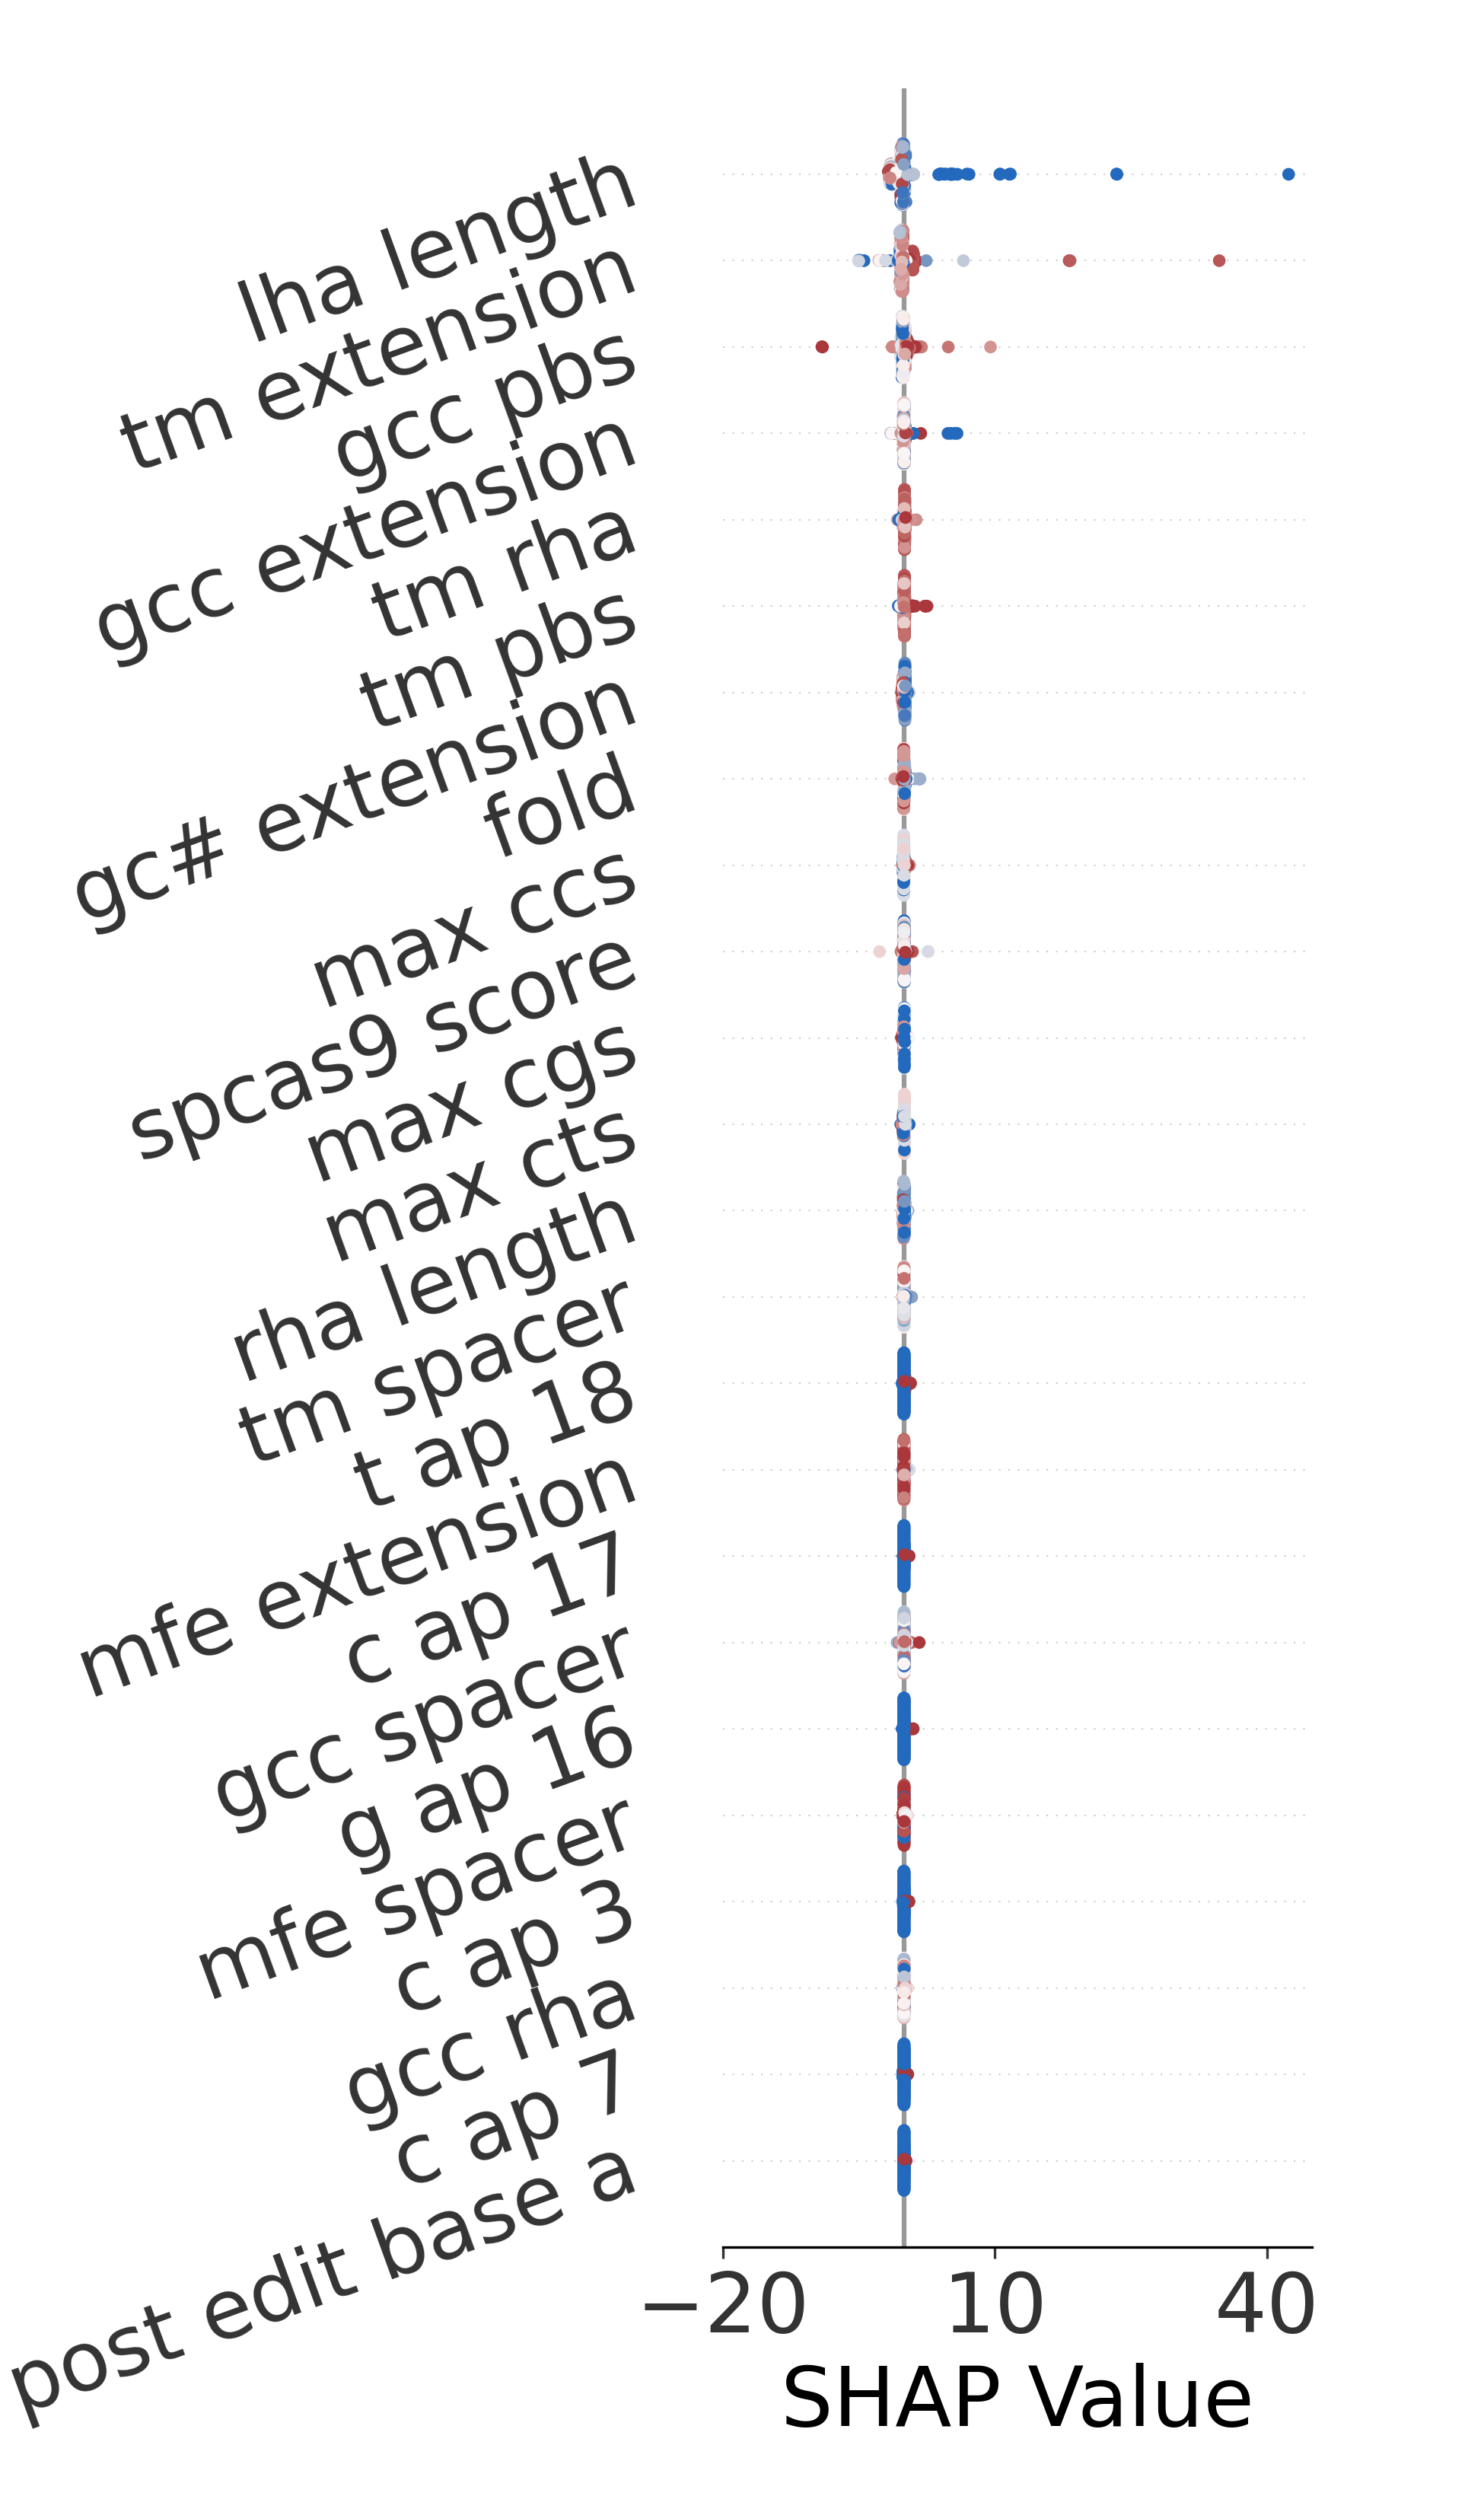
\includegraphics[width=0.33\textwidth]{shap_1bp-dp_small-a549-pe2max-insert.png}
        \label{fig:shap-1bp-a549-pe2max-insert}
    }%
    \subfigure[Deletion]{
        \centering
        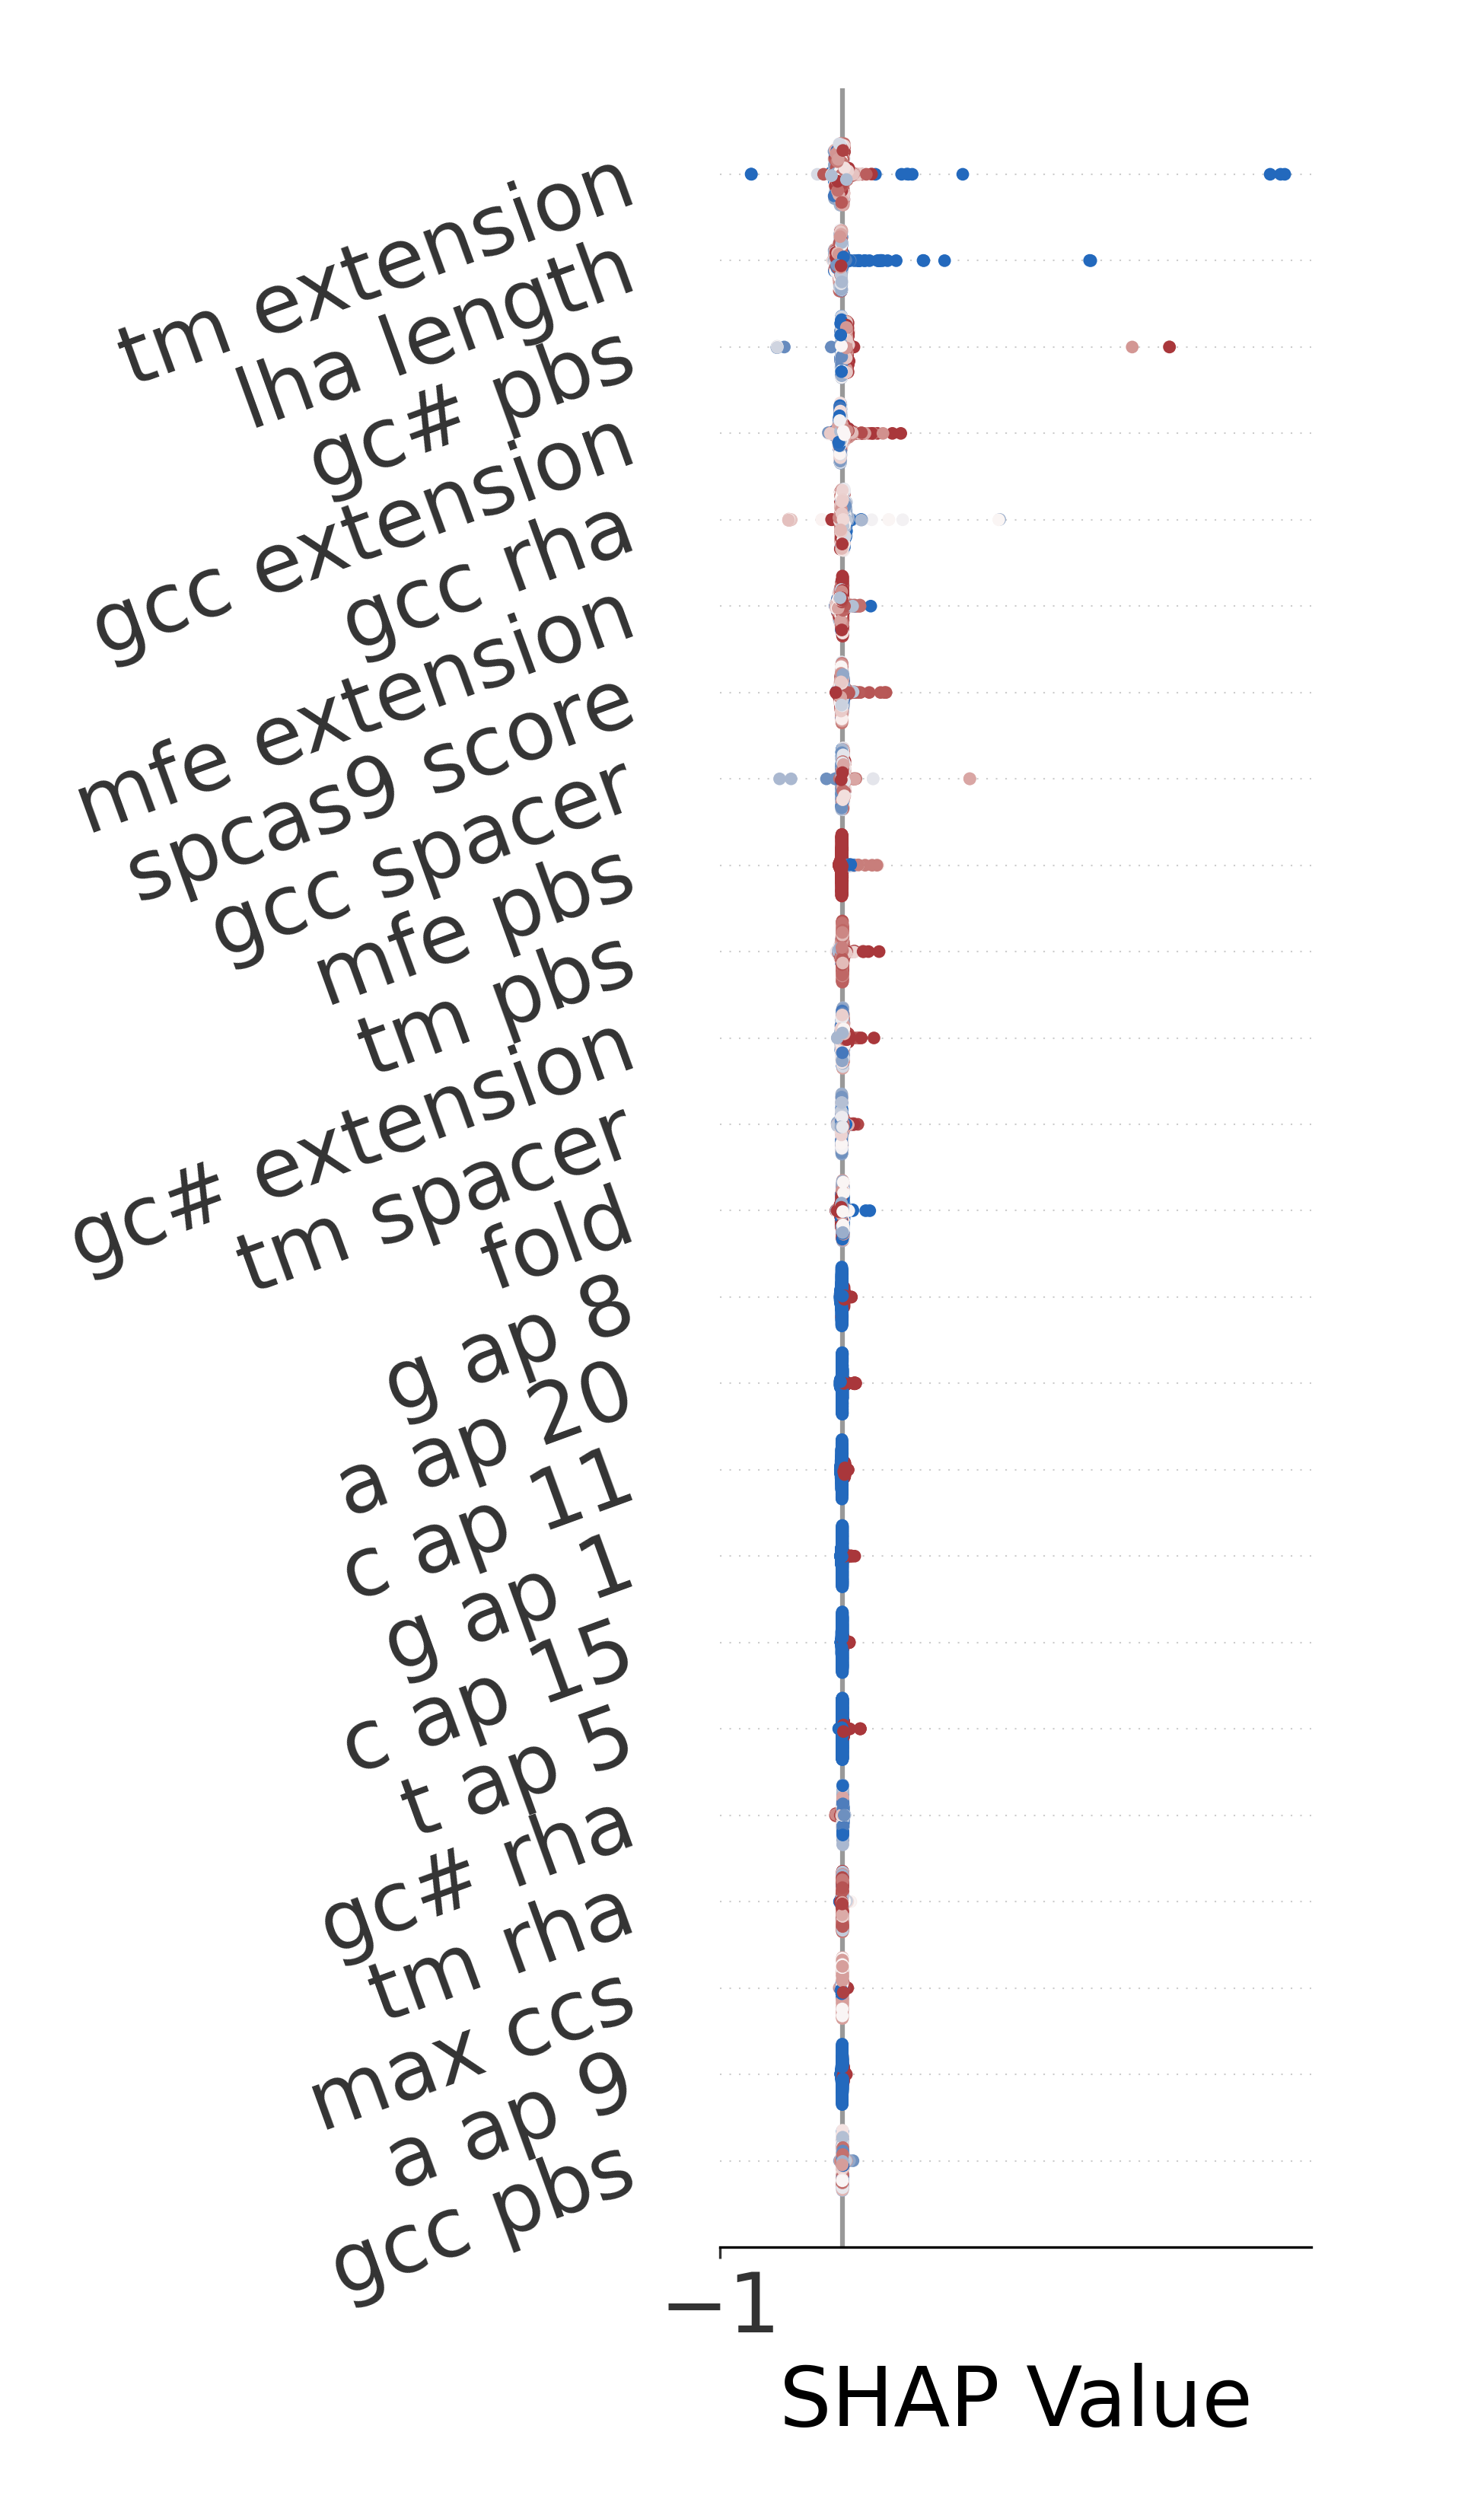
\includegraphics[width=0.33\textwidth]{shap_1bp-dp_small-a549-pe2max-delete.png}
        \label{fig:shap-1bp-a549-pe2max-delete}
    }
    \caption[SHAP Analysis of 1bp Edits on PRIDICT A549 PE2MAX Dataset]{SHAP Analysis of 1bp Edits on the PRIDICT A549 PE2MAX dataset.}
    \label{fig:shap-1bp-a549-pe2max}
\end{figure}

